\documentclass[12pt]%[english]
{article}

\usepackage{graphicx,subfigure}
\usepackage{microtype}
\usepackage[nonumberlist, acronym, toc, section]{glossaries}
\usepackage{cite} 


%% additional packages and commands
\usepackage{amsmath}
\usepackage{amssymb}

% to format pseudo code
\usepackage{algorithm}% http://ctan.org/pkg/algorithms
\usepackage{algpseudocode}% http://ctan.org/pkg/algorithmicx

% make numbers in circles: https://tex.stackexchange.com/questions/7032/good-way-to-make-textcircled-numbers
\usepackage{tikz}
\usetikzlibrary{shapes.misc}

\newcommand*\circled[1]{\tikz[baseline=(char.base)]{
            \node[shape=circle,draw,inner sep=1pt] (char) {#1};}}
% alternative to that: \raisebox{.5pt}{\textcircled{\raisebox{-.9pt} {8}}}

\usepackage{pdfpages} % to embed pdfs
\usepackage{multicol}

% for code snippets
\usepackage{minted}
\usepackage{xcolor}
\definecolor{code-bg}{rgb}{0.95,0.95,0.95}

\usepackage{wrapfig}

\usepackage{url}

\newglossary[slg]{symbolslist}{syi}{syg}{Symbols}

\makeglossaries

%commands for symbols
\newglossaryentry{symb:Pi}{
name=$\pi$,
description={You know it.},
sort=symbolpi, type=symbolslist
}
\newglossaryentry{symb:Phi}{
name=$\varphi$,
description={At vero eos et accusam et justo duo dolores et ea rebum..},
sort=symbolphi, type=symbolslist
}
\newglossaryentry{symb:Lambda}{
name=$\lambda$,
description={Lorem ipsum dolor sit amet, consetetur sadipscing elitr, sed diam nonumy.},
sort=symbollambda, type=symbolslist
}

%commands for abbreviations
\newacronym{MS}{MS}{Microsoft}
\newacronym{CD}{CD}{Compact Disc}
\newacronym{sklearn}{sklearn}{Scikit-Learn}

\newacronym{DI}{DI}{Dunn Index}
\newacronym{CH}{CH}{Calinski-Harabasz Index}
\newacronym{DB}{DB}{Davies-Bouldin Index}
\newacronym{SI}{SI}{Silhouette Score}
\newacronym{GS}{GS}{Gap Statistic}
\newacronym{VRC}{VRC}{Variance Ratio Criterion}
\newacronym{t-SNE}{t-SNE}{t-distributed Stochastic Neighbor Embedding}


% ...

%abbreviations and glossary combined
\newacronym{AD}{AD}{Active Directory\protect\glsadd{glos:AD}}
%\newacronym{sklearn}{sklearn}{Scikit-Learn\protect\glsadd{glos:sklearn}}
 
% ... 
 
%glossary commands

\newglossaryentry{glos:AD}{
name=Active Directory,
description={At vero eos et accusam et justo duo dolores et ea rebum. Stet clita kasd gubergren, no sea takimata sanctus est Lorem ipsum dolor sit amet}
}

\newglossaryentry{glos:F}{name=File, description={An arbitrary file}}

% ...

\begin{document}

\begin{titlepage}
\begin{center}

{\Huge {
Term Paper Data Science 1}
}
\\[2ex]

\textbf{
\Large 
Docent: Prof. Dr. Lena Wiese \\ 
Semester: Summer Term 2021\\  
}




\includegraphics[scale=0.4]{images/logo.jpg} \\ 
\large{\textbf{Institute of Computer Science \\ Goethe-Universit\"at Frankfurt a. M.}}



\begin{normalsize}
\begin{tabular}{ll}
& \\
Author: & $\textsc{M. A.}$ \\
& $\langle$your Student ID$\rangle$\\
& $\langle$your.email@ddre.ss$\rangle$ \\
& $\langle$branch of study (Bachelor/Master, semester count)$\rangle$ \\
& $\textsc{L. B.}$ \\
& $\langle$your Student ID$\rangle$\\
& $\langle$your.email@ddre.ss$\rangle$ \\
& $\langle$branch of study (Bachelor/Master, semester count)$\rangle$ \\
& $\textsc{B. L.}$ \\
& $\langle$your Student ID$\rangle$\\
& $\langle$your.email@ddre.ss$\rangle$ \\
& $\langle$branch of study (Bachelor/Master, semester count)$\rangle$ \\
& $\textsc{J. M.}$ \\
& $\langle$your Student ID$\rangle$\\
& $\langle$your.email@ddre.ss$\rangle$ \\
& $\langle$branch of study (Bachelor/Master, semester count)$\rangle$ \\
Date: & \today \\		
\end{tabular}
\end{normalsize}

\end{center}

\vspace*{\fill}

\large
\noindent{}Chosen Project Topic: % \\
\begin{itemize}
\item T3 Clustering
\end{itemize}
\noindent{}Github Repository: % \\
\begin{itemize}
\item \url{https://github.com/BenLucht/DS1_term_paper}
\end{itemize}
\end{titlepage}

\newpage\thispagestyle{empty}~ %empty page
\newpage 

\begin{abstract}
Not done yet.
\end{abstract}

\newpage

\tableofcontents

\newpage

\section{Problem Description}
\label{sec:problem_description}
Clustering is a long-known method in the field of Data Science and Machine Learning. It describes the process of grouping elements of a given dataset into a finite number of distinct segments such that the elements of one segment are as similar as possible to one another while maximizing the dissimilarity between different segments. The resulting segments are called clusters. Finding clusters is of interest to gain information on patterns or structures characterizing a given dataset \cite{madhulatha2012overview}.
Each of the given data points is interpreted as a multidimensional feature vector and clusters are found by calculating vector similarities. Similarity or dissimilarity is measured using different kinds of metrics which are chosen according to the underlying data space \cite{rokach2005Clustering}.

As no a priori knowledge about the given dataset is assumed, distinguishing it from classification contexts, clustering is an unsupervised learning method. There exist several different clustering techniques which differ in their embedded assumptions on the cluster shapes or the requirement of various parameters such as the number of clusters or the bandwidth.

There is a wide variety of applications for clustering methods in research and professional contexts ranging from social network analysis to image compression and even oil well operation.

In this report, K-Means Clustering, Affinity Propagation Clustering, Mean Shift Clustering and Spectral Clustering are investigated.

Each of these clustering algorithms is applied on each of the chosen datasets and clustering performance is evaluated using cluster validation indexes. In the end, results generated applying the different algorithms are compared to each other. 

% \begin{itemize}
% \item What general problem is addressed?
% \item What is the general methodology that is used?
% \end{itemize}
% 
% Some Latex-specific hints:
% 
% 
% \begin{itemize}
% \item You can use abbreviations, like \gls{AD}, \gls{MS} or \gls{CD}.
% \item There are also symbols like for example \gls{symb:Pi}, \gls{symb:Phi} % and \gls{symb:Lambda}.
% \item Last but not least, use glossary entries like \gls{glos:AD} and % \gls{glos:F}.
% \item Do not forget to cite related work, like \cite{okman2011security} or % \cite{borthakur2011apache}.
% \end{itemize}

\section{Description of Specific Methods and Algorithms}
\label{sec:method_descriptions}
% \begin{itemize}
% \item What benchmark data sets are used?
% \end{itemize}

\subsection{Boston House Pricing Data}
\textit{written by L.B.}\\

The Boston House Pricing data set was originally published in 1978 by Harrison and Rubinfeld \cite{hedonichousepricing}. In their study the authors used the data set to investigate how people's willingness to pay for clean air is correlated with different measurements of house data around the area of Boston.
In total, 506 samples are included within the data set, containing fourteen different attribute columns. Six of those attribute values originate from the U.S. Census Service, the remaining originate amongst others from the FBI, the Metropolitan Area Planning Commission, the Massachusetts Taxpayers Foundation, the Massachusetts Department of Education and the MIT Boston project. All data was sampled in 1970. The attributes of each data can be separated into different types, providing information on structure, neighborhood, accessibility or air pollution.

Structural attributes yield information on the state of the house with respect to year of construction or spaciousness. While the \textit{RM} variable holds the numeric value for the average number of rooms, the \textit{AGE} attribute describes the proportion of houses that were built before 1940. Both values are assumed to have a positive correlation with housing values since owning more rooms or owning houses with modern structures is perceived as increasing life quality. 

Neighborhood attributes hold details about the socioeconomic status of the environment. This includes the fraction of colored people in the whole population, as well as the \textit{LSTAT} attribute, which denotes the amount of people being of lower educational status. In addition to that, crime rate is included for neighborhoods of Boston area. The latter attribute is supposed to have a negative effect on housing values as crime rate influences people's level of danger. 
Another neighborhood attribute stands for the sum of square feet available for residential zoning where constructing buildings like factories is prohibited. Next, the \textit{INDUS} attribute comprises the proportion of industry which comes along with noise, traffic and dirt and is therefore negatively correlated with housing values. Moreover, property tax rate as well as the ratio between pupils and teachers are included. The last socioeconomic attribute classifies whether the respective city area adjoins Charles River.

Accessibility attributes characterize infrastructure measured by closeness to employment centers and to radial highways. 

In order to estimate air quality, the concentration of Nitrogen Oxid in parts per hundred million is measured. 

The last attribute is the dependent variable which describes the median value of houses that are occupied by private owners. 

While the index of highway accessibility is an integer value and the closeness to Charles River is described using a binary variable encoded as 0 and 1, the remaining attributes are float numbers. The data set does not contain any empty columns, thus no elimination or preprocessing of the available data is necessary.\newline
Table \ref{tab:housing_table} provides some general statistics on the given data set. For each of the columns except the measurement of closeness to Charles River, mean, minimum and maximum value as well as the standard deviation are given. In addition to that, lower (0.25) and upper (0.75) quartiles and the 50\%-quantiles are listed for each of the thirteen features. Quantiles yield information on how the data points are distributed within the high-dimensional feature space. It can be observed that for most of the features, data points lie relatively close together, proposing the data set to consist of dense regions. 

\begin{table}[H]
    \centering
    \begin{tabular}{c|c|c|c|c|c|c|c}
          \hline
         Column & Mean & Min & Max & Std & 25\% & 50\% & 75\%  \\
        \hline
         CRIM & 3.614 & 0.006 & 88.976 & 8.593 & 0.082 & 0.257 & 3.677\\
         ZN & 11.364 & 0.000 & 100.000 & 23.299 & 0.000 & 0.000 & 12.5\\
         INDUS & 11.137 & 0.460 & 27.740 & 6.854 & 5.190 & 9.960 & 18.100\\
         NOX & 0.555 & 0.385 & 0.871 & 0.116 & 0.449 & 0.538 & 0.624\\
         RM & 6.285 & 3.561 & 8.780 & 0.702 & 5.886 & 6.209 & 6.624\\
         AGE & 68.575 & 2.900 & 100.000 & 28.121 & 45.025 & 77.500 & 94.075\\
         DIS & 3.795 & 1.130 & 12.127 & 2.104 & 2.100 & 3.207 & 5.188\\
         RAD & 9.549 & 1.000 & 24.000 & 8.699 & 4.000 & 5.000 & 24.000\\
         TAX & 408.237 & 187.000 & 711.000 & 168.371 & 279.000 & 330.000 & 666.000\\
         PTRATIO & 18.456 & 12.600 & 22.000 & 2.163 & 17.400 & 19.050 & 20.200\\
         B & 356.674 & 0.320 & 396.9 & 91.205 & 375.378 & 391.44 & 396.225\\
         LSTAT & 12.653 & 1.730 & 37.970 & 7.134 & 6.950 & 11.360 & 16.955\\
         MEDV & 22.533 & 5.000 & 50.000 & 9.188 & 17.025 & 21.200 & 25.000\\
    \end{tabular}
    \caption{General Statistics on Boston House Pricing Data Set}
    \label{tab:housing_table}
\end{table}
\subsection{Mall Customer Segmentation}
\textit{by J. M.}\\

The Data Set Mall Customer Segmentation Data includes basic customer data. It contains a unique Id for each customer, gender, age, the annual income, and the spending Score. In this Score you can have a value between 1 and 100. The distribution of gender of the customer is 56\% female and 44 \% male. In the preprocessing every entry of the gender column gets a number 0 or 1 depending on the gender is male or female. I do this because than every entry of this dataset contains only numbers. The Age of the Customers is between 18 und 70. The Annual Income of the customers is between 15 and 127. 
\subsection{Seeds Data}

This data set has been used in the work of \cite{charytanowicz2010complete}. The data comprises information on different features of wheat kernels. There are seven species with a total of about 20 varieties of which three can be found in the data: Kama, Rosa and Canadian wheat. There is a total of 210 data points, evenly split between the varieties. The kernels for which data was collected were selected randomly. They were then examined through X-ray imaging. A software called \textit{GRAINS} for this specific application \cite{strumillo1999computer} was used to extract the features for each observation:
\begin{multicols}{2}
\begin{itemize}
\item area $A$
\item perimeter $P$
\item compactness $C = 4 \pi A/P^{2}$
\item length (along groove)
\item width
\item asymmetry coefficient
\item length of kernel groove
\item label
\end{itemize}
\end{multicols}

\begin{figure}[h]
\caption{Seeds pairplot WIP}
%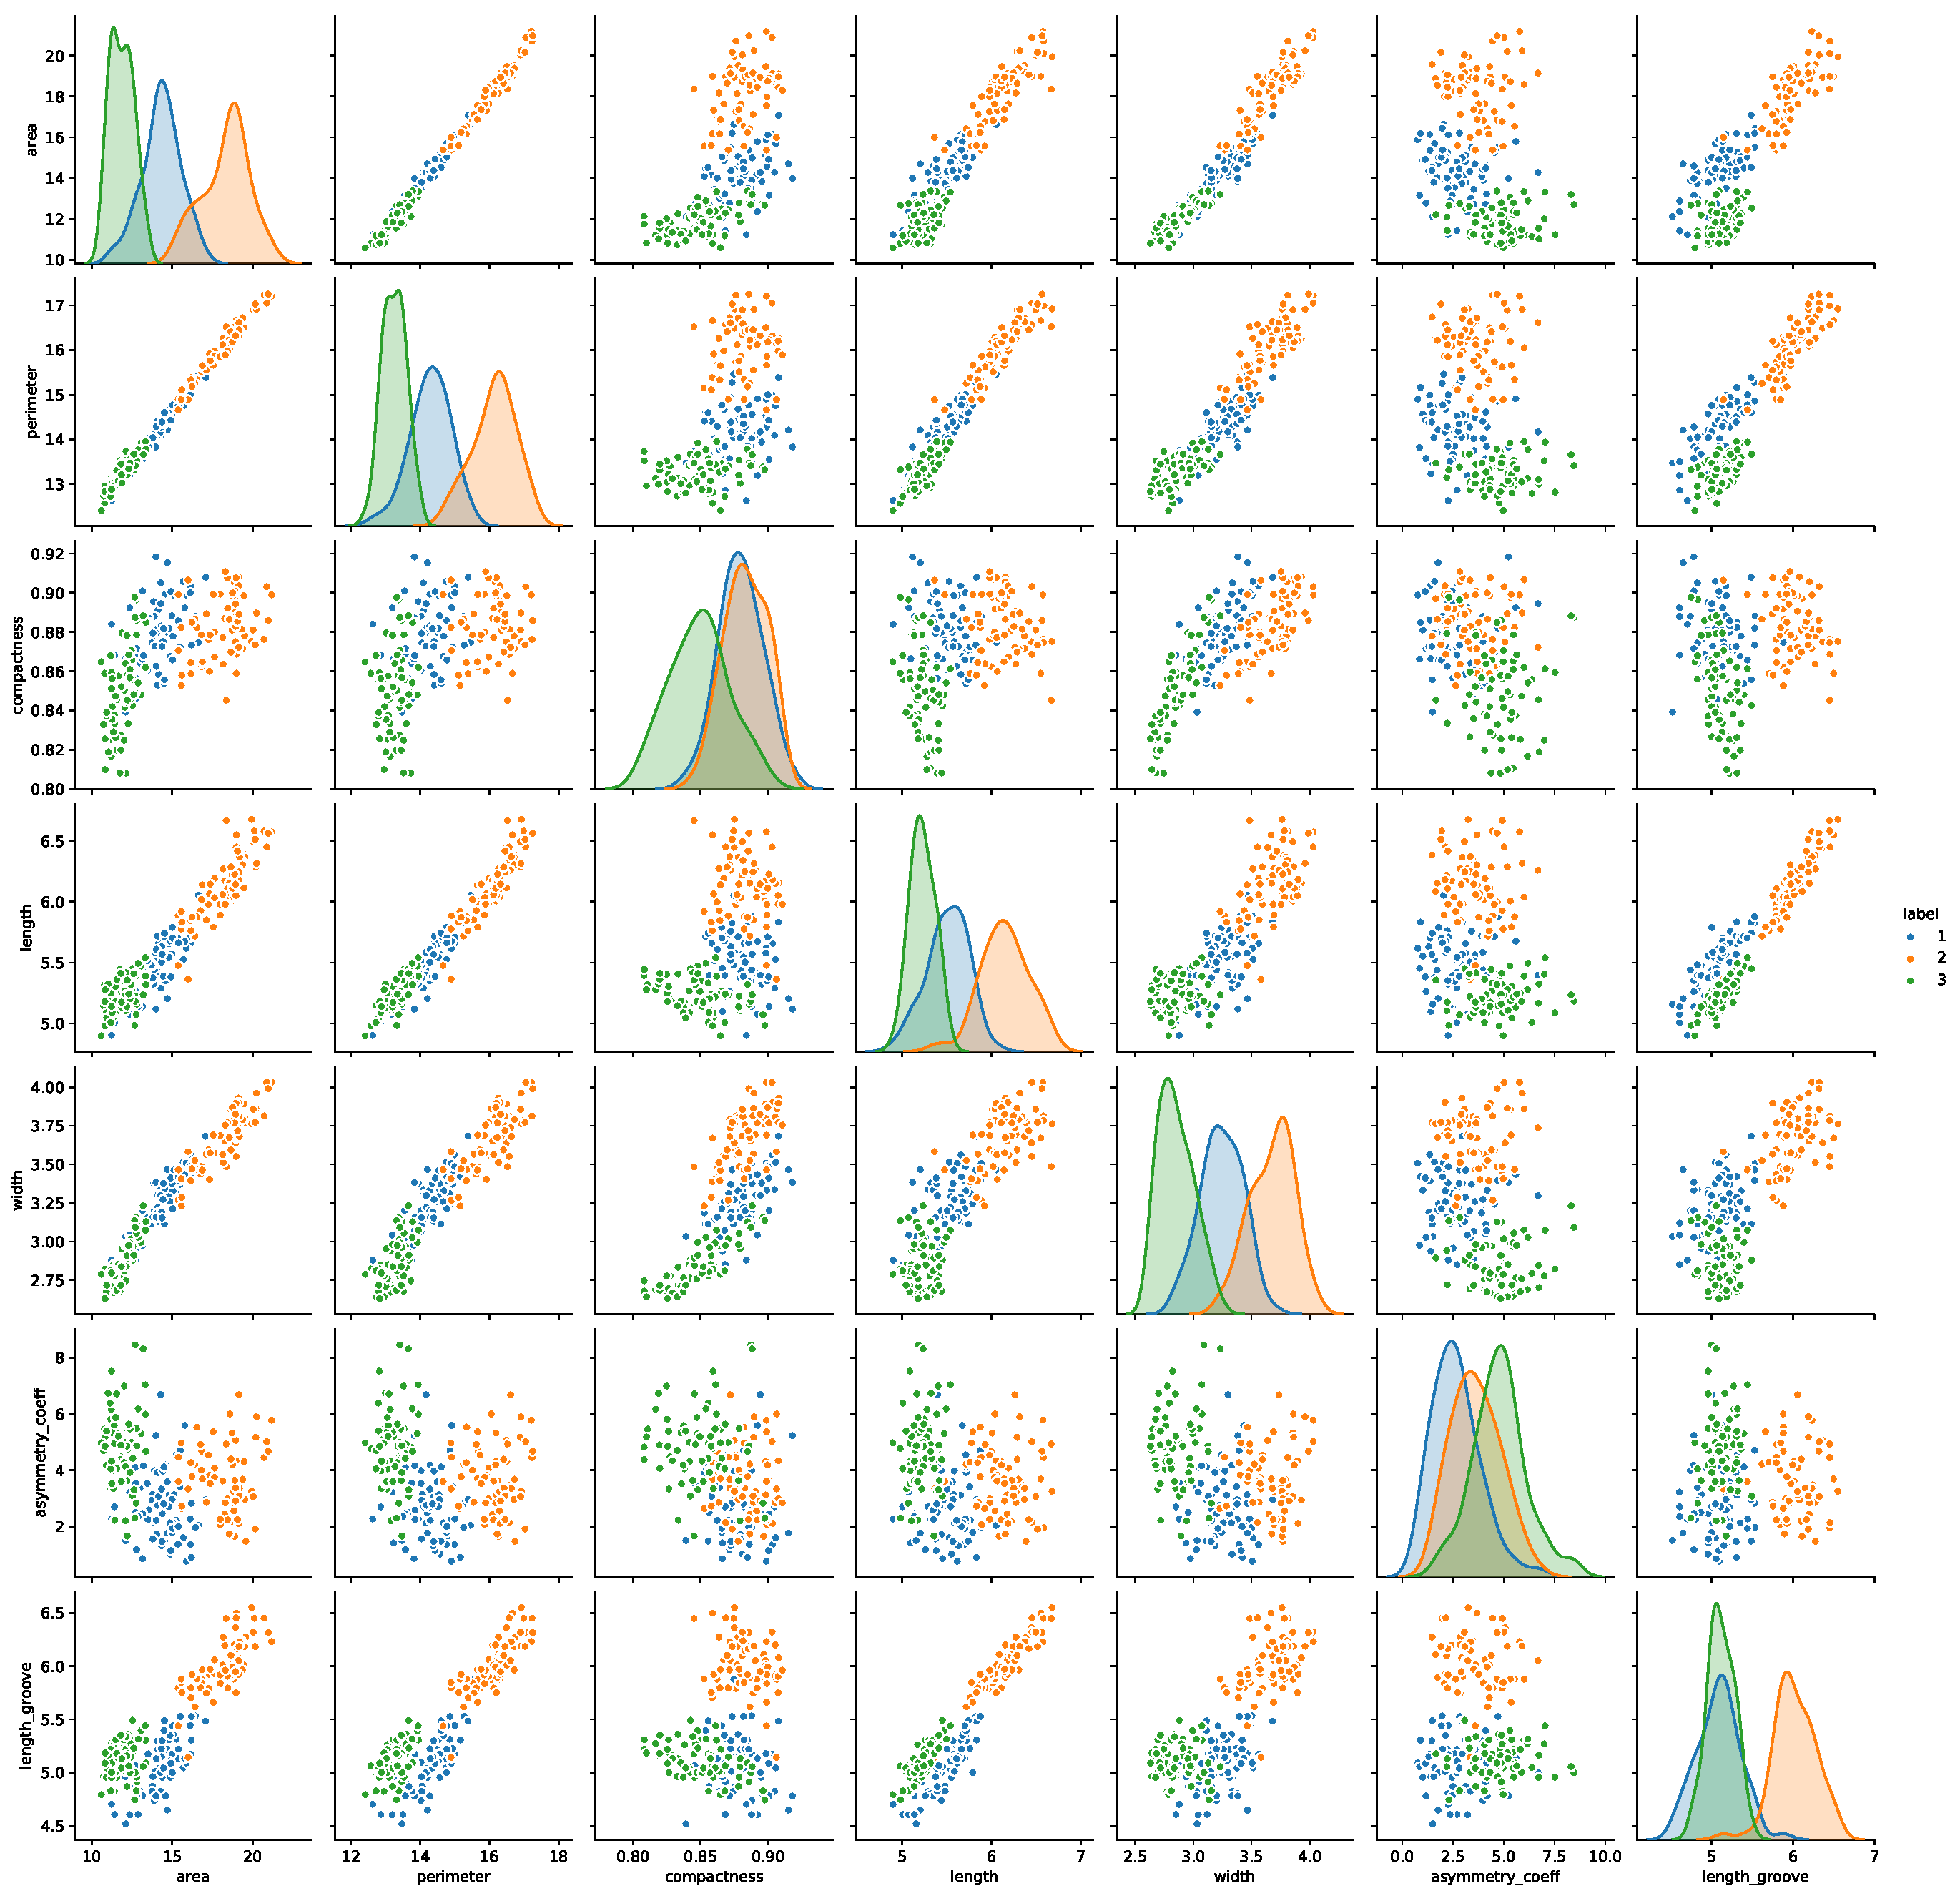
\includepdf[pages=-,scale=.4]{images/seeds_pairplot.pdf}
\begin{center}
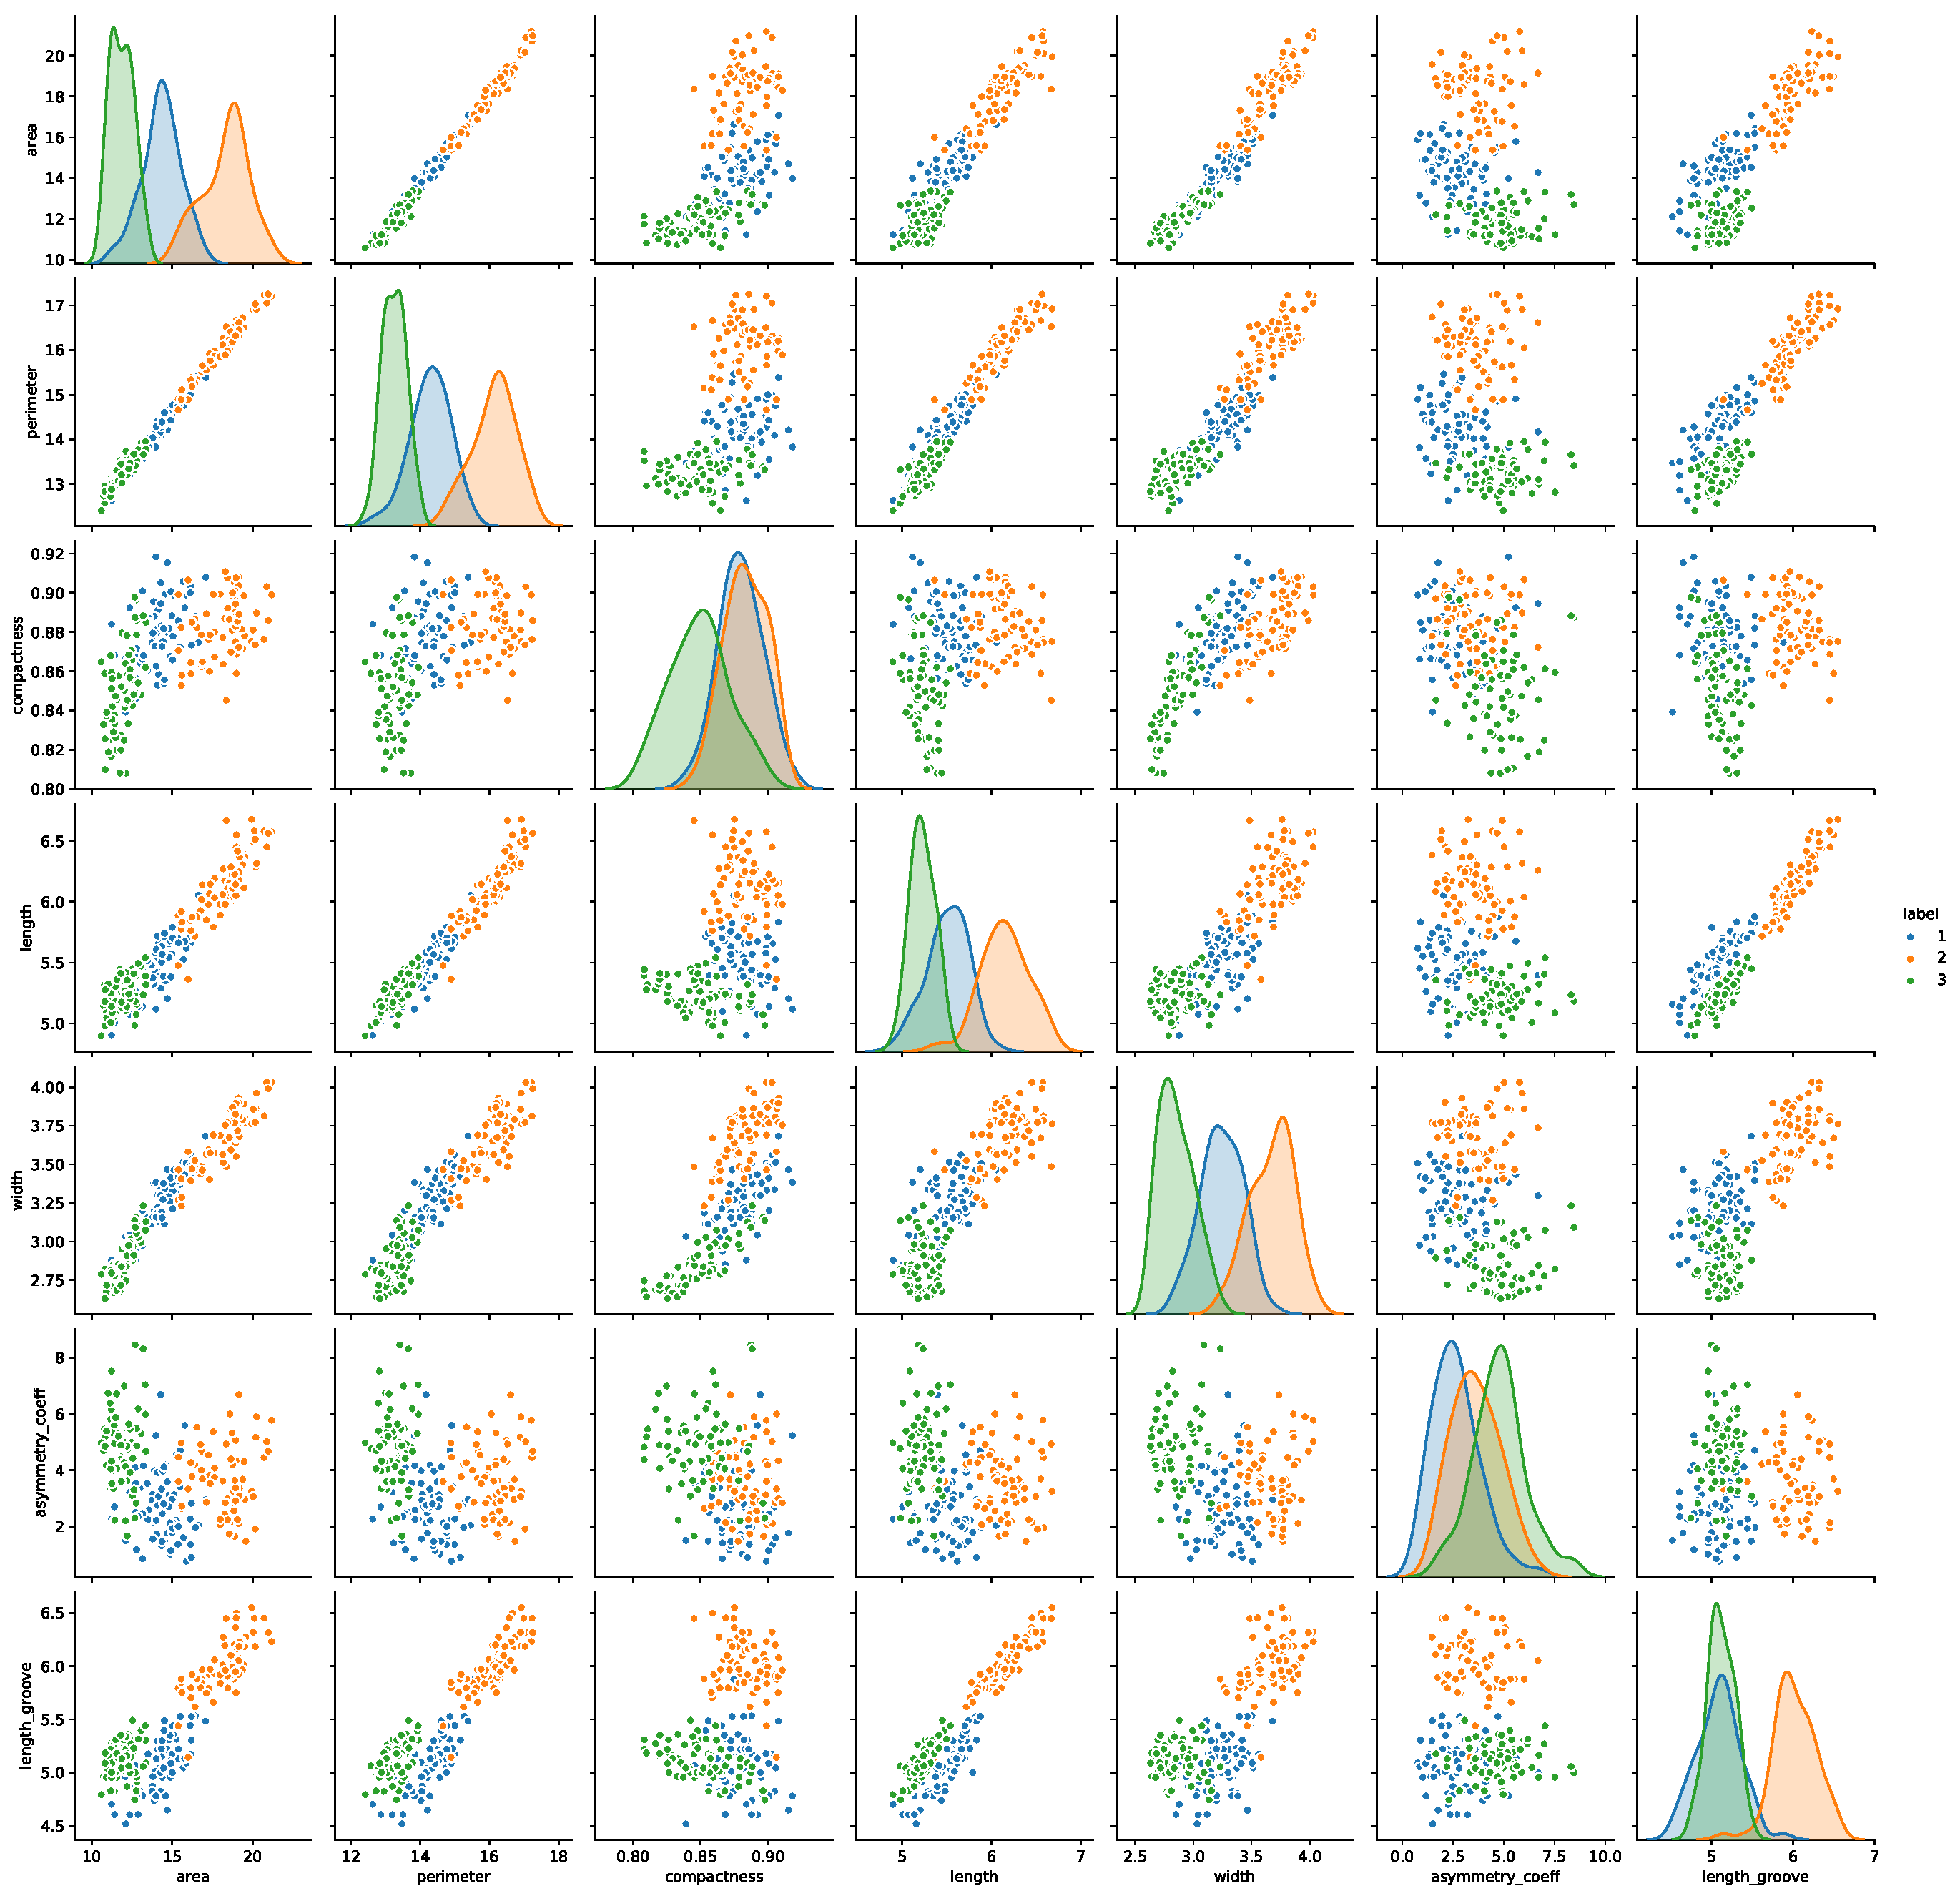
\includegraphics[width=0.75\textwidth]{images/seeds_pairplot.pdf}
\end{center}
\label{img:seeds_pairplot}
\end{figure}

A few things can be noted here: compactness is linearly dependent on two other features in the data set, calling into question what value this information can bring to a clustering method. Furthermore the area is not computed from other measurements, but is highly correlated with width and length and the perimeter. These relationships among others can be seen in figure \ref{img:seeds_pairplot}. Note that these plots have been colored according to their labels. Density plots on the diagonal already show distinct characteristics for the different varieties of kernels for certain features. For the clustering step of course the labels are removed from the data (this data set was included despite not being the typical application of clustering because it can serve as a sort of "control" for the clustering methods when looking at evaluation and conclusions).




\subsection{Red Wine Quality}
\textit{written by M.A.}\\

The data set was used as a wine quality data set and was gathered by Cortez et al. in 2009. It consists of labelled data and contains 11 attributes and 1599 instances. Its goal is to model wine quality based on physicochemical tests \cite{cortez2009modeling}. Due to privacy reasons, only physicochemical (inputs) and sensory (the output - quality) variables are available. That means there is no data about grape types, wine brand, wine selling price, etc..\newline

The input variables are: 
\begin{multicols}{2}
\begin{itemize}
    \item \textit {fixed acidity},
    \item \textit {volatile acidity}, 
    \item \textit {citric acid}, 
    \item \textit {residual sugar},
    \item \textit {chlorides}, 
    \item \textit {free sulfur dioxide}, 
    \item \textit {total sulfur dioxide},
    \item \textit {density}, 
    \item \textit {pH},
    \item \textit {sulphates} and 
    \item \textit {alcohol},
\end{itemize} 
\end{multicols}

which consist of floats and integer values.   \newline

While the \textit {fixed acidity} describes the acids in wine, which are mostly fixed or nonvolatile, the \textit {volatile acidity} describes the amount of acetic acid in wine, which can lead to an unpleasant vinegar taste, when it is too high.  The \textit {citric acid} is found in small quantities and can add freshness and flavor to wines. Its values lie between 0-1. \newline
Additionally, the attribute \textit{residual sugar} comprises the amount of sugar remaining after fermentation stops. It is rare to find wines with less than 1 gram/liter that is why even 15.5 gram/liter is being reached. \newline
\textit {Chlorides} describe the amount of salt in the wine, which is very less, specifically between 0.01 – 0.61. \newline
\textit {Free sulfur dioxides} and \textit {total sulfur dioxides} describe the amount of free and bound forms of SO2. In low concentrations, SO2 is mostly undetectable in wine, but at free SO2 its much easier.
Furthermore, \textit {density} of water is being used to describe wine quality and its values are between 
0.99 and 1. \newline
Additionally, the \textit {pH} value describes how acid or basic a wine is on a scale from 0 (very acid) to 14 (very basic). Most vines are between 3-4. \textit {Sulphates} describe a wine additive.
The last attribute \textit {alcohol} holds details about the percent alcohol content of the wine. 
\textit {Quality} is described as an output variable, which is based on the sensory data. The score is between 0 and 10 \cite{kaggle-redwine}.\newline
This dataset does not include empty columns, nor does it have empty values.
Figure \ref{fig:wine_stats} depicts the spread of each attribute in the pillar chart of the wine quality data set \cite{kaggle-redwine}. This data set is suggested to be used for regression or classification modelling \cite{kaggle-redwine}.
That’s why we have chosen it for clustering. \newline

\begin{figure}[H]
%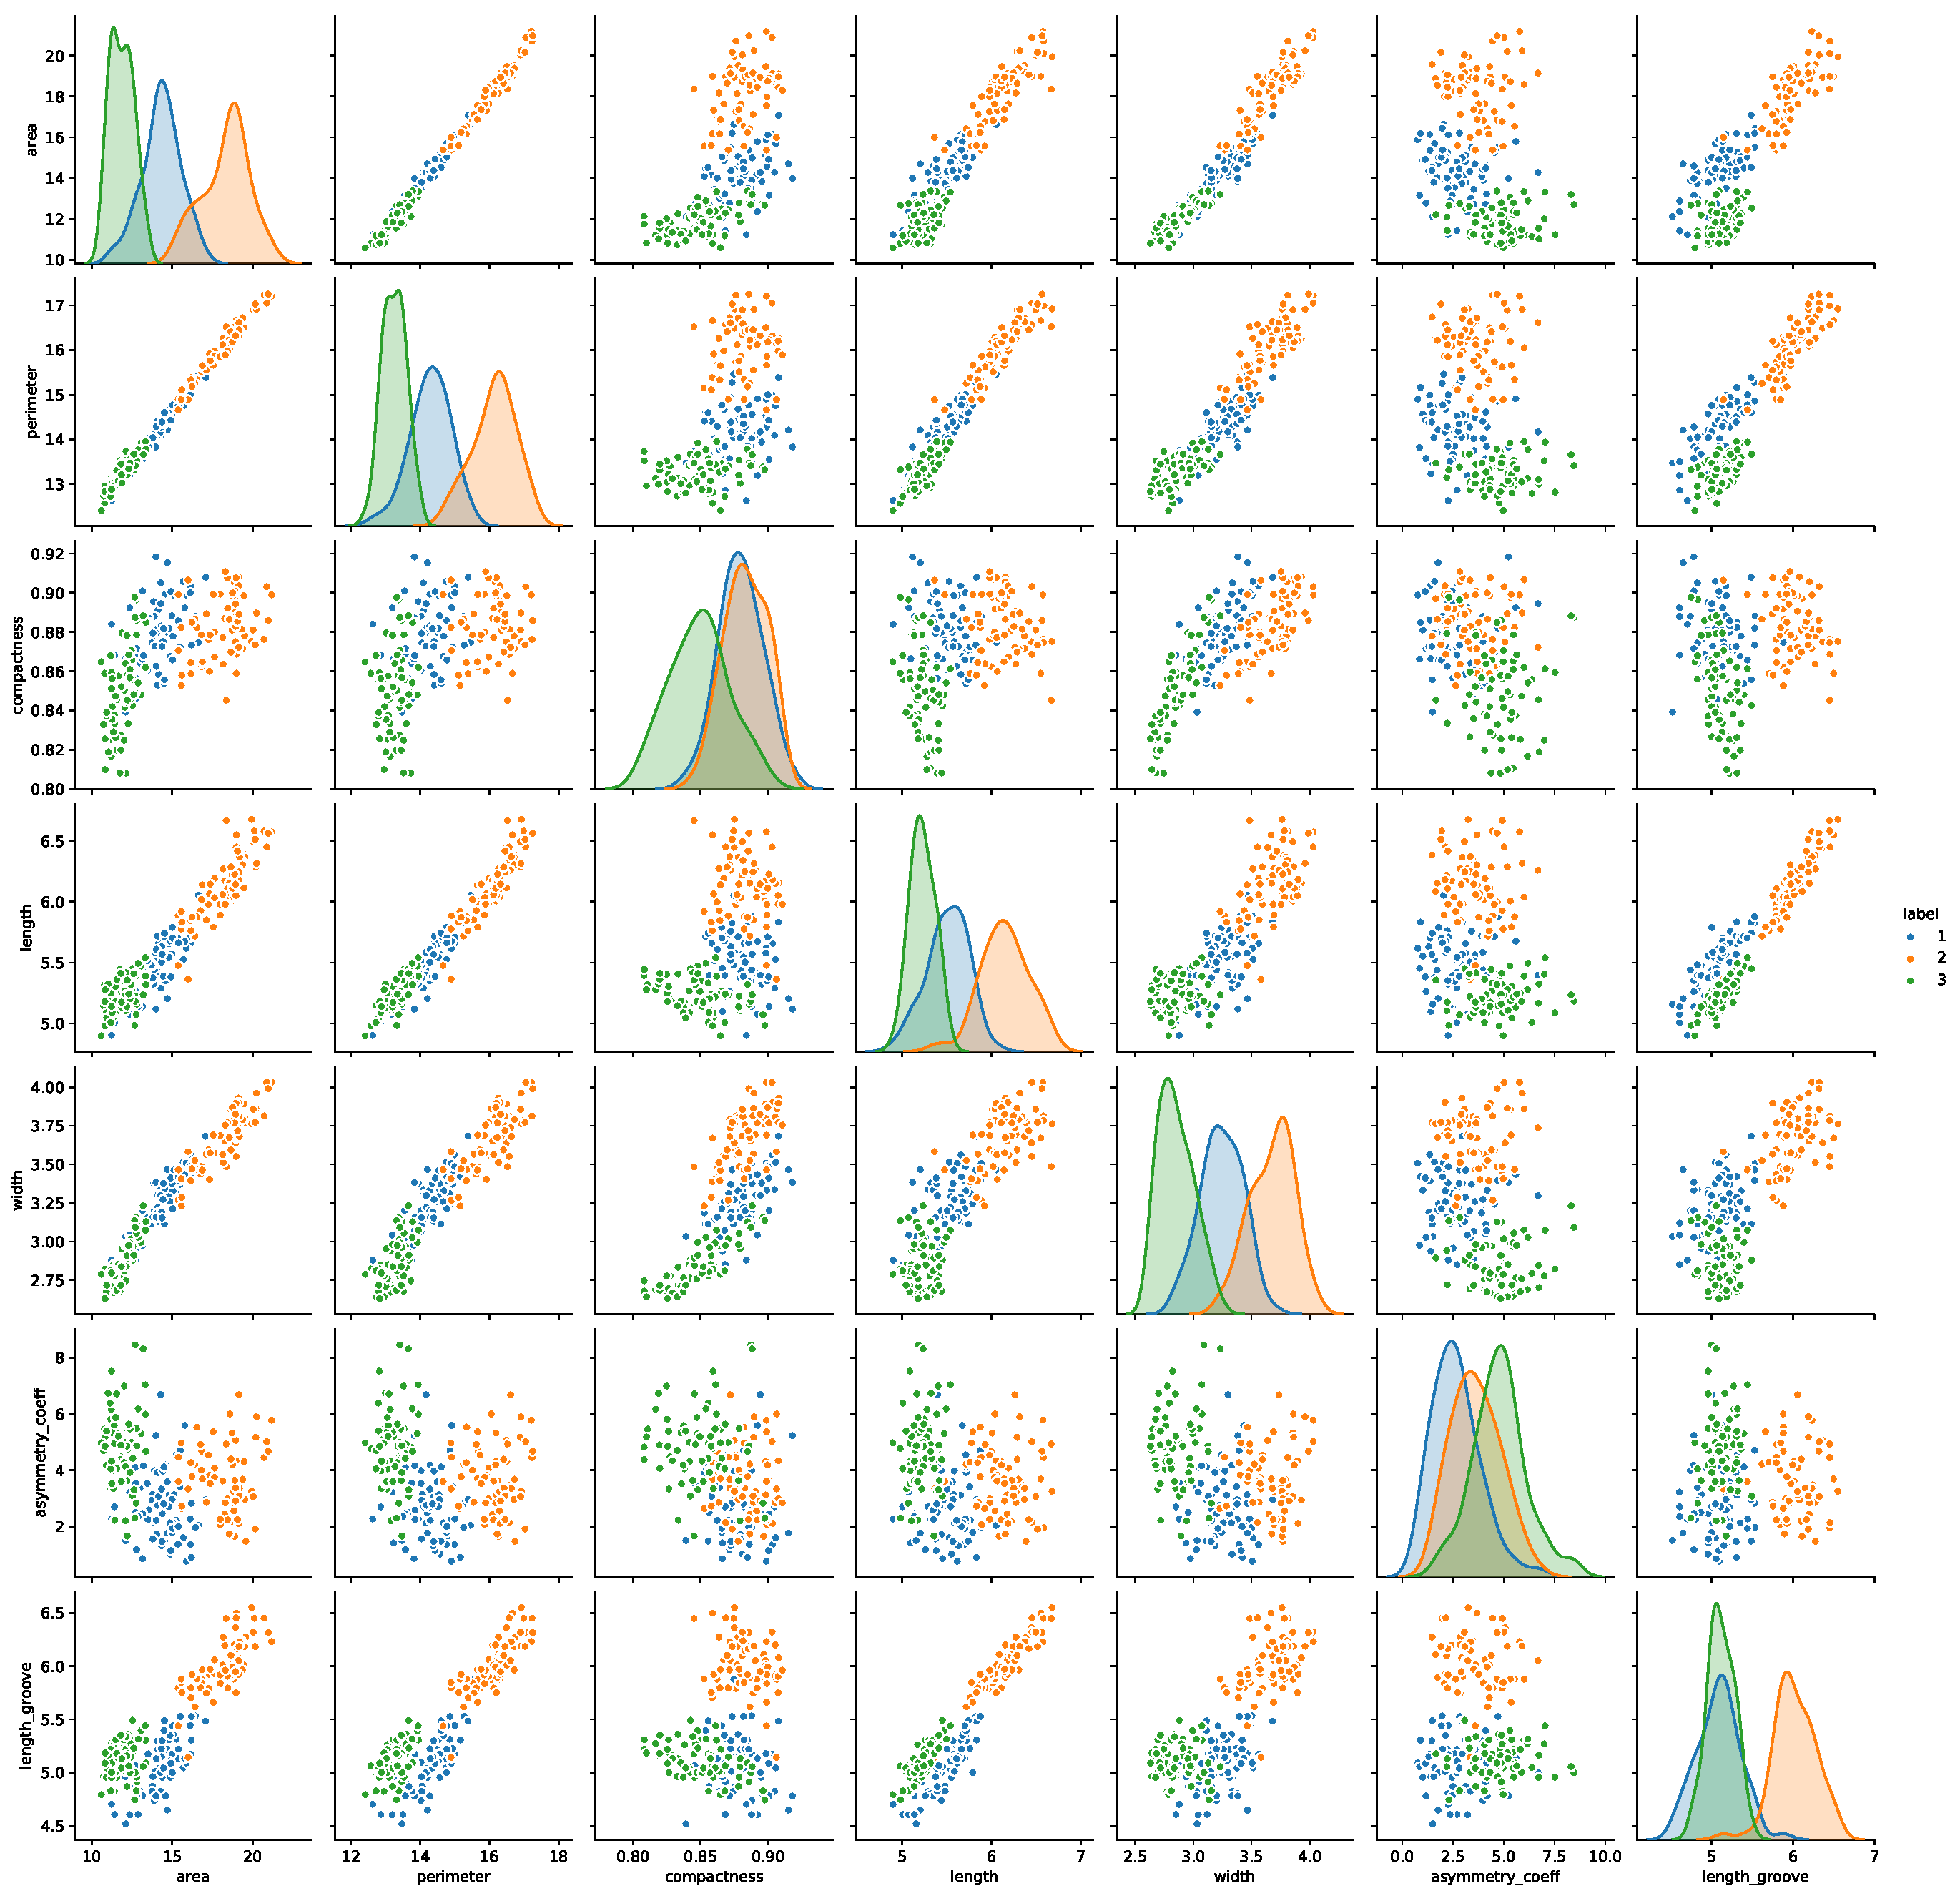
\includepdf[pages=-,scale=.4]{images/seeds_pairplot.pdf}
\centering
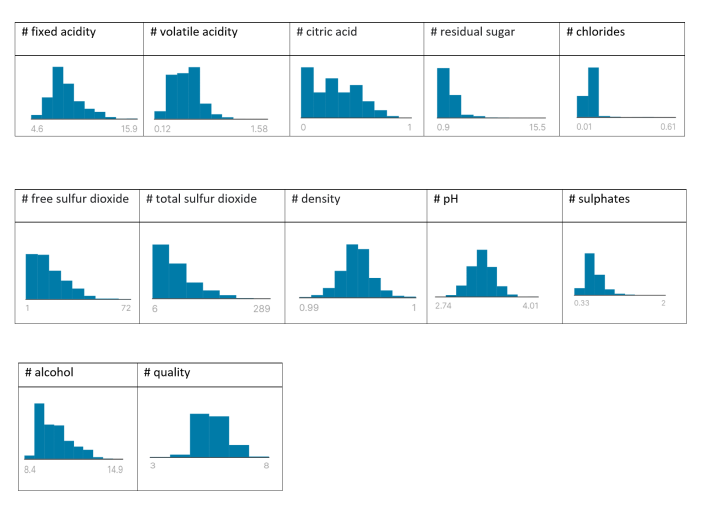
\includegraphics[width=1\textwidth]{images/wine_table.png}
\caption{Spread of each attribute of the wine quality data set}
\label{fig:wine_stats}
\end{figure}

\section{Data Set Description}
\label{sec:data_description}
% \begin{itemize}
% \item What benchmark data sets are used?
% \end{itemize}

\subsection{Boston House Pricing Data}
\textit{written by L.B.}\\

The Boston House Pricing data set was originally published in 1978 by Harrison and Rubinfeld \cite{hedonichousepricing}. In their study the authors used the data set to investigate how people's willingness to pay for clean air is correlated with different measurements of house data around the area of Boston.
In total, 506 samples are included within the data set, containing fourteen different attribute columns. Six of those attribute values originate from the U.S. Census Service, the remaining originate amongst others from the FBI, the Metropolitan Area Planning Commission, the Massachusetts Taxpayers Foundation, the Massachusetts Department of Education and the MIT Boston project. All data was sampled in 1970. The attributes of each data can be separated into different types, providing information on structure, neighborhood, accessibility or air pollution.

Structural attributes yield information on the state of the house with respect to year of construction or spaciousness. While the \textit{RM} variable holds the numeric value for the average number of rooms, the \textit{AGE} attribute describes the proportion of houses that were built before 1940. Both values are assumed to have a positive correlation with housing values since owning more rooms or owning houses with modern structures is perceived as increasing life quality. 

Neighborhood attributes hold details about the socioeconomic status of the environment. This includes the fraction of colored people in the whole population, as well as the \textit{LSTAT} attribute, which denotes the amount of people being of lower educational status. In addition to that, crime rate is included for neighborhoods of Boston area. The latter attribute is supposed to have a negative effect on housing values as crime rate influences people's level of danger. 
Another neighborhood attribute stands for the sum of square feet available for residential zoning where constructing buildings like factories is prohibited. Next, the \textit{INDUS} attribute comprises the proportion of industry which comes along with noise, traffic and dirt and is therefore negatively correlated with housing values. Moreover, property tax rate as well as the ratio between pupils and teachers are included. The last socioeconomic attribute classifies whether the respective city area adjoins Charles River.

Accessibility attributes characterize infrastructure measured by closeness to employment centers and to radial highways. 

In order to estimate air quality, the concentration of Nitrogen Oxid in parts per hundred million is measured. 

The last attribute is the dependent variable which describes the median value of houses that are occupied by private owners. 

While the index of highway accessibility is an integer value and the closeness to Charles River is described using a binary variable encoded as 0 and 1, the remaining attributes are float numbers. The data set does not contain any empty columns, thus no elimination or preprocessing of the available data is necessary.\newline
Table \ref{tab:housing_table} provides some general statistics on the given data set. For each of the columns except the measurement of closeness to Charles River, mean, minimum and maximum value as well as the standard deviation are given. In addition to that, lower (0.25) and upper (0.75) quartiles and the 50\%-quantiles are listed for each of the thirteen features. Quantiles yield information on how the data points are distributed within the high-dimensional feature space. It can be observed that for most of the features, data points lie relatively close together, proposing the data set to consist of dense regions. 

\begin{table}[H]
    \centering
    \begin{tabular}{c|c|c|c|c|c|c|c}
          \hline
         Column & Mean & Min & Max & Std & 25\% & 50\% & 75\%  \\
        \hline
         CRIM & 3.614 & 0.006 & 88.976 & 8.593 & 0.082 & 0.257 & 3.677\\
         ZN & 11.364 & 0.000 & 100.000 & 23.299 & 0.000 & 0.000 & 12.5\\
         INDUS & 11.137 & 0.460 & 27.740 & 6.854 & 5.190 & 9.960 & 18.100\\
         NOX & 0.555 & 0.385 & 0.871 & 0.116 & 0.449 & 0.538 & 0.624\\
         RM & 6.285 & 3.561 & 8.780 & 0.702 & 5.886 & 6.209 & 6.624\\
         AGE & 68.575 & 2.900 & 100.000 & 28.121 & 45.025 & 77.500 & 94.075\\
         DIS & 3.795 & 1.130 & 12.127 & 2.104 & 2.100 & 3.207 & 5.188\\
         RAD & 9.549 & 1.000 & 24.000 & 8.699 & 4.000 & 5.000 & 24.000\\
         TAX & 408.237 & 187.000 & 711.000 & 168.371 & 279.000 & 330.000 & 666.000\\
         PTRATIO & 18.456 & 12.600 & 22.000 & 2.163 & 17.400 & 19.050 & 20.200\\
         B & 356.674 & 0.320 & 396.9 & 91.205 & 375.378 & 391.44 & 396.225\\
         LSTAT & 12.653 & 1.730 & 37.970 & 7.134 & 6.950 & 11.360 & 16.955\\
         MEDV & 22.533 & 5.000 & 50.000 & 9.188 & 17.025 & 21.200 & 25.000\\
    \end{tabular}
    \caption{General Statistics on Boston House Pricing Data Set}
    \label{tab:housing_table}
\end{table}
\subsection{Mall Customer Segmentation}
\textit{by J. M.}\\

The Data Set Mall Customer Segmentation Data includes basic customer data. It contains a unique Id for each customer, gender, age, the annual income, and the spending Score. In this Score you can have a value between 1 and 100. The distribution of gender of the customer is 56\% female and 44 \% male. In the preprocessing every entry of the gender column gets a number 0 or 1 depending on the gender is male or female. I do this because than every entry of this dataset contains only numbers. The Age of the Customers is between 18 und 70. The Annual Income of the customers is between 15 and 127. 
\subsection{Seeds Data}

This data set has been used in the work of \cite{charytanowicz2010complete}. The data comprises information on different features of wheat kernels. There are seven species with a total of about 20 varieties of which three can be found in the data: Kama, Rosa and Canadian wheat. There is a total of 210 data points, evenly split between the varieties. The kernels for which data was collected were selected randomly. They were then examined through X-ray imaging. A software called \textit{GRAINS} for this specific application \cite{strumillo1999computer} was used to extract the features for each observation:
\begin{multicols}{2}
\begin{itemize}
\item area $A$
\item perimeter $P$
\item compactness $C = 4 \pi A/P^{2}$
\item length (along groove)
\item width
\item asymmetry coefficient
\item length of kernel groove
\item label
\end{itemize}
\end{multicols}

\begin{figure}[h]
\caption{Seeds pairplot WIP}
%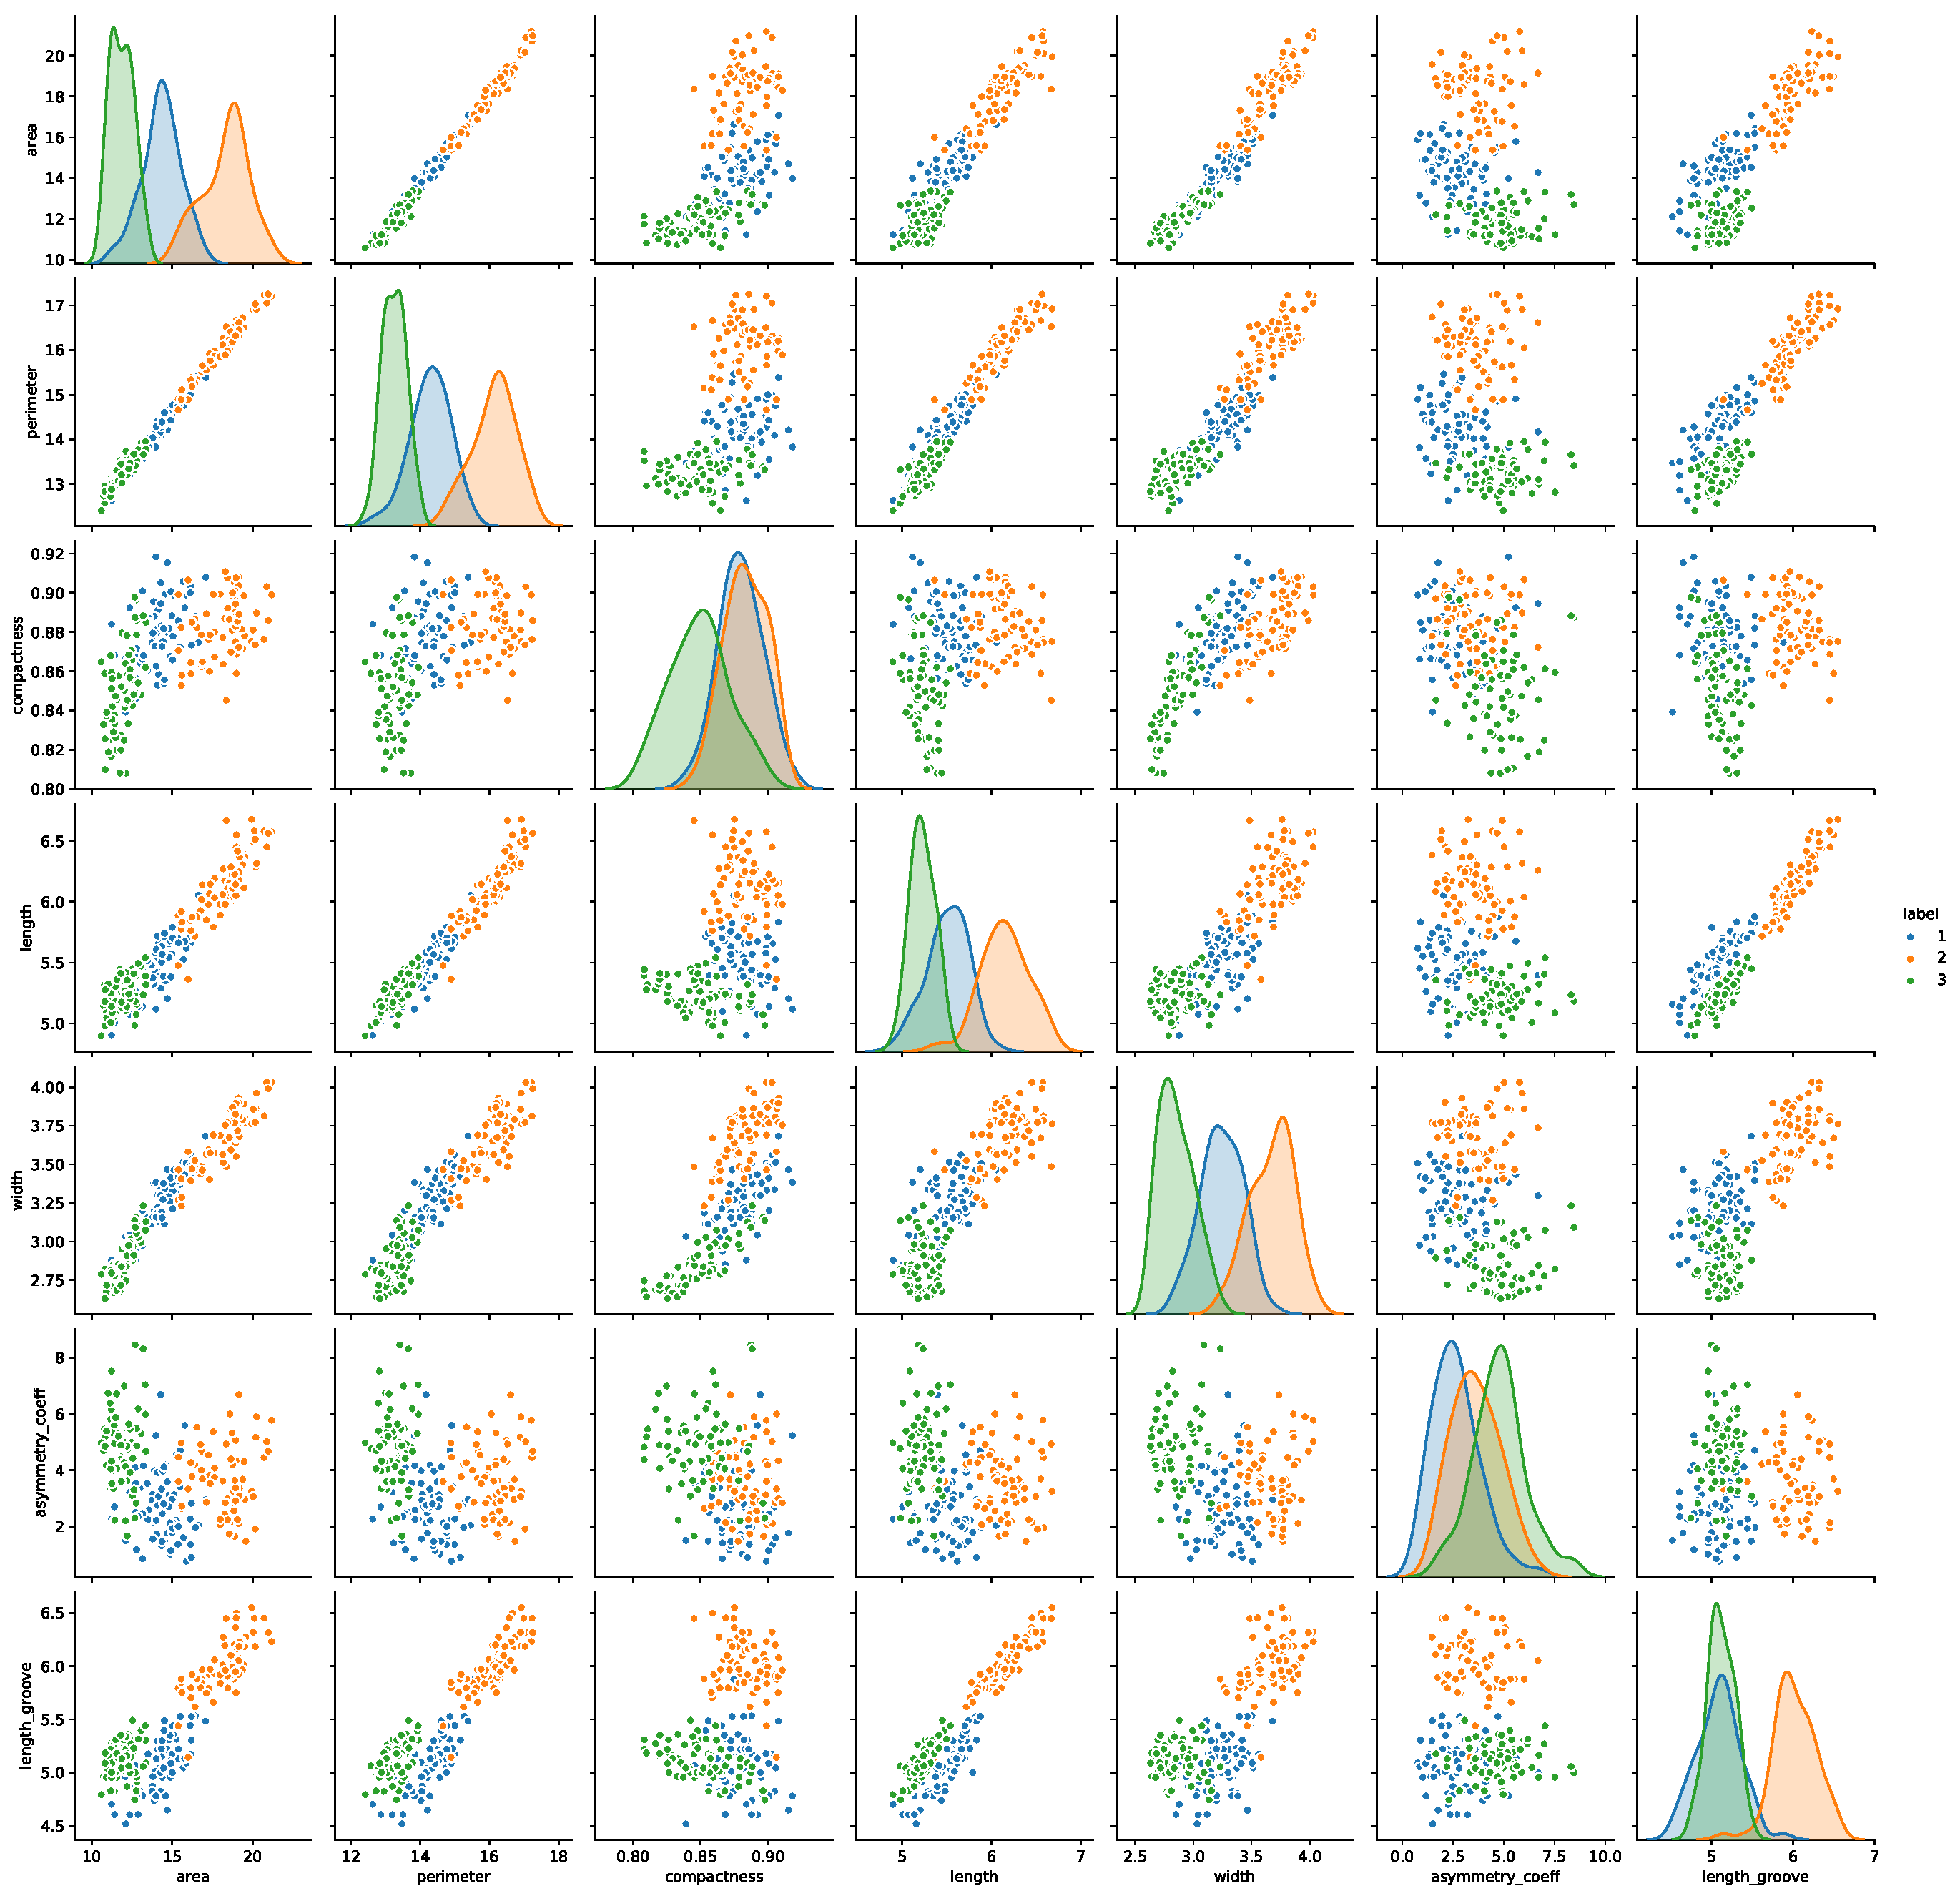
\includepdf[pages=-,scale=.4]{images/seeds_pairplot.pdf}
\begin{center}
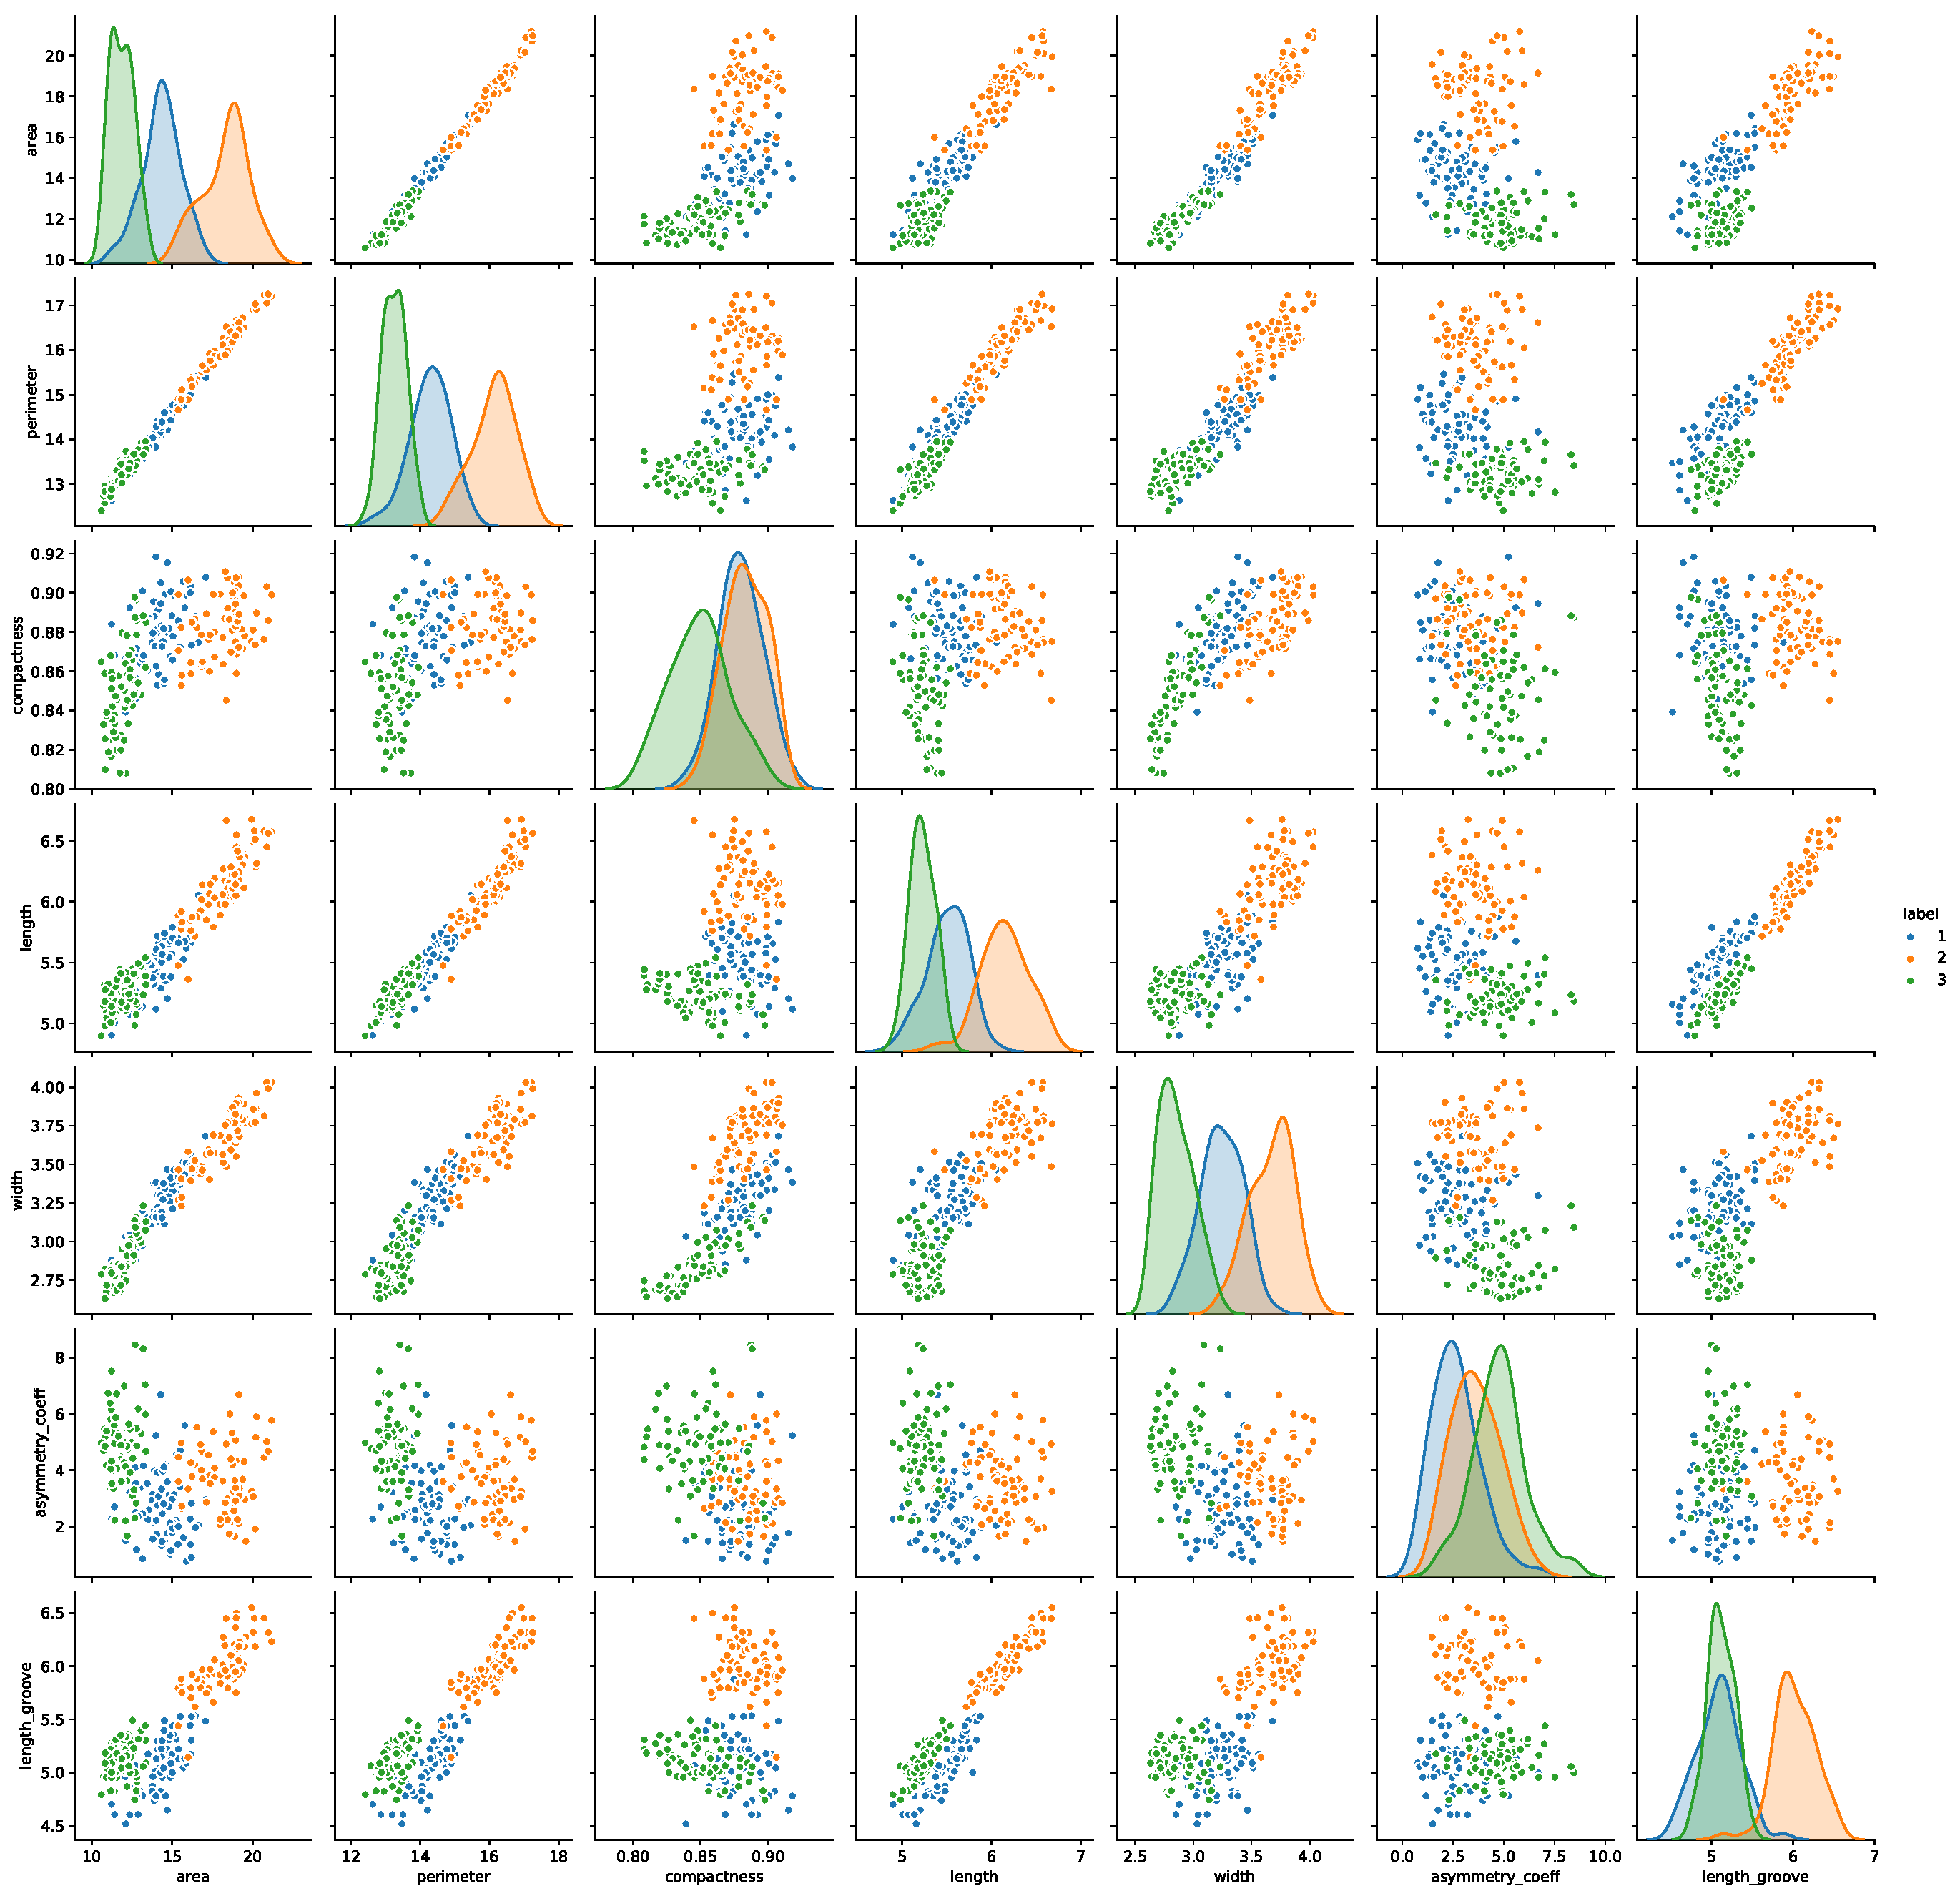
\includegraphics[width=0.75\textwidth]{images/seeds_pairplot.pdf}
\end{center}
\label{img:seeds_pairplot}
\end{figure}

A few things can be noted here: compactness is linearly dependent on two other features in the data set, calling into question what value this information can bring to a clustering method. Furthermore the area is not computed from other measurements, but is highly correlated with width and length and the perimeter. These relationships among others can be seen in figure \ref{img:seeds_pairplot}. Note that these plots have been colored according to their labels. Density plots on the diagonal already show distinct characteristics for the different varieties of kernels for certain features. For the clustering step of course the labels are removed from the data (this data set was included despite not being the typical application of clustering because it can serve as a sort of "control" for the clustering methods when looking at evaluation and conclusions).




\subsection{Red Wine Quality}
\textit{written by M.A.}\\

The data set was used as a wine quality data set and was gathered by Cortez et al. in 2009. It consists of labelled data and contains 11 attributes and 1599 instances. Its goal is to model wine quality based on physicochemical tests \cite{cortez2009modeling}. Due to privacy reasons, only physicochemical (inputs) and sensory (the output - quality) variables are available. That means there is no data about grape types, wine brand, wine selling price, etc..\newline

The input variables are: 
\begin{multicols}{2}
\begin{itemize}
    \item \textit {fixed acidity},
    \item \textit {volatile acidity}, 
    \item \textit {citric acid}, 
    \item \textit {residual sugar},
    \item \textit {chlorides}, 
    \item \textit {free sulfur dioxide}, 
    \item \textit {total sulfur dioxide},
    \item \textit {density}, 
    \item \textit {pH},
    \item \textit {sulphates} and 
    \item \textit {alcohol},
\end{itemize} 
\end{multicols}

which consist of floats and integer values.   \newline

While the \textit {fixed acidity} describes the acids in wine, which are mostly fixed or nonvolatile, the \textit {volatile acidity} describes the amount of acetic acid in wine, which can lead to an unpleasant vinegar taste, when it is too high.  The \textit {citric acid} is found in small quantities and can add freshness and flavor to wines. Its values lie between 0-1. \newline
Additionally, the attribute \textit{residual sugar} comprises the amount of sugar remaining after fermentation stops. It is rare to find wines with less than 1 gram/liter that is why even 15.5 gram/liter is being reached. \newline
\textit {Chlorides} describe the amount of salt in the wine, which is very less, specifically between 0.01 – 0.61. \newline
\textit {Free sulfur dioxides} and \textit {total sulfur dioxides} describe the amount of free and bound forms of SO2. In low concentrations, SO2 is mostly undetectable in wine, but at free SO2 its much easier.
Furthermore, \textit {density} of water is being used to describe wine quality and its values are between 
0.99 and 1. \newline
Additionally, the \textit {pH} value describes how acid or basic a wine is on a scale from 0 (very acid) to 14 (very basic). Most vines are between 3-4. \textit {Sulphates} describe a wine additive.
The last attribute \textit {alcohol} holds details about the percent alcohol content of the wine. 
\textit {Quality} is described as an output variable, which is based on the sensory data. The score is between 0 and 10 \cite{kaggle-redwine}.\newline
This dataset does not include empty columns, nor does it have empty values.
Figure \ref{fig:wine_stats} depicts the spread of each attribute in the pillar chart of the wine quality data set \cite{kaggle-redwine}. This data set is suggested to be used for regression or classification modelling \cite{kaggle-redwine}.
That’s why we have chosen it for clustering. \newline

\begin{figure}[H]
%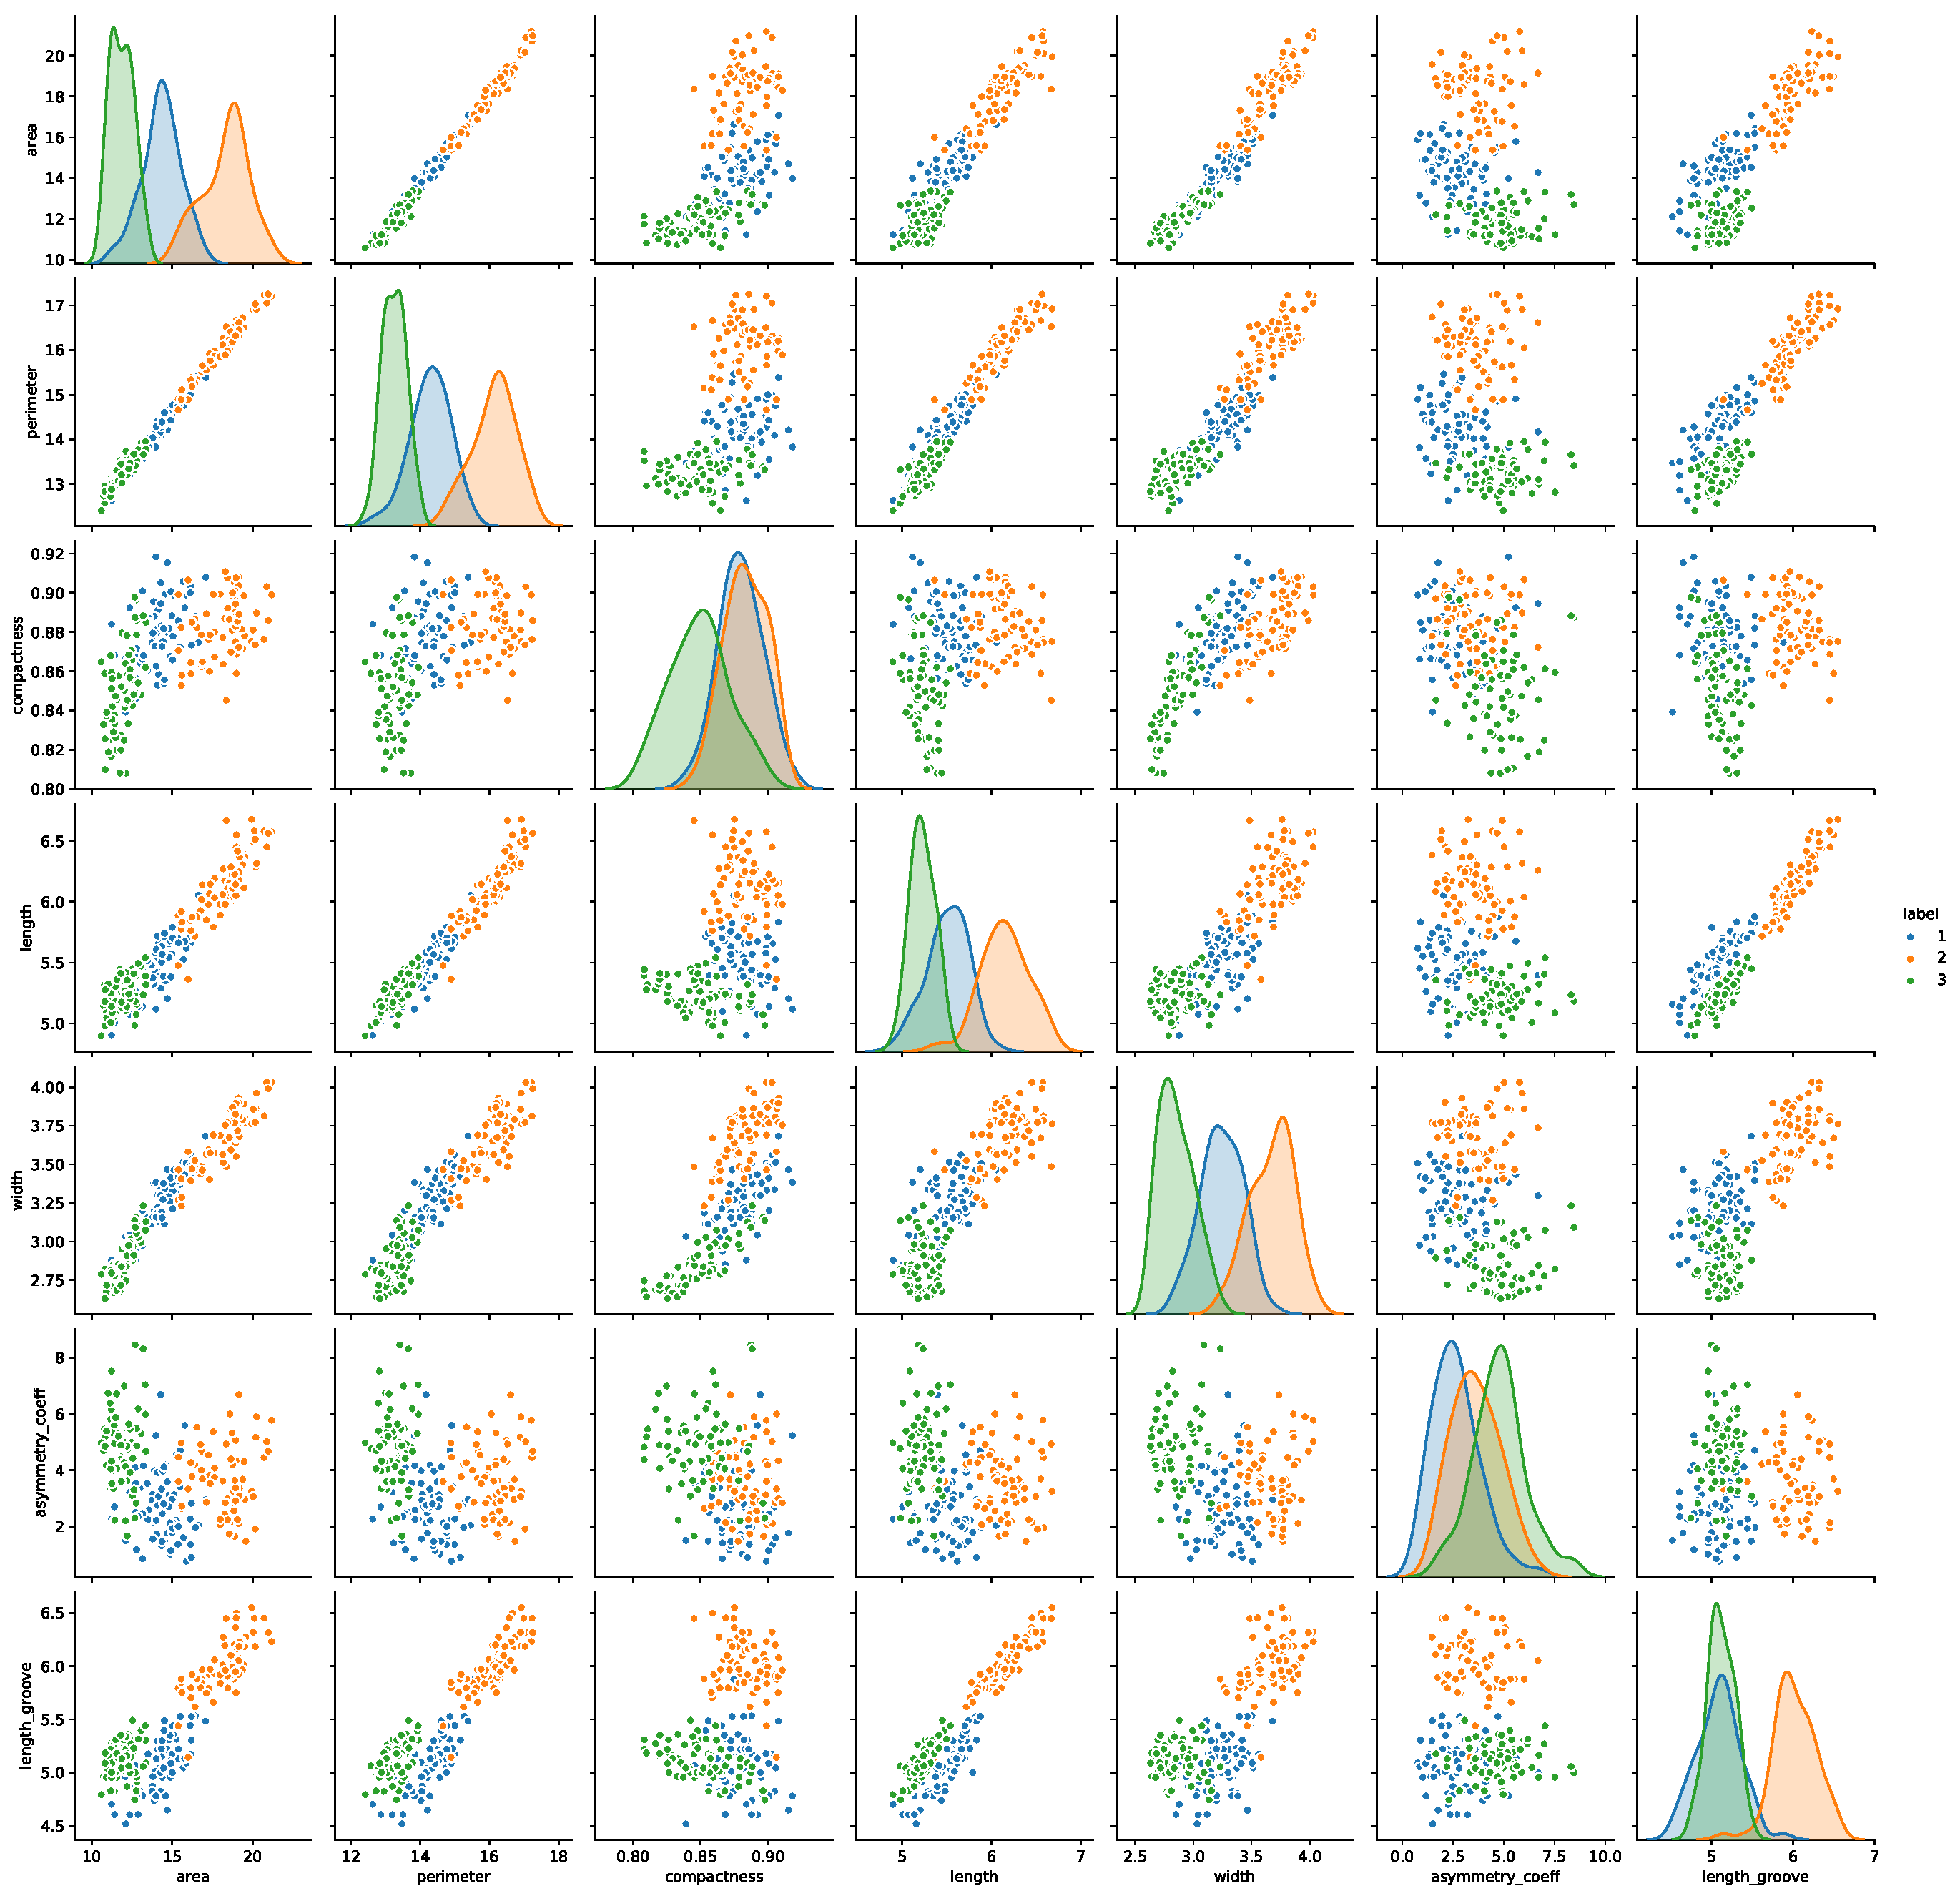
\includepdf[pages=-,scale=.4]{images/seeds_pairplot.pdf}
\centering
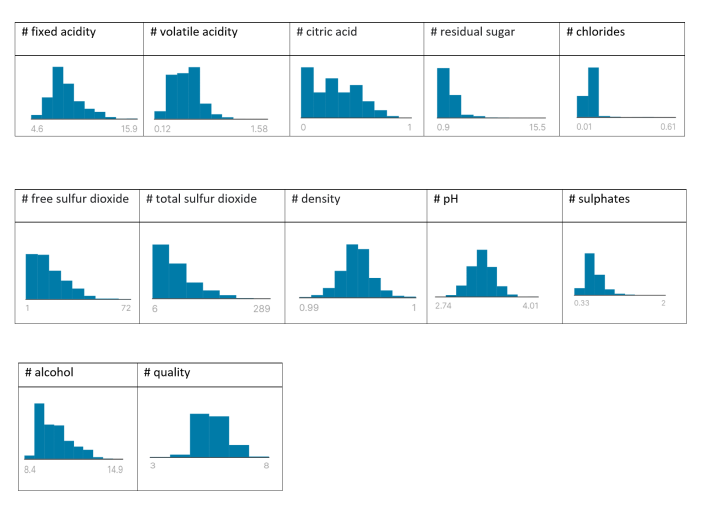
\includegraphics[width=1\textwidth]{images/wine_table.png}
\caption{Spread of each attribute of the wine quality data set}
\label{fig:wine_stats}
\end{figure}

\section{Description of Python libraries used}
\label{sec:python_description}
% \begin{itemize}
% \item What benchmark data sets are used?
% \end{itemize}

\subsection{Boston House Pricing Data}
\textit{written by L.B.}\\

The Boston House Pricing data set was originally published in 1978 by Harrison and Rubinfeld \cite{hedonichousepricing}. In their study the authors used the data set to investigate how people's willingness to pay for clean air is correlated with different measurements of house data around the area of Boston.
In total, 506 samples are included within the data set, containing fourteen different attribute columns. Six of those attribute values originate from the U.S. Census Service, the remaining originate amongst others from the FBI, the Metropolitan Area Planning Commission, the Massachusetts Taxpayers Foundation, the Massachusetts Department of Education and the MIT Boston project. All data was sampled in 1970. The attributes of each data can be separated into different types, providing information on structure, neighborhood, accessibility or air pollution.

Structural attributes yield information on the state of the house with respect to year of construction or spaciousness. While the \textit{RM} variable holds the numeric value for the average number of rooms, the \textit{AGE} attribute describes the proportion of houses that were built before 1940. Both values are assumed to have a positive correlation with housing values since owning more rooms or owning houses with modern structures is perceived as increasing life quality. 

Neighborhood attributes hold details about the socioeconomic status of the environment. This includes the fraction of colored people in the whole population, as well as the \textit{LSTAT} attribute, which denotes the amount of people being of lower educational status. In addition to that, crime rate is included for neighborhoods of Boston area. The latter attribute is supposed to have a negative effect on housing values as crime rate influences people's level of danger. 
Another neighborhood attribute stands for the sum of square feet available for residential zoning where constructing buildings like factories is prohibited. Next, the \textit{INDUS} attribute comprises the proportion of industry which comes along with noise, traffic and dirt and is therefore negatively correlated with housing values. Moreover, property tax rate as well as the ratio between pupils and teachers are included. The last socioeconomic attribute classifies whether the respective city area adjoins Charles River.

Accessibility attributes characterize infrastructure measured by closeness to employment centers and to radial highways. 

In order to estimate air quality, the concentration of Nitrogen Oxid in parts per hundred million is measured. 

The last attribute is the dependent variable which describes the median value of houses that are occupied by private owners. 

While the index of highway accessibility is an integer value and the closeness to Charles River is described using a binary variable encoded as 0 and 1, the remaining attributes are float numbers. The data set does not contain any empty columns, thus no elimination or preprocessing of the available data is necessary.\newline
Table \ref{tab:housing_table} provides some general statistics on the given data set. For each of the columns except the measurement of closeness to Charles River, mean, minimum and maximum value as well as the standard deviation are given. In addition to that, lower (0.25) and upper (0.75) quartiles and the 50\%-quantiles are listed for each of the thirteen features. Quantiles yield information on how the data points are distributed within the high-dimensional feature space. It can be observed that for most of the features, data points lie relatively close together, proposing the data set to consist of dense regions. 

\begin{table}[H]
    \centering
    \begin{tabular}{c|c|c|c|c|c|c|c}
          \hline
         Column & Mean & Min & Max & Std & 25\% & 50\% & 75\%  \\
        \hline
         CRIM & 3.614 & 0.006 & 88.976 & 8.593 & 0.082 & 0.257 & 3.677\\
         ZN & 11.364 & 0.000 & 100.000 & 23.299 & 0.000 & 0.000 & 12.5\\
         INDUS & 11.137 & 0.460 & 27.740 & 6.854 & 5.190 & 9.960 & 18.100\\
         NOX & 0.555 & 0.385 & 0.871 & 0.116 & 0.449 & 0.538 & 0.624\\
         RM & 6.285 & 3.561 & 8.780 & 0.702 & 5.886 & 6.209 & 6.624\\
         AGE & 68.575 & 2.900 & 100.000 & 28.121 & 45.025 & 77.500 & 94.075\\
         DIS & 3.795 & 1.130 & 12.127 & 2.104 & 2.100 & 3.207 & 5.188\\
         RAD & 9.549 & 1.000 & 24.000 & 8.699 & 4.000 & 5.000 & 24.000\\
         TAX & 408.237 & 187.000 & 711.000 & 168.371 & 279.000 & 330.000 & 666.000\\
         PTRATIO & 18.456 & 12.600 & 22.000 & 2.163 & 17.400 & 19.050 & 20.200\\
         B & 356.674 & 0.320 & 396.9 & 91.205 & 375.378 & 391.44 & 396.225\\
         LSTAT & 12.653 & 1.730 & 37.970 & 7.134 & 6.950 & 11.360 & 16.955\\
         MEDV & 22.533 & 5.000 & 50.000 & 9.188 & 17.025 & 21.200 & 25.000\\
    \end{tabular}
    \caption{General Statistics on Boston House Pricing Data Set}
    \label{tab:housing_table}
\end{table}
\subsection{Mall Customer Segmentation}
\textit{by J. M.}\\

The Data Set Mall Customer Segmentation Data includes basic customer data. It contains a unique Id for each customer, gender, age, the annual income, and the spending Score. In this Score you can have a value between 1 and 100. The distribution of gender of the customer is 56\% female and 44 \% male. In the preprocessing every entry of the gender column gets a number 0 or 1 depending on the gender is male or female. I do this because than every entry of this dataset contains only numbers. The Age of the Customers is between 18 und 70. The Annual Income of the customers is between 15 and 127. 
\subsection{Seeds Data}

This data set has been used in the work of \cite{charytanowicz2010complete}. The data comprises information on different features of wheat kernels. There are seven species with a total of about 20 varieties of which three can be found in the data: Kama, Rosa and Canadian wheat. There is a total of 210 data points, evenly split between the varieties. The kernels for which data was collected were selected randomly. They were then examined through X-ray imaging. A software called \textit{GRAINS} for this specific application \cite{strumillo1999computer} was used to extract the features for each observation:
\begin{multicols}{2}
\begin{itemize}
\item area $A$
\item perimeter $P$
\item compactness $C = 4 \pi A/P^{2}$
\item length (along groove)
\item width
\item asymmetry coefficient
\item length of kernel groove
\item label
\end{itemize}
\end{multicols}

\begin{figure}[h]
\caption{Seeds pairplot WIP}
%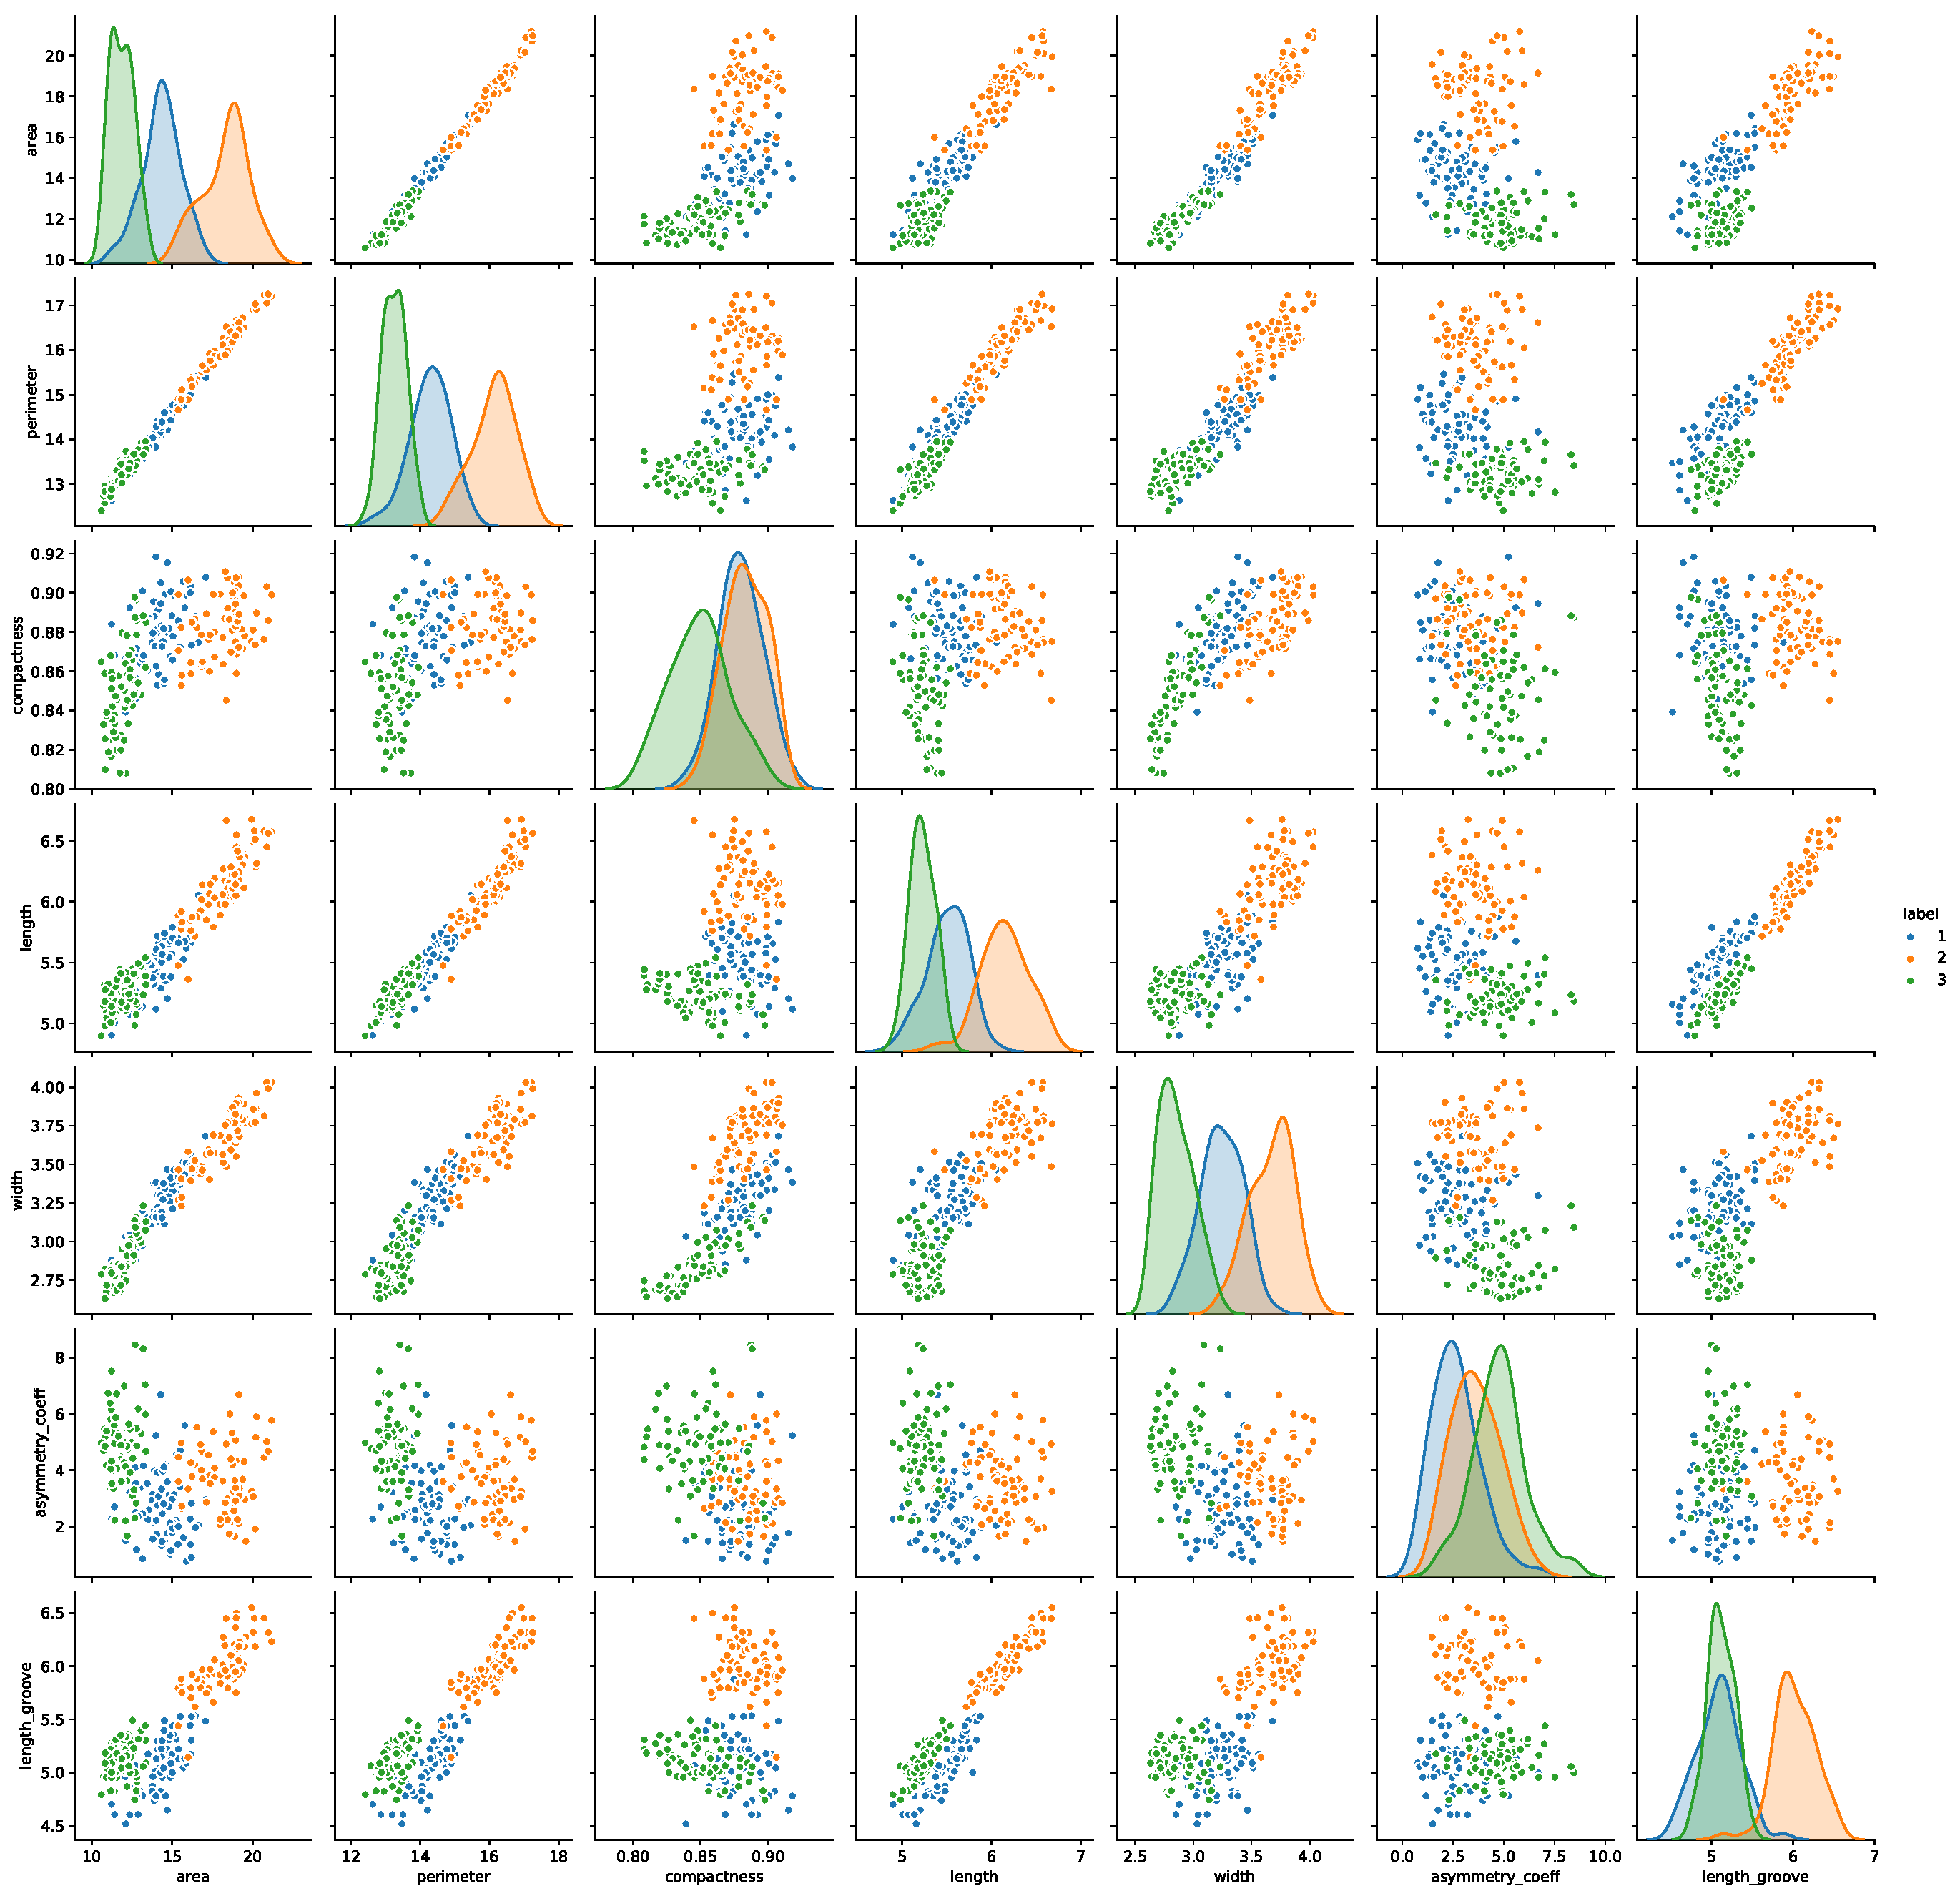
\includepdf[pages=-,scale=.4]{images/seeds_pairplot.pdf}
\begin{center}
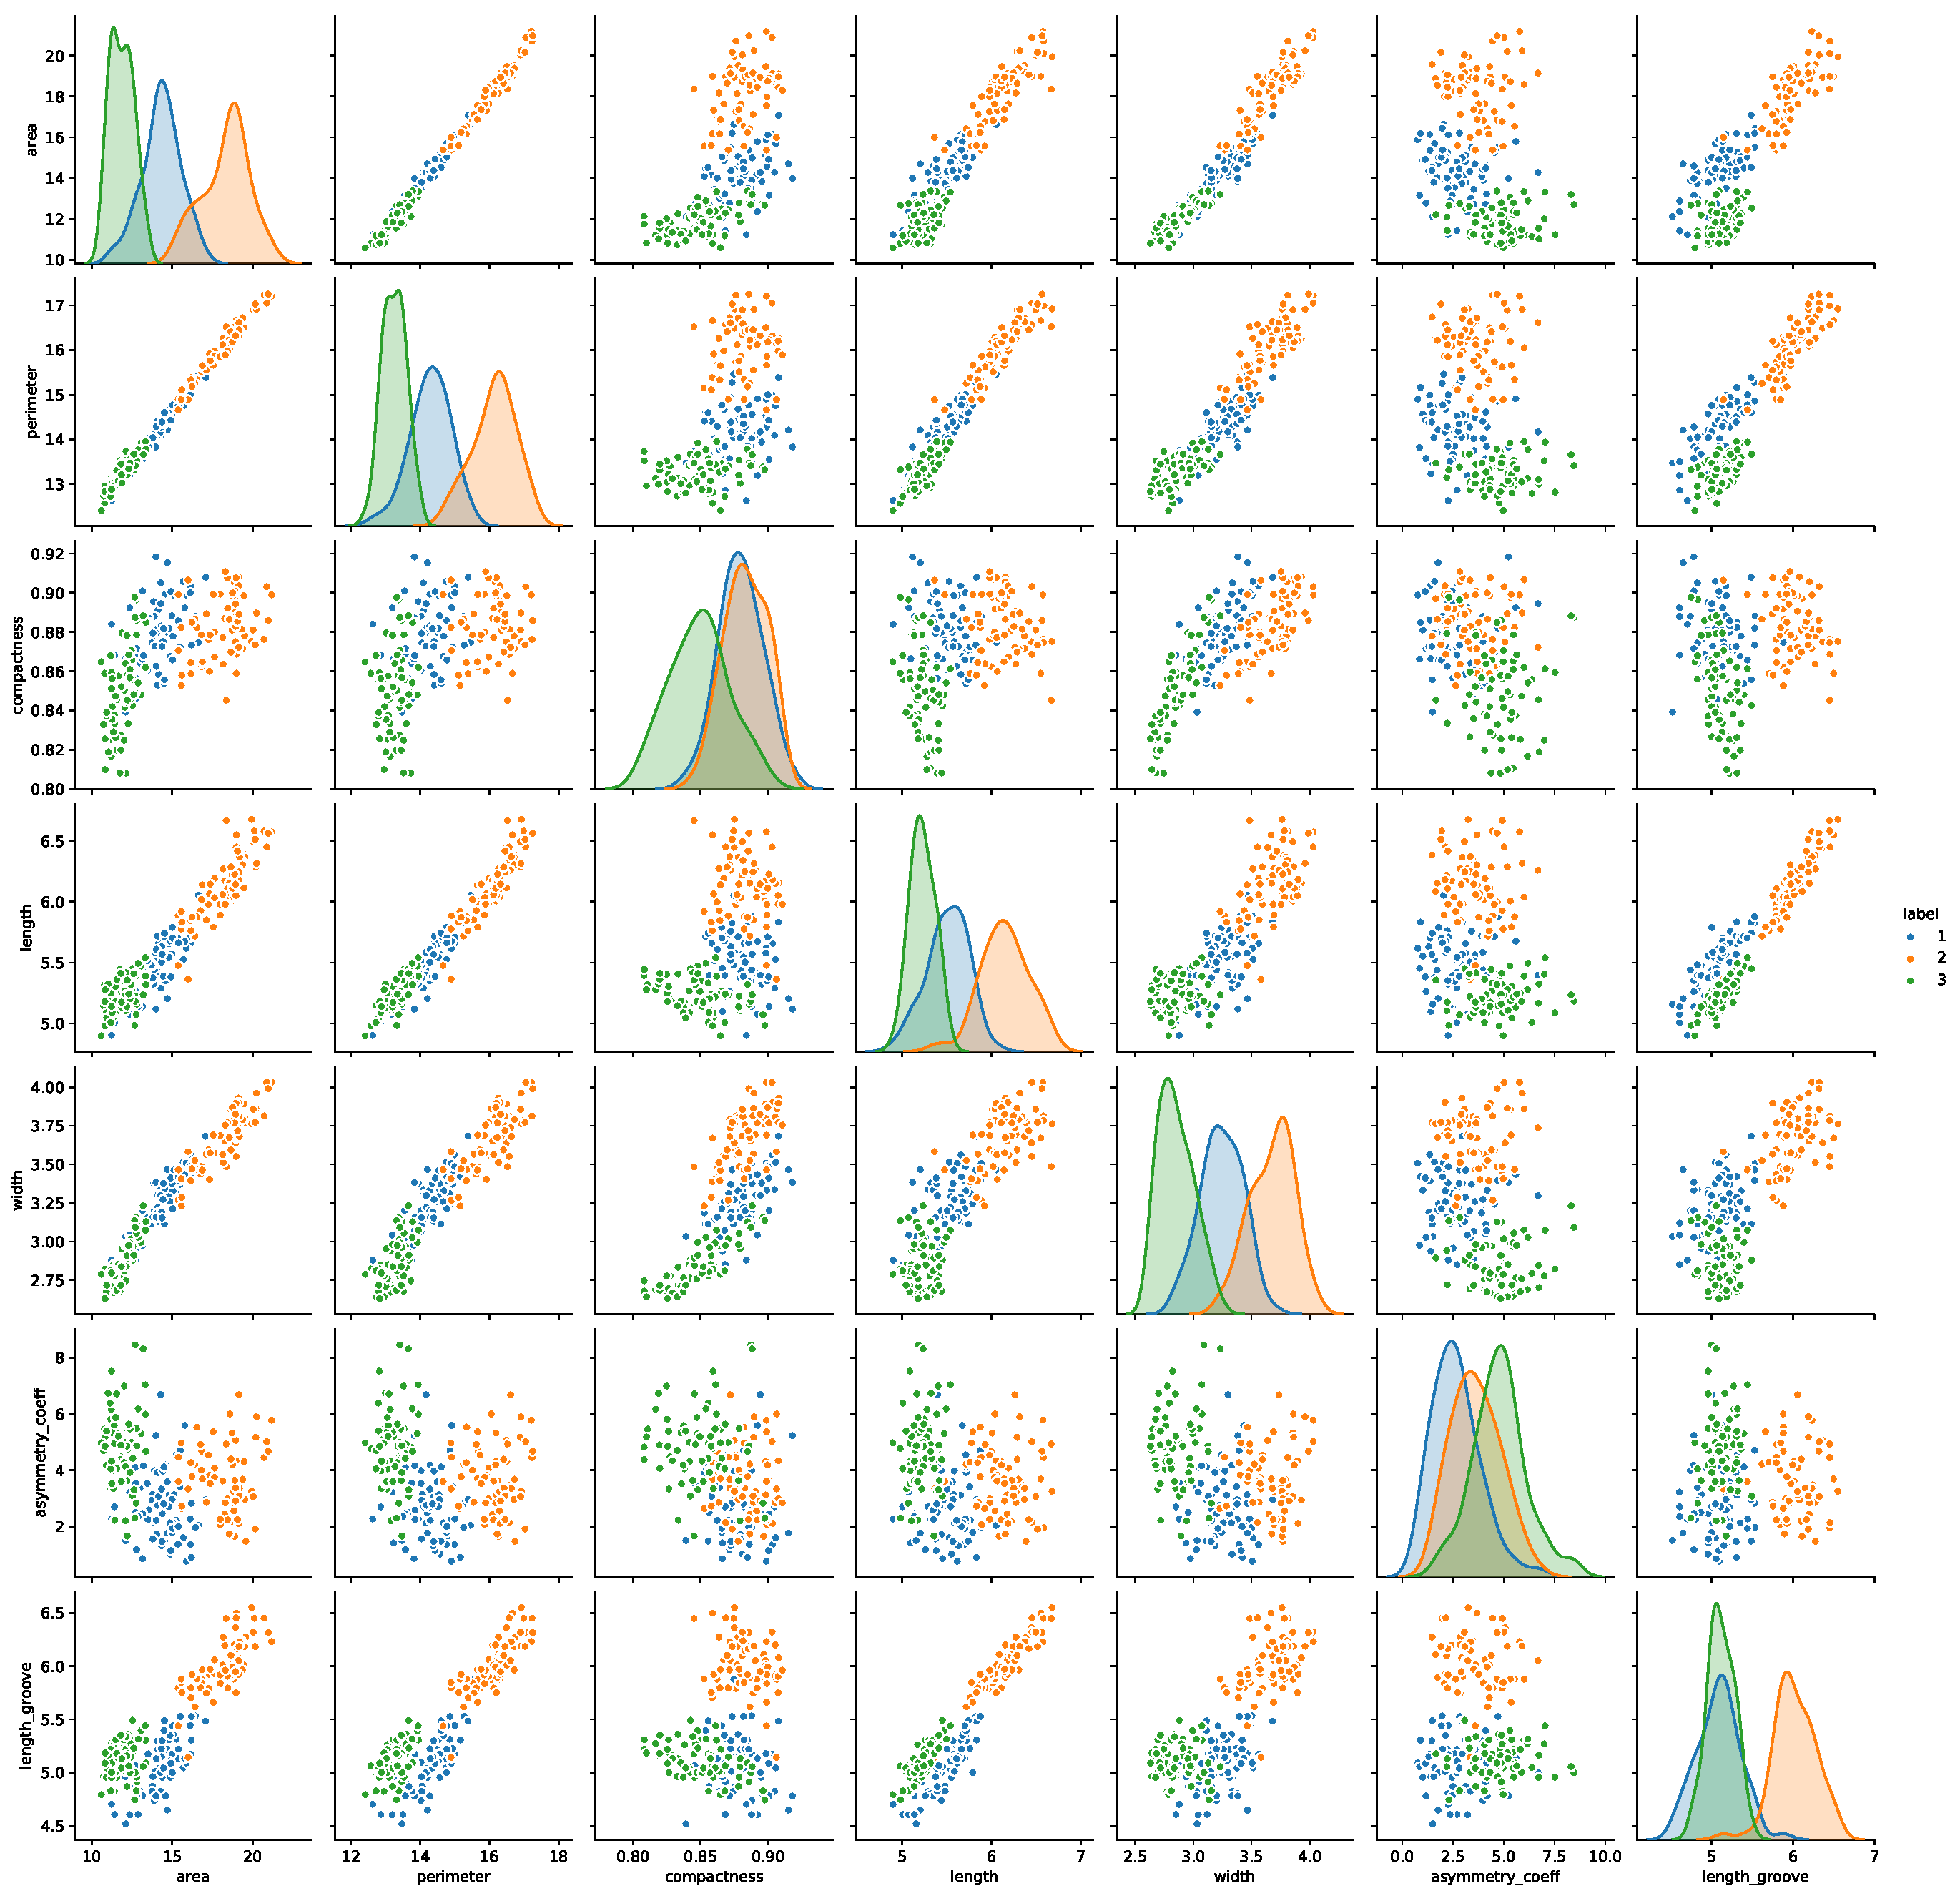
\includegraphics[width=0.75\textwidth]{images/seeds_pairplot.pdf}
\end{center}
\label{img:seeds_pairplot}
\end{figure}

A few things can be noted here: compactness is linearly dependent on two other features in the data set, calling into question what value this information can bring to a clustering method. Furthermore the area is not computed from other measurements, but is highly correlated with width and length and the perimeter. These relationships among others can be seen in figure \ref{img:seeds_pairplot}. Note that these plots have been colored according to their labels. Density plots on the diagonal already show distinct characteristics for the different varieties of kernels for certain features. For the clustering step of course the labels are removed from the data (this data set was included despite not being the typical application of clustering because it can serve as a sort of "control" for the clustering methods when looking at evaluation and conclusions).




\subsection{Red Wine Quality}
\textit{written by M.A.}\\

The data set was used as a wine quality data set and was gathered by Cortez et al. in 2009. It consists of labelled data and contains 11 attributes and 1599 instances. Its goal is to model wine quality based on physicochemical tests \cite{cortez2009modeling}. Due to privacy reasons, only physicochemical (inputs) and sensory (the output - quality) variables are available. That means there is no data about grape types, wine brand, wine selling price, etc..\newline

The input variables are: 
\begin{multicols}{2}
\begin{itemize}
    \item \textit {fixed acidity},
    \item \textit {volatile acidity}, 
    \item \textit {citric acid}, 
    \item \textit {residual sugar},
    \item \textit {chlorides}, 
    \item \textit {free sulfur dioxide}, 
    \item \textit {total sulfur dioxide},
    \item \textit {density}, 
    \item \textit {pH},
    \item \textit {sulphates} and 
    \item \textit {alcohol},
\end{itemize} 
\end{multicols}

which consist of floats and integer values.   \newline

While the \textit {fixed acidity} describes the acids in wine, which are mostly fixed or nonvolatile, the \textit {volatile acidity} describes the amount of acetic acid in wine, which can lead to an unpleasant vinegar taste, when it is too high.  The \textit {citric acid} is found in small quantities and can add freshness and flavor to wines. Its values lie between 0-1. \newline
Additionally, the attribute \textit{residual sugar} comprises the amount of sugar remaining after fermentation stops. It is rare to find wines with less than 1 gram/liter that is why even 15.5 gram/liter is being reached. \newline
\textit {Chlorides} describe the amount of salt in the wine, which is very less, specifically between 0.01 – 0.61. \newline
\textit {Free sulfur dioxides} and \textit {total sulfur dioxides} describe the amount of free and bound forms of SO2. In low concentrations, SO2 is mostly undetectable in wine, but at free SO2 its much easier.
Furthermore, \textit {density} of water is being used to describe wine quality and its values are between 
0.99 and 1. \newline
Additionally, the \textit {pH} value describes how acid or basic a wine is on a scale from 0 (very acid) to 14 (very basic). Most vines are between 3-4. \textit {Sulphates} describe a wine additive.
The last attribute \textit {alcohol} holds details about the percent alcohol content of the wine. 
\textit {Quality} is described as an output variable, which is based on the sensory data. The score is between 0 and 10 \cite{kaggle-redwine}.\newline
This dataset does not include empty columns, nor does it have empty values.
Figure \ref{fig:wine_stats} depicts the spread of each attribute in the pillar chart of the wine quality data set \cite{kaggle-redwine}. This data set is suggested to be used for regression or classification modelling \cite{kaggle-redwine}.
That’s why we have chosen it for clustering. \newline

\begin{figure}[H]
%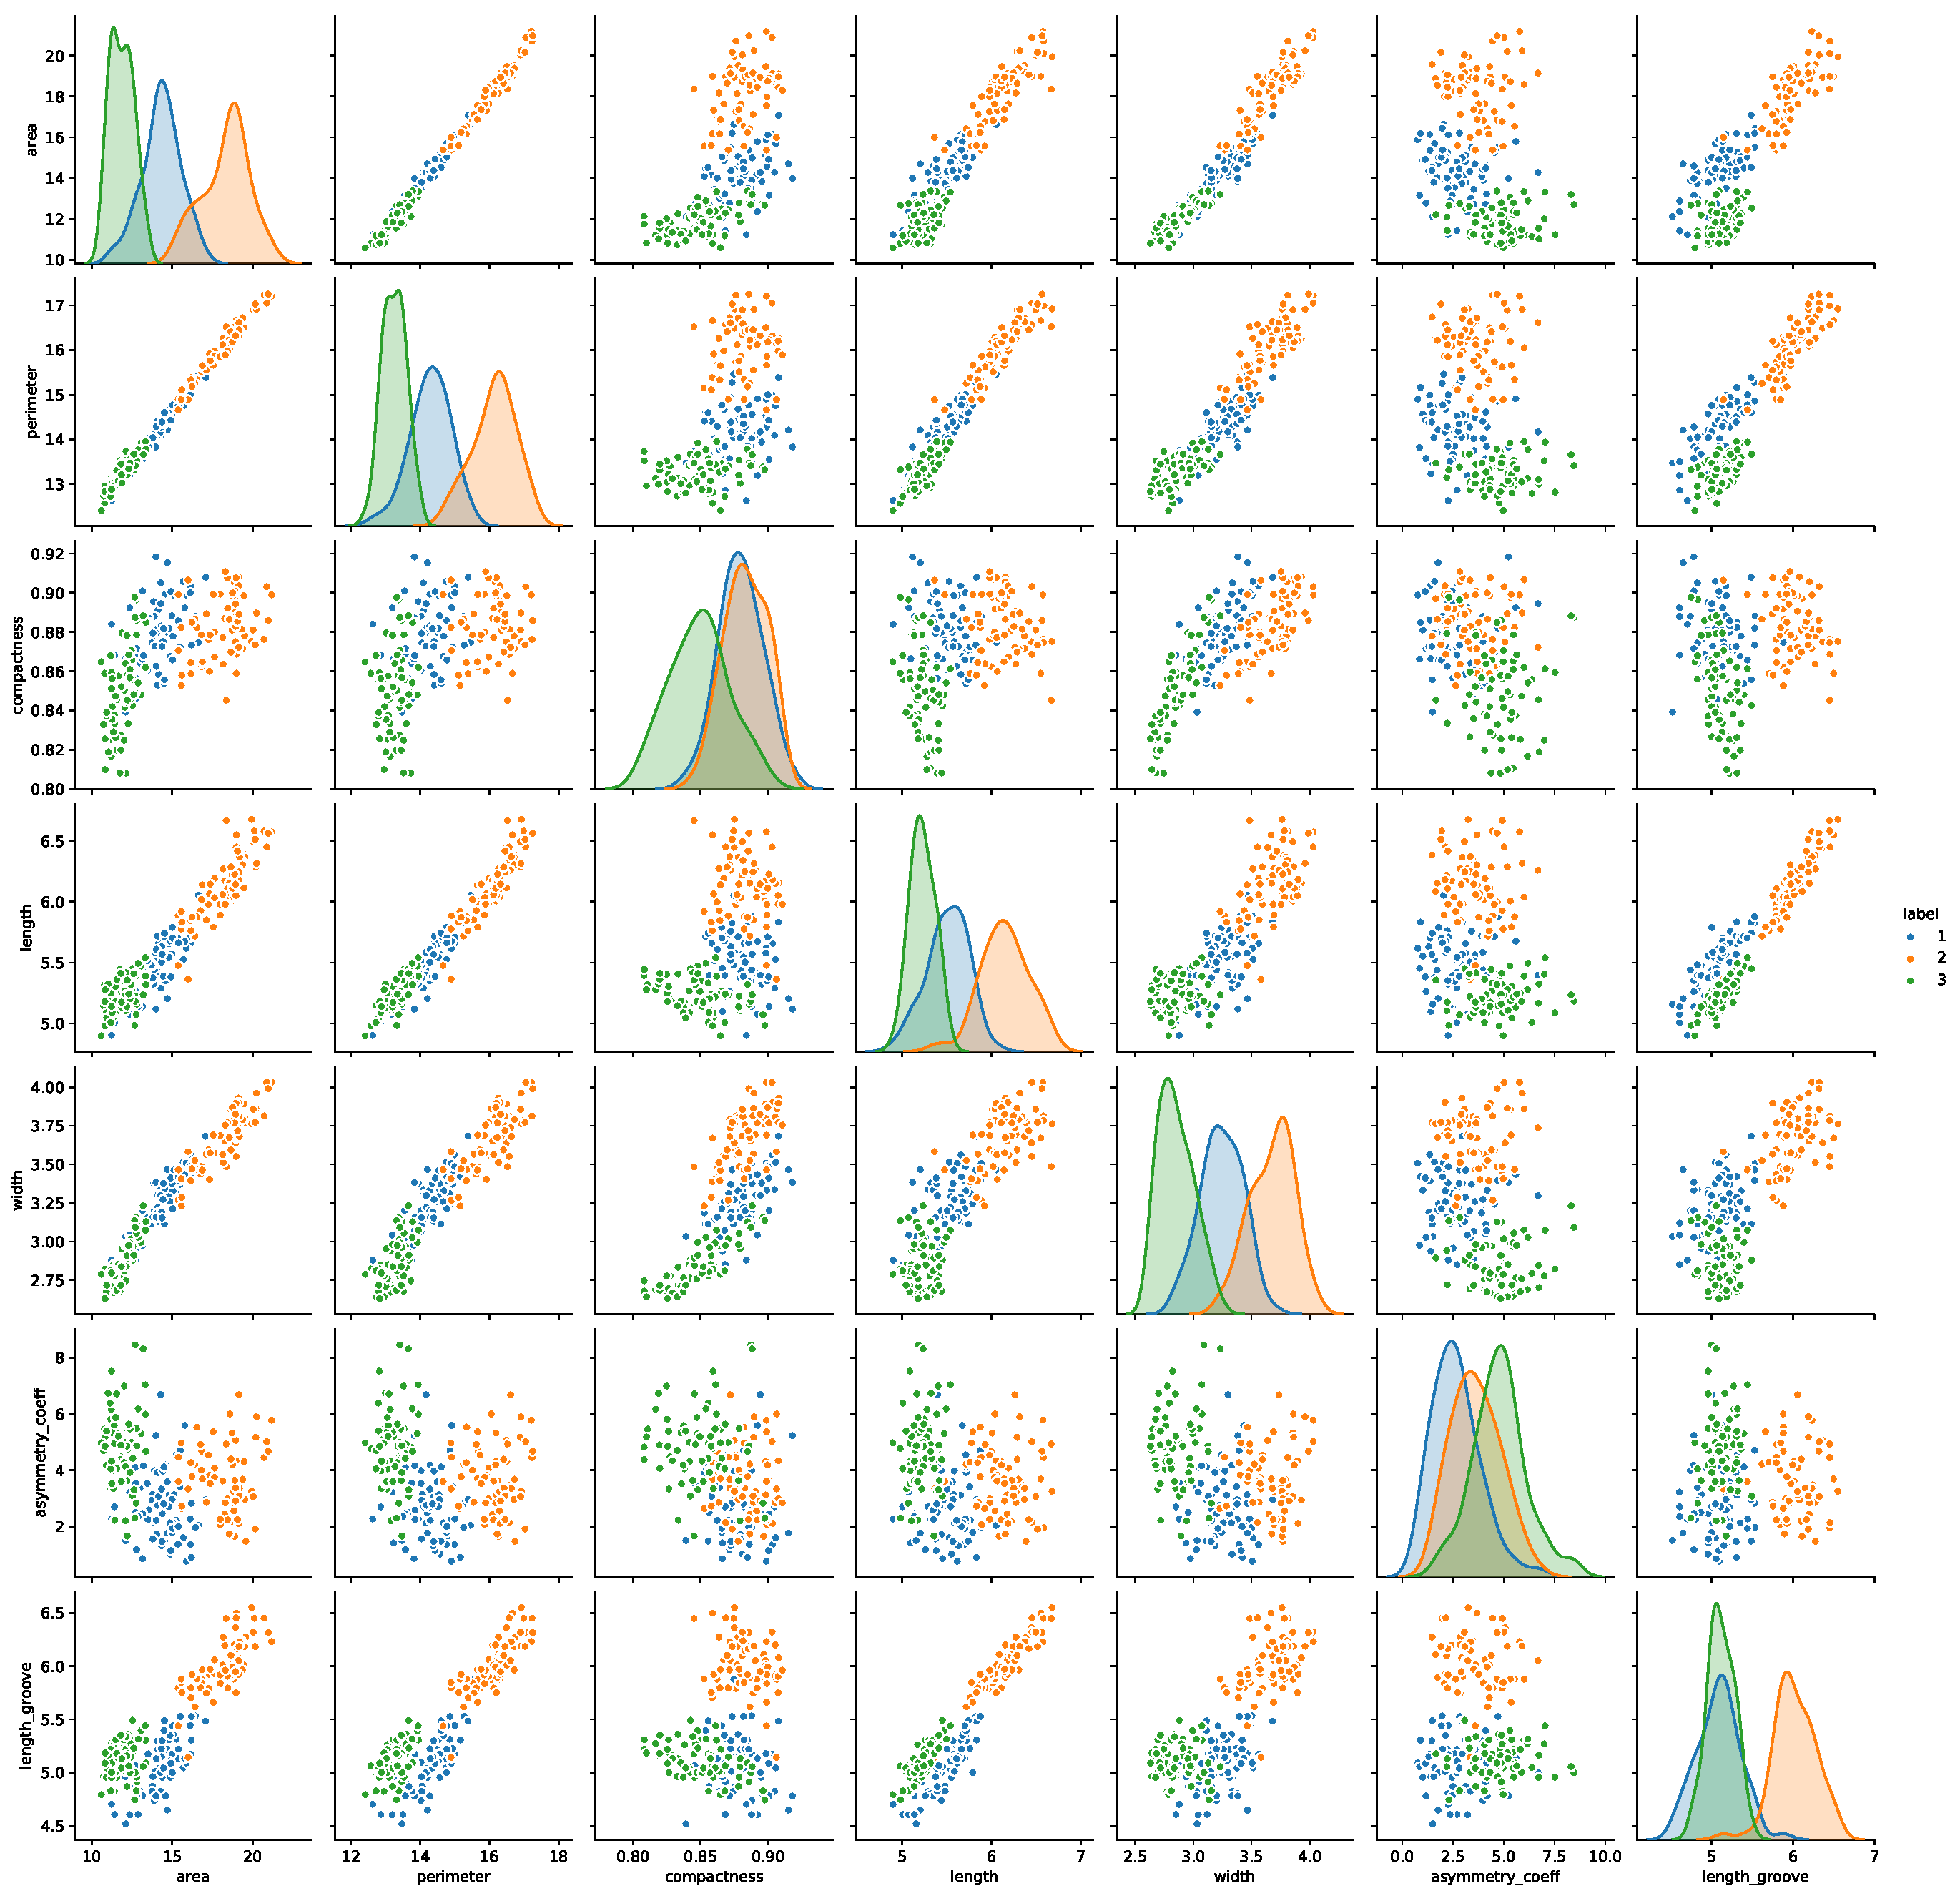
\includepdf[pages=-,scale=.4]{images/seeds_pairplot.pdf}
\centering
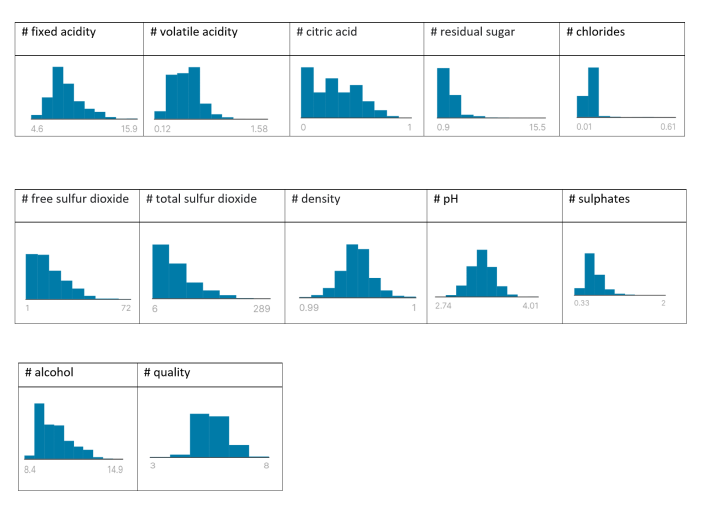
\includegraphics[width=1\textwidth]{images/wine_table.png}
\caption{Spread of each attribute of the wine quality data set}
\label{fig:wine_stats}
\end{figure}

\section{Description of Evaluation Module}
\label{sec:evaluation_description}
Due to the nature of clustering as an unsupervised machine learning method, it is typically applied to datasets lacking prior information on grouping. Therefore measuring the performance of each method can only be performed on the data and the labeling produced by each clustering algorithm. These types of calculations are commonly called \textit{internal cluster validation} indices.

Differentiating by the way compactness and separation are measured \cite{balbi2016cosine} split indices into two groups. There are graph based indices: C Index, Dunn, Gamma, G+, McClain-Rao, Point Biserial, Silhouette, Tau, and there are prototype based indices: Calinski-Harabasz, Davies-Bouldin, Pakhira-Bandyopadhyay-Maulik (PBM), Ratkowski-Lance, Ray-Turi, Xie-Beni, Wemmert-Gancarski. 

We have decided to use two indices from each group: \gls{DI} and \gls{SI}, \gls{CH}, \gls{DB}. 


\subsection{Dunn Index}
\textit{written by M.A.}\\

% Dunn \cite{dunn1974well} brief explanation and reasons.

The Dunn Index (in short DI) is a metric for evaluating clustering algorithms. Its aim is to identify sets of clusters \cite{dunn2016rizzo}. It is used for measuring an internal validation of clustering results \cite{BENNCIR2021102751}. \newline

For each cluster, compute the distance between each of the objects in the cluster and the objects in the other clusters. Use the minimum of this pairwise distance as the inter-cluster separation (min. separation). For each cluster, compute the distance between the objects in the same cluster. Use the maximal intra-cluster distance (i.e maximum diameter) as the intra-cluster compactness. Calculate the Dunn index (D) as follow: \newline

D = $\frac{min.separation}{max.diameter}$ \cite{BENNCIR2021102751} \newline

The higher the value of the resulting Dunn index, the better the clustering
result is considered, since higher values indicate that clusters are Compact.
That means the greater the better \cite{dunnblog2019rizzo}. \newline

\subsection{Calinski-Harabasz Index}
\textit{written by B.L.}\\

The Calinski-Harabasz criterion \cite{calinski1974dendrite} is defined as a poportional measure of within cluster variance to between cluster variance. That is why it is also known as the \gls{VRC}. Mathematically this means
\begin{equation}
        CH = \frac{S_{B}}{S_{W}}\frac{m-K}{K-1} = \frac{\sum_{k=1}^{K} \left | C_{k} \right | \left \| c_{k} - \sum_{x' \in X}^{} x' \right \|^{2}}{\sum_{k=1}^{K}\sum_{x \in C_{k}}^{} \left \| x - c_{i} \right \|^{2}} \frac{m-K}{K-1}
\end{equation}
utilizing the same notation as equation \ref{eq:kmeans_basic_other}. Between-cluster variance is divided by within-cluster variance. Dividing the data into more partitions of course reduces within-cluster variance, which is why there is also a scaling factor (second fraction representing degrees of freedom) to account for it. In comparison to \gls{DB} between-cluster variance is calculated in relation to the center of the data set in place of between individual cluster centers themselves. 

Due to its construction (distance measure) this index performs well when clusters form mostly convex shapes. This can lead to mis-evaluation if the underlying data does not comprise of such globular clusters so a method capturing this might score lower while actually fitting the data better. It may therefore be better suited to compare different parameters for the same algorithm instead of comparing different algorithms. A comparative study of 30 cluster validation indices \cite{arbelaitz2013extensive} ranks \gls{CH} performance in evaluating fit near the top in many applications, particularly when evaluating K-Means results as expected.
    
\subsection{Davies-Bouldin Index}
\textit{written by J.M.}\\

%Davies-Bouldin \cite{davies1979cluster} brief explanation and reasons.
The Davies-Bouldin index is a metric to evaluate clustering algorithms and it was developed by David Davies and Donald Bouldin in 1979 \cite{davies1979cluster}. 
It is used to check the validity of the clusters. To reach this, the Davies-Bouldin Index tries to maximize the intern-cluster distance 
and on the other side tries to minimize the intern cluster distance. 
The Davies-Bouldin index is defined as 
	
$ \bar{R} \equiv \frac{1}{N} \sum_{i=1}^{N} R_i  $ \\
where N is the number of cluster and $R_i$ is the maximum of $R_{ij}$ where i$\neq$j \\
	
$R_{ij} \equiv \frac{S_i+ S_j}{M_{ij}}$ \\
where $M_{ij}$ is the Minkowski metric which can be descibed as: \\ $M_{ij} = \{ \sum_{k=1}^{N} |a_{ki} - a_{kj}  |^p    \} ^{  \frac{1}{p}}   $ 	
	
$S_{ij} = \{\frac{1}{T_i} \sum_{j=1}^{T_i} |X_{j} - A_{i}  |^q    \}^\frac{1}{q}$ \\
	
If q =1 	$S_{ij}$ is the Euclidean distance between centroids.  \\
  
For our evaluation we use the implementation from sklearn of this metric. This metrics calculate a score. Zero is the lowest score that can be reached. If a score is closer to zero, it related that there is a better seperation between the calculated clusters. 

\subsection{Silhouette Score}
\label{Silhouette Score}
\textit{written by L.B.}\\

Cluster validation indexes are used to assess clustering quality. That means it is investigated whether the resulting clusters reflect natural structures in the data or whether clusters rather determine artificial groups. In general, the ratio of dissimilarity between data points within the same cluster to dissimilarity between data points in different clusters is a measurement for clustering quality. 
The Silhouette Score is one of such cluster validation indexes which can be applied to evaluate clustering results if Euclidean distance measures can be calculated on the underlying dataset. According to that, a clustering result as well as proximity scores between all data points have to be provided to be able to apply the Silhouette Score. 
For a single data point, distances to all the data points assigned to the same cluster are calculated. Here, the mean of all these distances is called \textit{a}. After that, the nearest cluster for each data point has to be found. This can be done by iteratively calculating the mean of distances between the single data point and all data points within another cluster until distances for all clusters have been computed. The minimum average distance determines the nearest cluster for the single data point. 
The minimum average distance is called \textit{b} here. The Silhouette Score for data point i is calculated using the following formula:
\begin{align*}
	s(i)=\frac{b - a}{max(a, b)}
\end{align*}
The mean of all the Silhouette Scores for each individual data point determines the Silhouette Score for the whole dataset. As the nearest cluster has to be found for each of the included data points, the Silhouette Score can only be computed as soon as more than one cluster exists \cite{rousseeuw1987silhouettes}.
Taking a closer look at extreme cluster results determines how to interpret the Silhouette Score values. Given a partition where the mean intra-cluster distance \textit{a} is extremely low while the mean inter-cluster distance \textit{b} is high, the Silhouette Score would tend to be \mintinline[bgcolor=code-bg]{python}{1}. Hence, a Silhouette Score of \mintinline[bgcolor=code-bg]{python}{1} corresponds to a well-partitioned dataset because the mean of distances between single points and other clusters than the one it is assigned to is large. Analogously, a value of \mintinline[bgcolor=code-bg]{python}{-1} corresponds to a partition where the inter-cluster distance \textit{b} is much larger than the intra-cluster distance \textit{a}. Thus, the data points are not assigned to their nearest clusters, resulting in a misclassification. If the Silhouette Score is equal to zero, means of inter- and intra-cluster distances are close to each other and it is unclear which cluster the point should be assigned to. In this case, the partition can also contain overlapping clusters \cite{rousseeuw1987silhouettes}.
For the calculations of Silhouette Scores, we make use of the implementation provided from sklearn \cite{sklearn_api}.
We make use of the Silhouette Score as it can be applied on cluster results generated with any clustering technique. It therefore provides an intuitive way of comparing the results of different algorithms to each other. One disadvantage is that Silhouette Scores are higher for convex clusters. As some density-based clustering algorithms like Mean Shift explicitly allow the creation of non-convex clusters, the obtained Silhouette Scores could possibly be lower than results created applying other clustering techniques. This is further investigated in the evaluation part. 
%\item Gap \cite{tibshirani2001estimating} brief explanation and reasons.

\subsection{Results}

In the following there is a discussion of the results of all clustering efforts in detail. A brief overview of the evaluation results can be found in table \ref{tab:evalutaion_table}. For each data set there is a row for each algorithm used. In columns are the results for each index. The cells represent the highest (lowest for \gls{DB} respectively) value achieved by applying various parameter configurations. It should be noted that comparing results across different methods does not show the entire picture but it can yield indications on performance. MORE WHEN RESULTS.

\begin{table}[H]
\begin{center}
%\resizebox{\textwidth}{!}{%
\begin{tabular}{lrrrr}
Data and Method & \multicolumn{1}{c}{\gls{CH}} & \multicolumn{1}{c}{\gls{DB}} & \multicolumn{1}{c}{\gls{SI}} & \multicolumn{1}{c}{\gls{DI}} \\ \hline
 &  &  &  &  \\
\textbf{Housing} &  &  &  & \\
K-Means & 1621.90 & 1.014 & 0.721 & 0.525 \\
Mean Shift & 1.567 & 2.346 & 3.457 & 4.856 \\
Affinity & 1.567 & 2.346 & 3.457 & 4.856 \\
Spectral & 1.567 & 2.346 & 3.457 & 4.856 \\
 &  &  &  &  \\
\textbf{Mall} &  &  &  &  \\
K-Means & 301.02 & 0.901 & 0.479 & 0.843 \\
Mean Shift & 1.567 & 2.346 & 3.457 & 4.856 \\
Affinity & 1.567 & 2.346 & 3.457 & 4.856 \\
Spectral & 1.567 & 2.346 & 3.457 & 4.856 \\
 &  &  &  &  \\
\textbf{Seeds} &  &  &  &  \\
K-Means & 369.55 & 0.979 & 0.492 & 0.091 \\
Mean Shift & 1.567 & 2.346 & 3.457 & 4.856 \\
Affinity & 1.567 & 2.346 & 3.457 & 4.856 \\
Spectral & 1.567 & 2.346 & 3.457 & 4.856 \\
 &  &  &  &  \\
\textbf{Wine} &  &  &  &  \\
K-Means & 3116.82 & 0.901 & 0.603 & 0.049 \\
Mean Shift & 1.567 & 2.346 & 3.457 & 4.856 \\
Affinity & 1.567 & 2.346 & 3.457 & 4.856 \\
Spectral & 1.567 & 2.346 & 3.457 & 4.856
\end{tabular}%
%}
\end{center}
\caption{Comparing All Algorithms On All Data Sets For All Evaluation Indices}
\label{tab:evalutaion_table}
\end{table}


\subsubsection{Seeds K-Means}
\textit{written by B.L.}\\

\vspace{-0.5cm}
\begin{table}[H]
\begin{center}
%\resizebox{\textwidth}{!}{%
\begin{tabular}{crrrr}
$K$ & \multicolumn{1}{c}{\gls{CH}} & \multicolumn{1}{c}{\gls{DB}} & \multicolumn{1}{c}{\gls{SI}} & \multicolumn{1}{c}{\gls{DI}} \\ \hline
2 & 351.235 & 0.688 & 0.519 & 0.038 \\
3 & 375.804 & 0.753 & 0.471 & 0.085 \\
4 & 327.439 & 0.825 & 0.412 & 0.020 \\
5 & 310.331 & 0.915 & 0.361 & 0.091 \\
6 & 302.344 & 0.917 & 0.366 & 0.106 \\
7 & 294.385 & 0.939 & 0.350 & 0.077 \\
8 & 297.502 & 0.937 & 0.362 & 0.083 \\
\end{tabular}%
%}
\end{center}
\caption{K-Means Seeds Dataset Indices by Number of Clusters}
\label{tab:kmeans_seeds_table}
\end{table}

Table \ref{tab:kmeans_seeds_table} contains the index scores for each of the indices selected as columns and the number of clusters as rows. An easier representation of this data is a line chart which can be seen in figure \ref{fig:kmeans_seeds_comparison_plot} and in the following description of results. More than simply a tool to compare scores between methods, these can help in identifying the number of clusters (or other parameters below) best fit to represent the data. So what can be learned from the data: If there is a clear maximum value for an index it indicates looking at that value to gain insight on the fit. If there is no clear maximum value, one can try to employ the so called elbow criterion (see section \ref{subsec:method_kmeans}) where a distinct change in direction for a graph might indicate a value worth examining. If there is neither there seems to be no information gain at hand from that particular index for this application.

\begin{figure}[H]
\caption{K-Means Seeds Dataset Indices by Number of Clusters}
\begin{center}
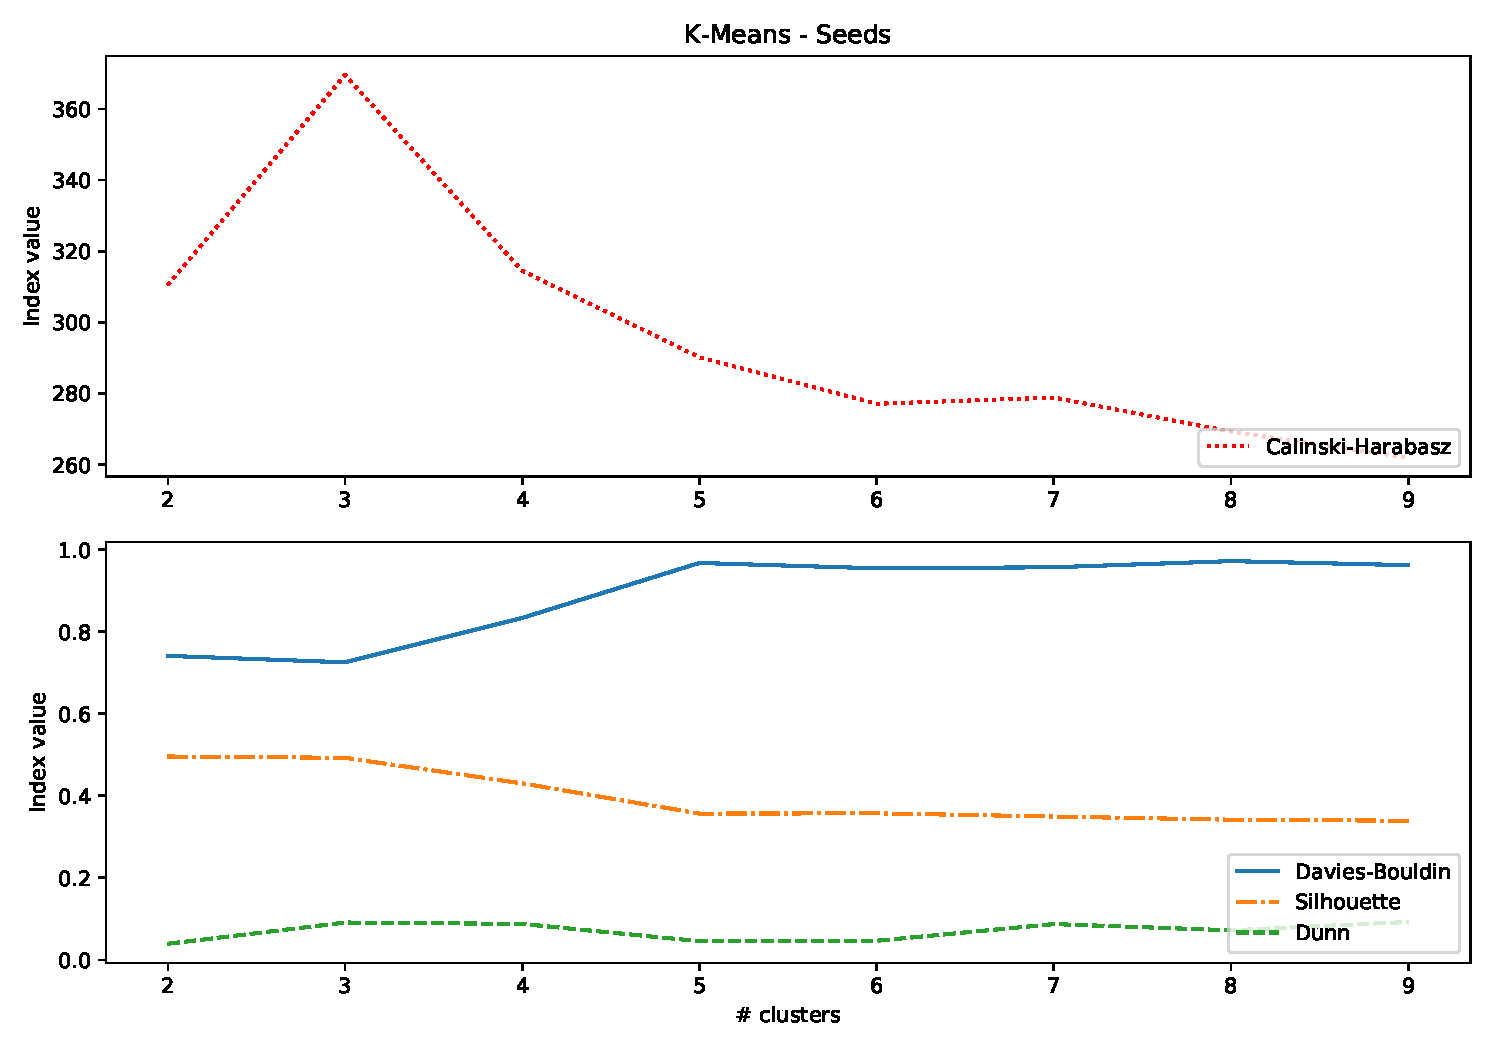
\includegraphics[width=1.0\textwidth]{images/kmeans_seeds_index_plot.pdf}
\end{center}
\label{fig:kmeans_seeds_comparison_plot}
\end{figure}

\vspace{-0.5cm}
Looking at figure \ref{fig:kmeans_seeds_comparison_plot} (one line for each index, two panels because of the vastly different scale of \gls{CH}) one can see a clear maximum in \gls{CH} value and a local maximum in \gls{DI} as well as a change in slope for \gls{SI} at three clusters each. Following the described logic, \gls{DB} suggests also considering five clusters as an option. 

As mentioned in section \ref{sec:data_description} this dataset originally comes with labels which allows to use them as a benchmark to see how the clustering performs. Plotting (figure \ref{fig:kmeans_seeds_tsne}) two dimensional representations (see t-SNE in section \ref{sec:frontend_description}) of the K-Means clustered result and the original data shows a few things: the algorithm has, as expected, produced non-overlapping mostly contiguously shaped clusters in contrast to the original data. However using three clusters has generally produced a reasonably good fit, as is supported by an accuracy of 89.5\%, precision of 90\% and recall of 89.5\% to name a few standard metrics.

\begin{figure}[H]
\caption{Seeds Data Set Comparison Clustering and Original Labels}
\begin{center}
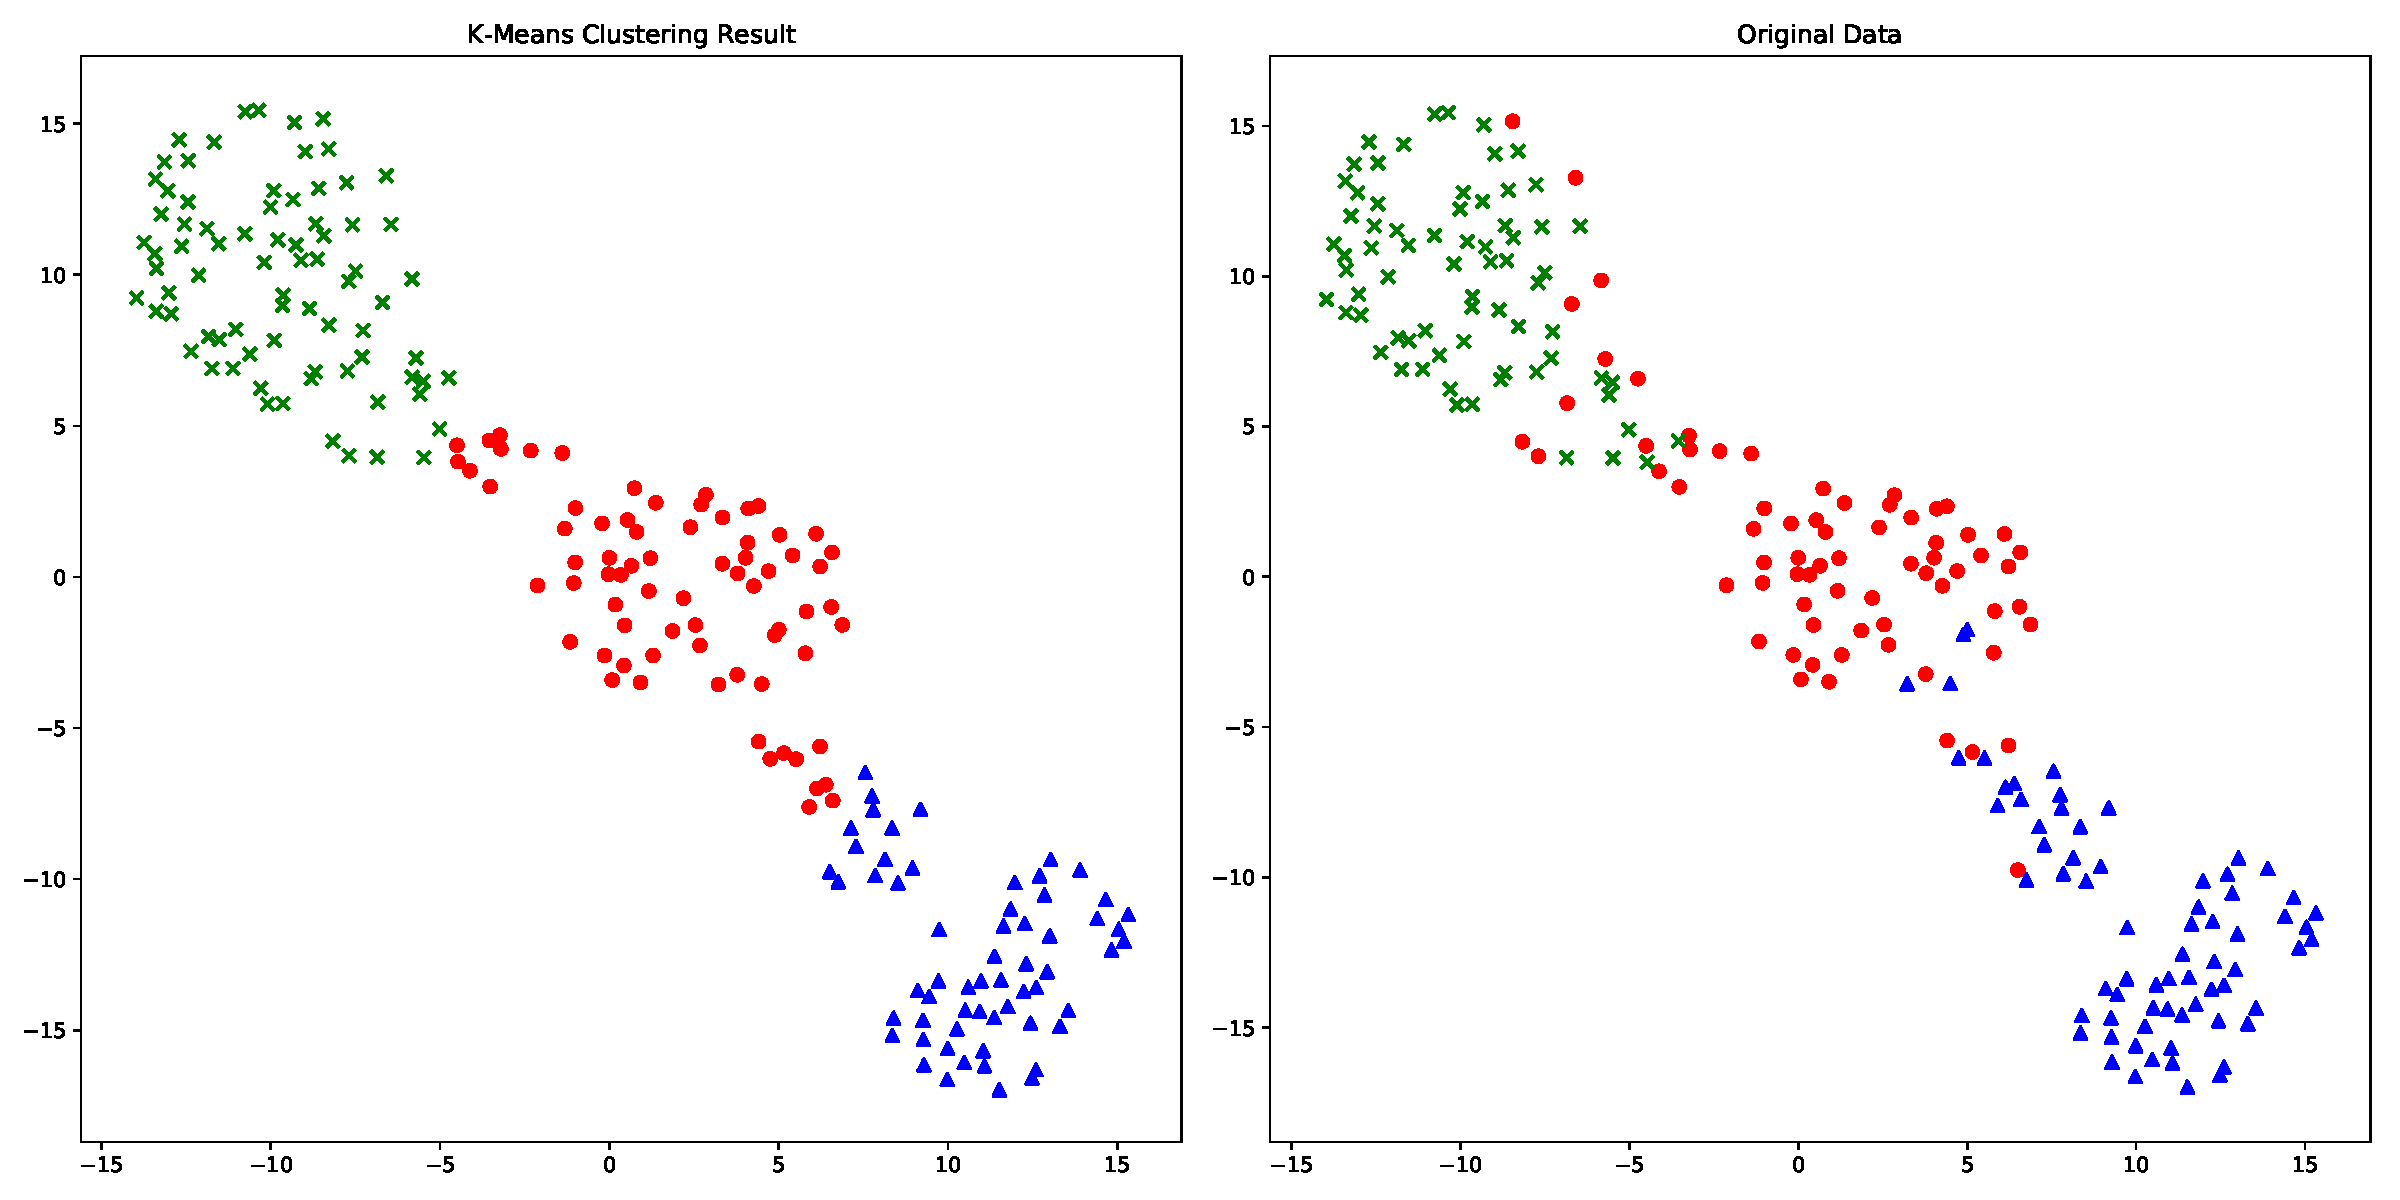
\includegraphics[width=1.0\textwidth]{images/kmeans_seeds_tsne.pdf}
\end{center}
\label{fig:kmeans_seeds_tsne}
\end{figure}

%continuous data in all features makes application straight forward
%as shown in table \ref{tab:k-means_seeds_table} data on how many clusters to choose not clear
%looking at chart in \ref{fig:kmeans_seeds_indices_plot} makes comparison easier. shows \gls{CH} with significant signal at three clusters and \gls{DI} flattening out after three clusters while \gls{SI} falling after three clusters. only \gls{DB} highest at seven clusters. in light of this analysis it doesn't seem unreasonable to select three clusters as the best fit. looking at the data in 3d, see figure

\subsubsection{Mall Customers K-Means}
\textit{written by B.L.}\\

As one of the features is categorical (gender), this is not an ideal application of the K-Means clustering method. The categories can be resolved into discrete values so that calculations can be run, but the arbitrary nature of this does not really allow for good interpretation of the results. An exemplary three dimensional plot \ref{fig:kmeans_customers_3d} shows the issue: 

\begin{wrapfigure}{r}{0.5\textwidth}
  \centering
    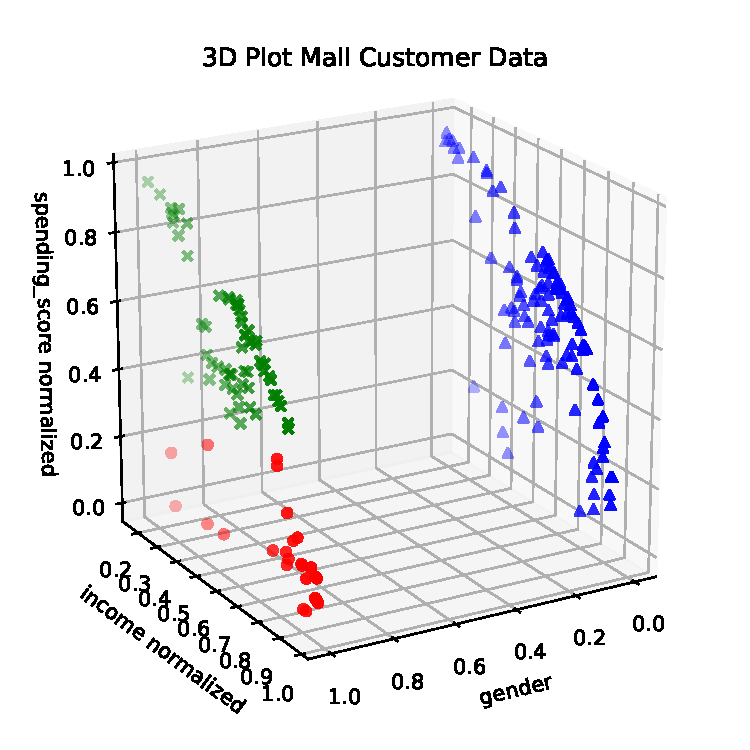
\includegraphics[width=0.48\textwidth, clip]{images/kmeans_customers_3d.pdf}
  \label{fig:kmeans_customers_3d}
  \caption{Split Data Due To {Categorical} Feature}
\end{wrapfigure}

gender is represented on the z-axis and the two manifestations simply rip the data into two partitions. When gender is encoded as 0 and 1, this showed almost no effect. When using 0 and 100, it leads to a doubling in the index-recommended number of clusters. One attempt to deal with this is to scale all data between 0 and 1 but this aggravated the problem instead of improving on it. Extensions of the K-Means method have been devised to deal with this type of data (as described in section \ref{subsec:method_kmeans}) but their application here seems beyond the scope of this work. Using the gender feature also does not improve scores in the evaluation methods used. Given these circumstances, considering plot \ref{fig:kmeans_customers_indices_plot} suggests considering the results for 2 (\gls{CH}, \gls{DB}, \gls{SI}), 7 (\gls{DB}) or 8 (\gls{CH}) clusters.

\begin{figure}[h]
\caption{K-Means Mall Customers Dataset Indices by Number of Clusters}
\begin{center}
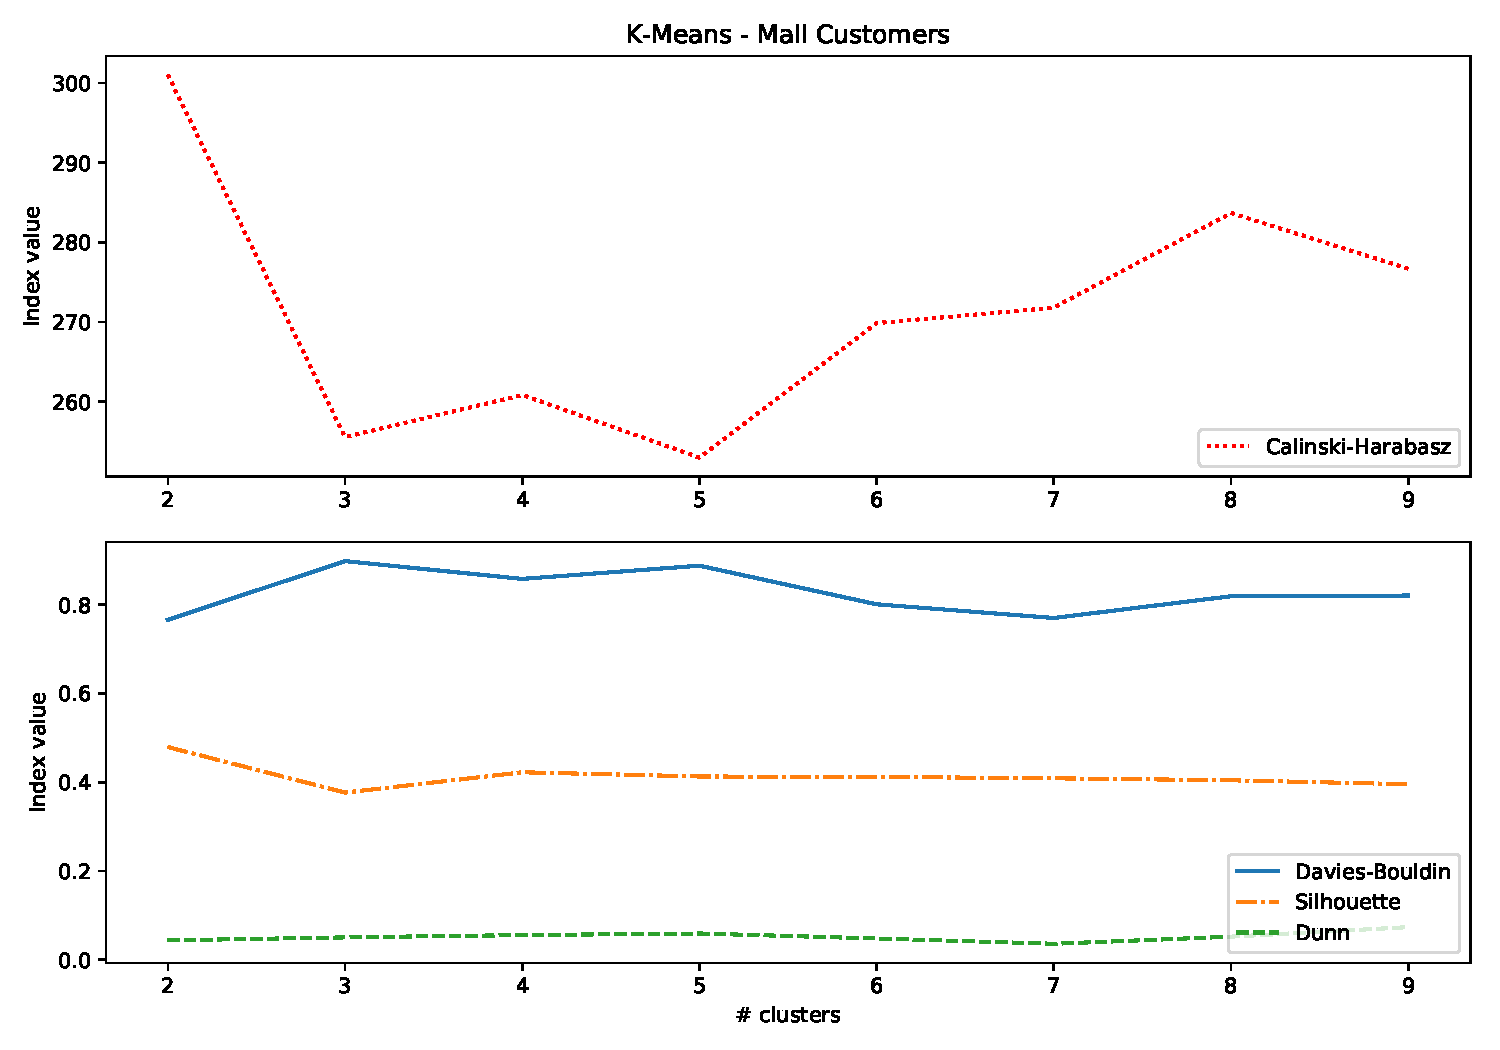
\includegraphics[width=1.0\textwidth]{images/kmeans_customers_index_plot.pdf}
\end{center}
\label{fig:kmeans_customers_indices_plot}
\end{figure}

\vspace{-0.5cm}
The dataset contains four features, three of which have a measurable and interpretable impact on clustering, which lends itself to a visual comparison in three dimensional space. Figure \ref{fig:kmeans_customers_3d_multi} shows three plots, one for each suggested number of clusters. The highest overall evaluation scores were achieved for two clusters and purely from a visual standpoint this seems to hold up.

\begin{figure}[h]
\caption{Mall Customers 3D Plot Clustering Options}
\begin{center}
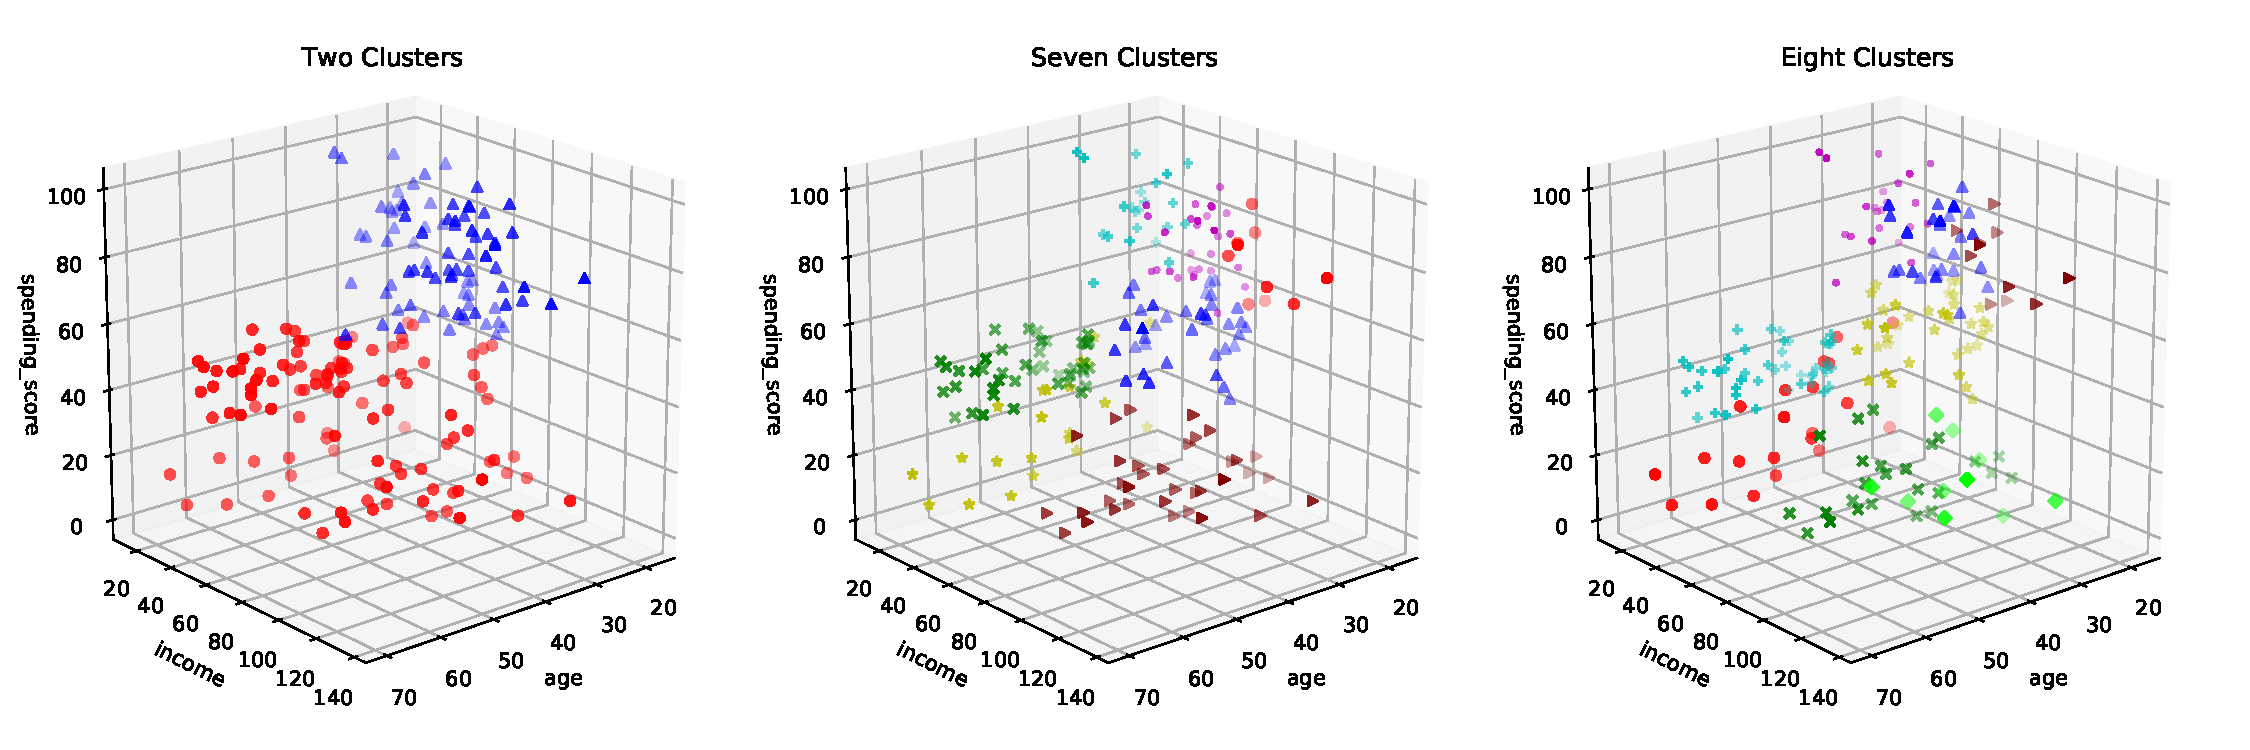
\includegraphics[width=1.0\textwidth]{images/kmeans_mall_3d_multi.pdf}
\end{center}
\label{fig:kmeans_customers_3d_multi}
\end{figure}
\vspace{-0.5cm}

%Rotating the plot shows that both partitions contain very similar clusters but due to the way K-Means works they are not recognized as the same. The data shows either two clusters (simply male cluster and female cluster) or an ideal number of clusters double the amount perceived by a human to be reasonable.

\subsubsection{Housing K-Means}
\textit{written by B.L.}\\

This dataset is challenging for K-Means clustering due to the high number of features. As described in section \ref{subsec:method_kmeans} the concept of distance does not hold up well in high dimensional cases. Attempts to transform the data into lower dimensional representations through principle component analysis did not yield an improvement in clustering performance. Data in figure \ref{fig:kmeans_housing_indices_plot} suggests to consider 2 (\gls{DI}), 3 (\gls{SI}, \gls{DB}) or 4 (\gls{CH}) clusters.

\begin{figure}[H]
\caption{K-Means Housing Dataset Indices by Number of Clusters}
\begin{center}
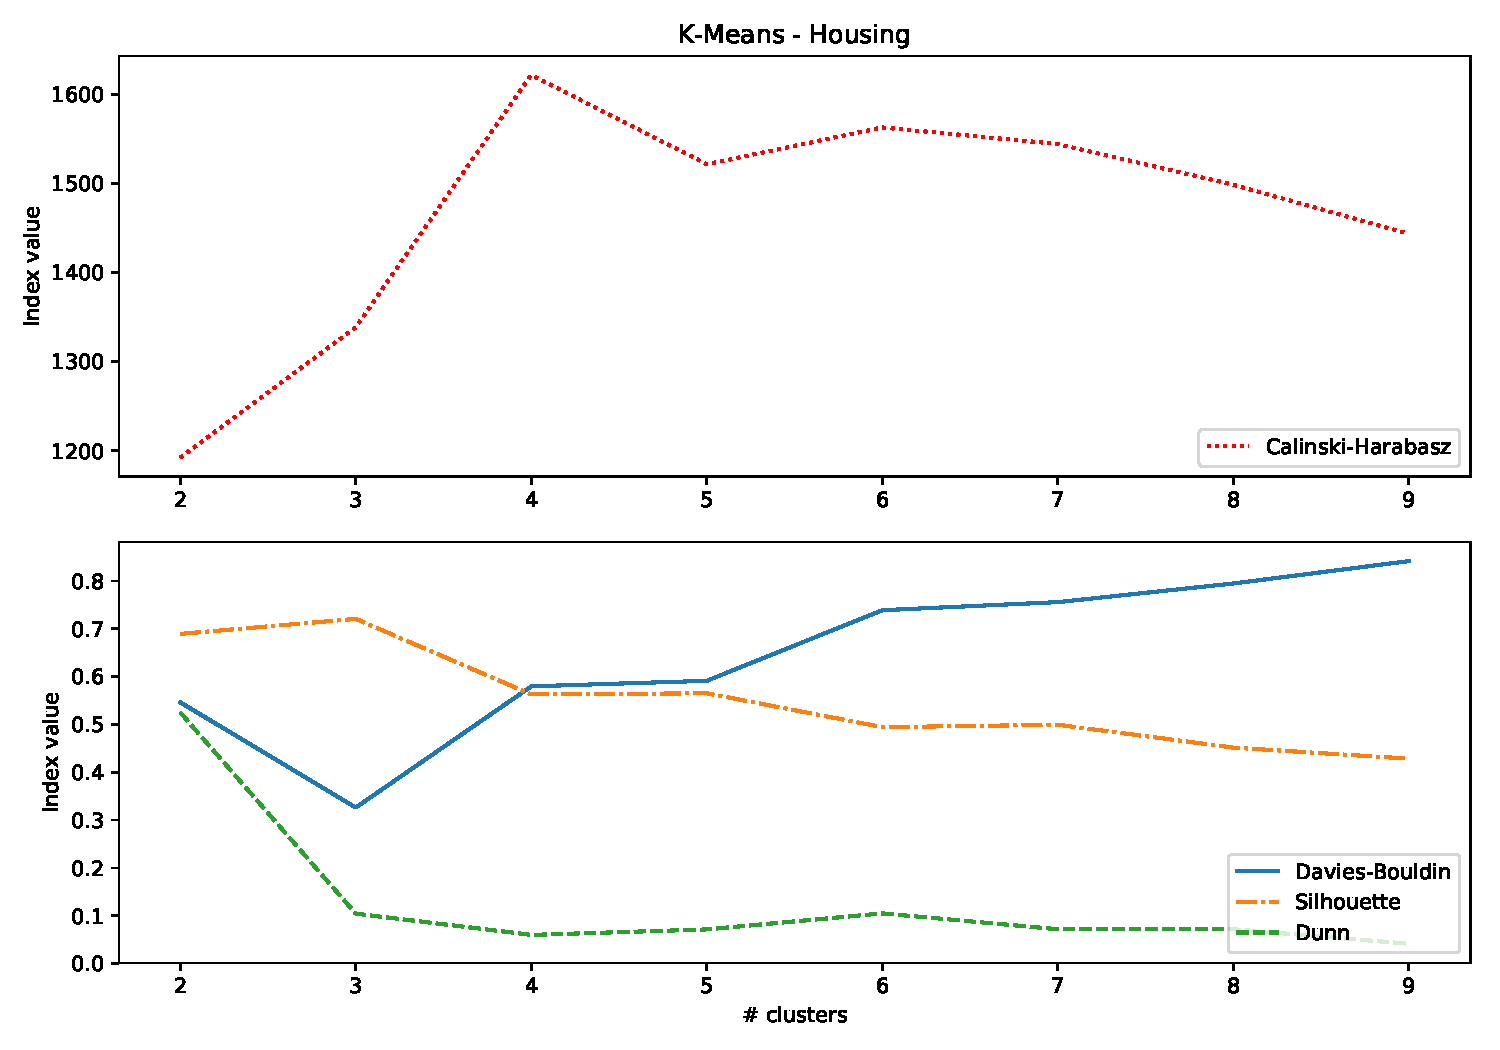
\includegraphics[width=1.0\textwidth]{images/kmeans_housing_index_plot.pdf}
\end{center}
\label{fig:kmeans_housing_indices_plot}
\end{figure}

\vspace{-0.5cm}
Due to the high dimensionality of the data, looking at different angles in three dimensions to get an understanding is not feasible. Therefore a two dimensional transformation (t-SNE, see section \ref{sec:frontend_description}) will help. Figure \ref{fig:kmeans_housing_2d_comparison} shows the case of two, three and 15 as representation for a significantly higher number of clusters. From a visual standpoint, two and three clusters seem to capture the visibly separation of parts of the data quite well, while the high cluster count suggests it might be reasonable to consider the idea of there being a much more complex underlying structure to the data which is not well captured through the method at hand.

\begin{figure}[H]
\caption{K-Means Housing Dataset t-SNE Transformed Data Plot}
\begin{center}
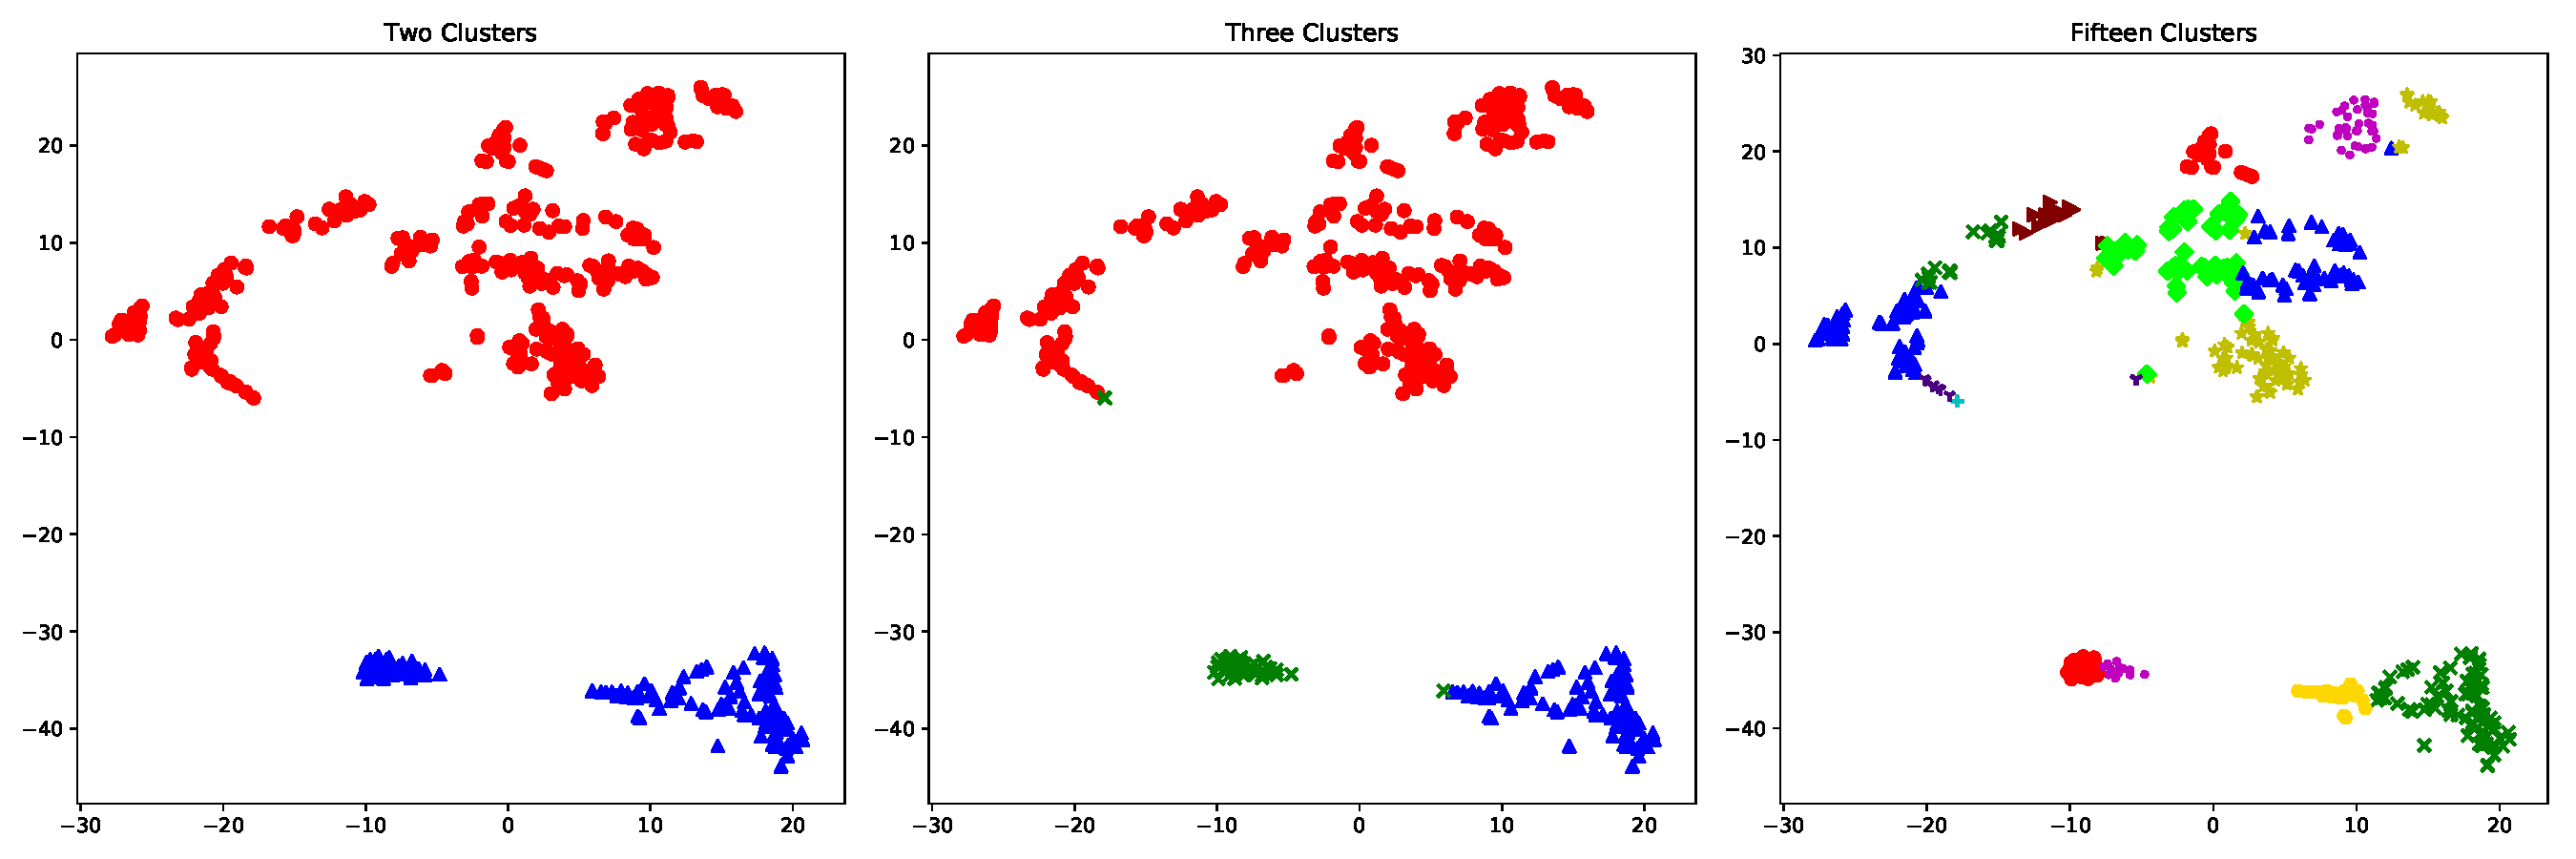
\includegraphics[width=1.0\textwidth]{images/kmeans_housing_tsne.pdf}
\end{center}
\label{fig:kmeans_housing_2d_comparison}
\end{figure}
\vspace{-0.5cm}

\subsubsection{Wine K-Means}
\textit{written by B.L.}\\

The wine dataset again presents a challenge due to its high feature count, the highest of all the datasets in this comparison as well as having one discrete feature. Dimensionality reduction helps to speed up calculation but does not show an improvement in evaluation index performance. The plot of evaluation indices in figure \ref{fig:kmeans_wine_indices_comparison} gives an indication for 2 (\gls{SI}, \gls{DB}), 3 (\gls{CH}), or 6 (\gls{CH}, \gls{DB}) clusters

\vspace{-0.5cm}
\begin{figure}[h]
\caption{K-Means Wine Dataset Indices by Number of Clusters}
\begin{center}
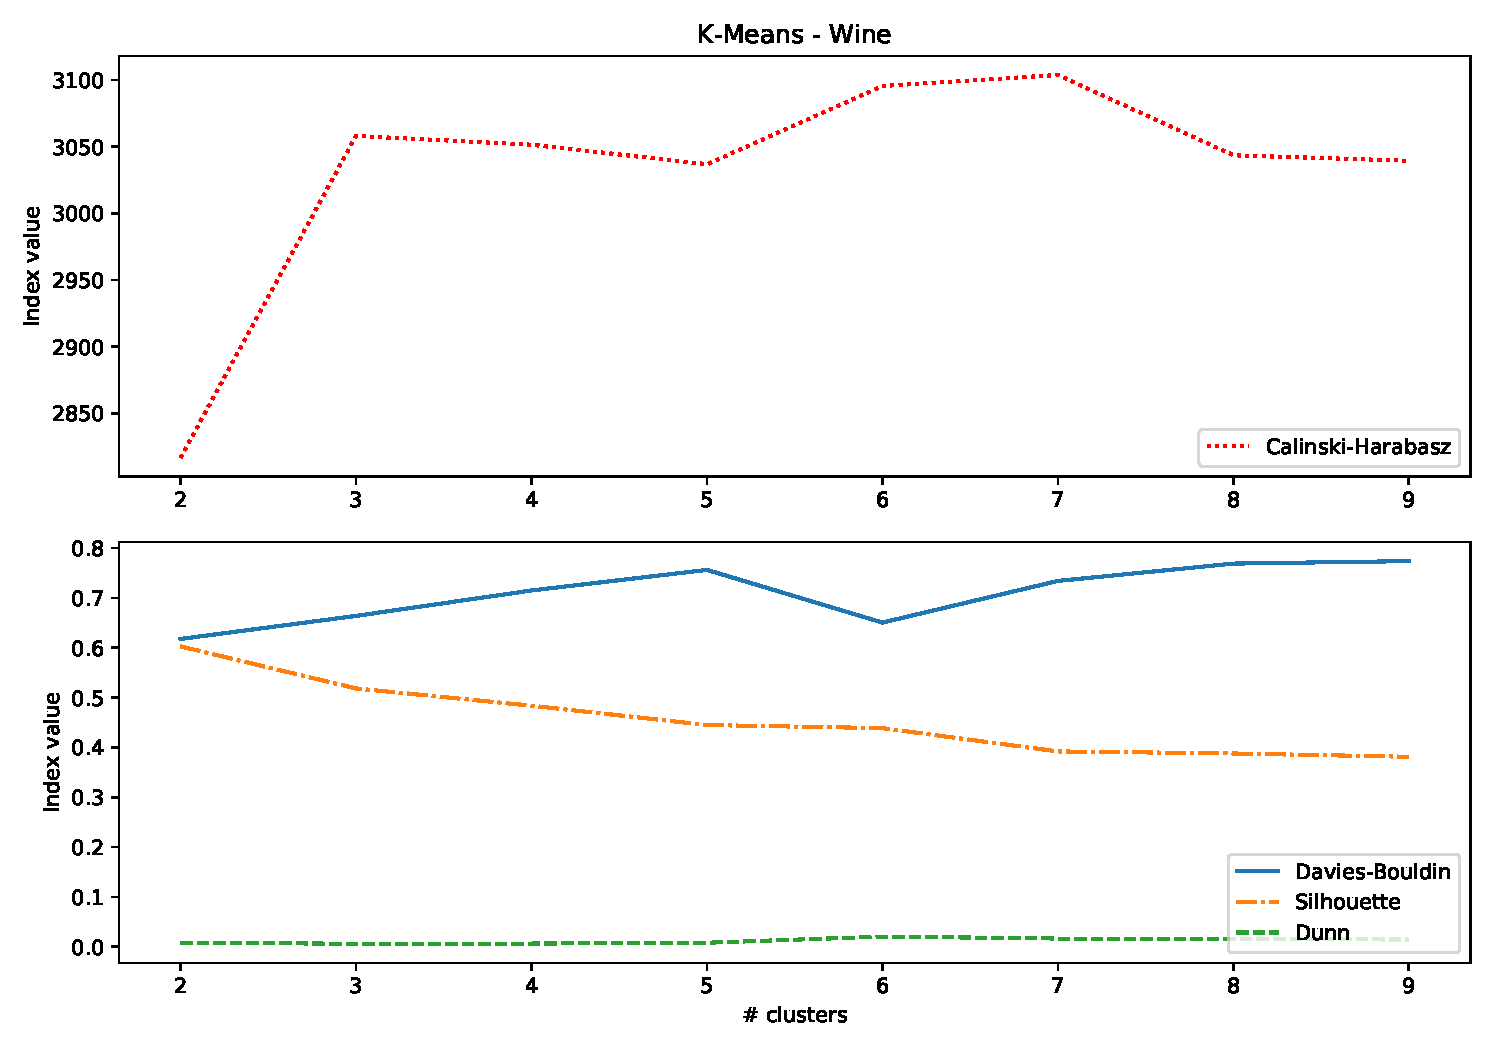
\includegraphics[width=1.0\textwidth]{images/kmeans_wine_index_plot.pdf}
\end{center}
\label{fig:kmeans_wine_indices_comparison}
\end{figure}

but looking at the two dimensional transformed data in figure \ref{fig:kmeans_wine_tsne} does not allow for any visual evaluation concerning the quality of fit.

%The result is inconclusive and without a focus on feature engineering other methods may be better suited to deal with this dataset.


\begin{figure}[H]
\caption{K-Means Wine Dataset Indices by Number of Clusters}
\begin{center}
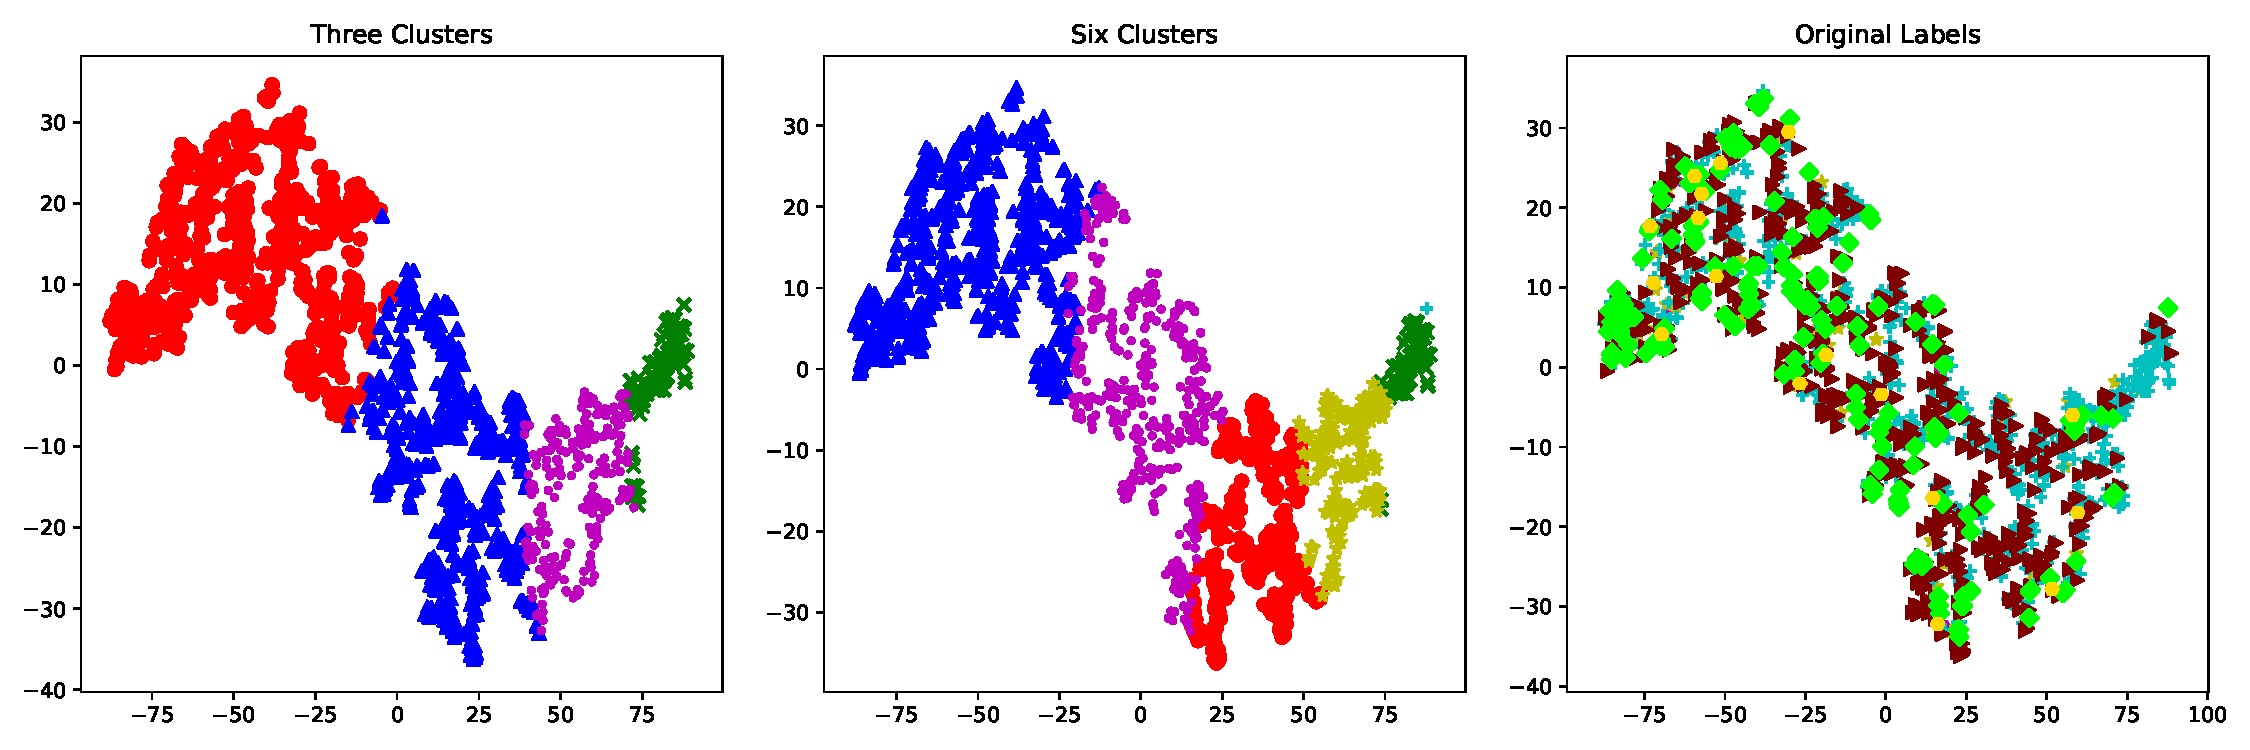
\includegraphics[width=1.0\textwidth]{images/kmeans_wine_tsne.pdf}
\end{center}
\label{fig:kmeans_wine_tsne}
\end{figure}

Looking back at the PCA step mentioned before, the picture becomes clearer when utilizing it as a visualization support and looking at a three dimensional representation of the transformed data in figure \ref{fig:kmeans_wine_3d_multi} gives a clearer understanding of how the clustering has worked out. The component driving the differentiation between clusters called \textit{PCA 1} captures 94\% of the variance and loadings show it being driven in large part by the two \textit{sulfur} concentration features.

\vspace{-0.5cm}
\begin{figure}[H]
\caption{Wine Dataset 3D Plot Clustering Options}
\centering
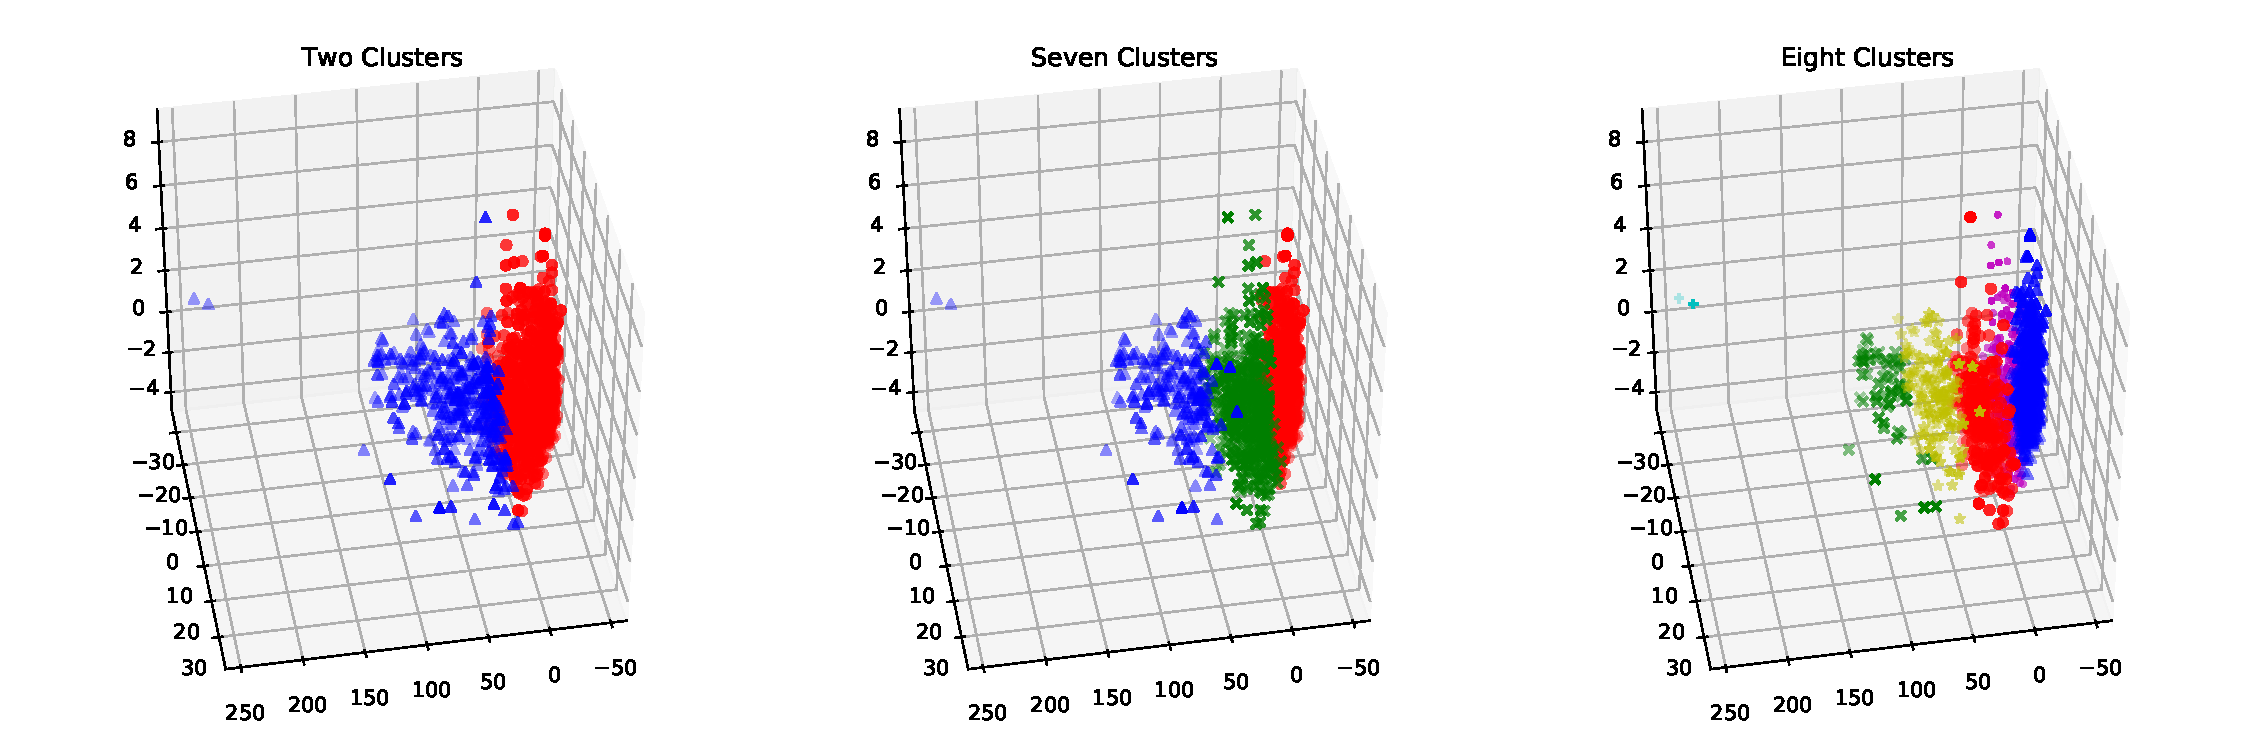
\includegraphics[width=1.0\textwidth]{images/kmeans_wine_3d_multi.pdf}
\label{fig:kmeans_wine_3d_multi}
\end{figure}

\vspace{-0.5cm}
\begin{wrapfigure}{r}{0.5\textwidth}
  \centering
    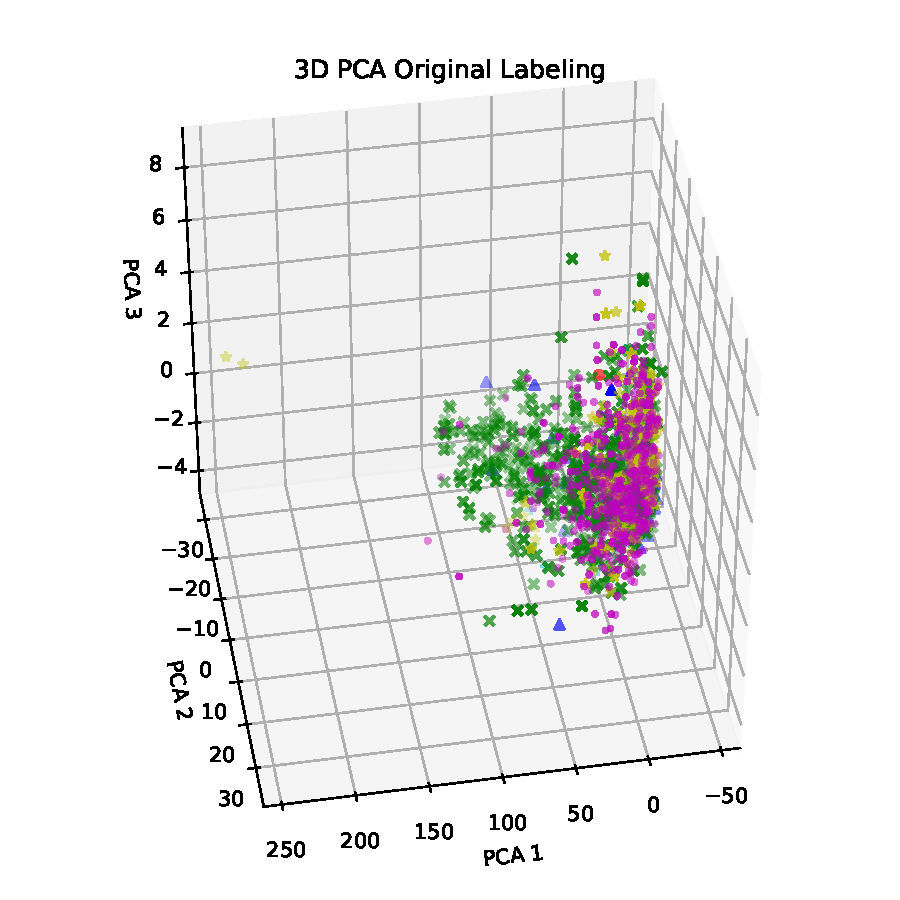
\includegraphics[trim={1cm 0cm 1cm 1cm},width=0.45\textwidth, clip]{images/kmeans_wine_pca_original.pdf}
  \label{fig:kmeans_wine_pca_original}
  \caption{Wine 3D Original Labeling}
\end{wrapfigure}
Looking at the original labeling of the data however shows the limitations of clustering and especially K-Means clustering for this data set. Figure \ref{fig:kmeans_wine_pca_original} shows the same projection as figure \ref{fig:kmeans_wine_3d_multi} but this time with the original labeling. The math on accuracy and recall at 19.8\% and precision somewhat better at 58.2\% also shows the less than optimal performance. However this is not unexpected when considering the strengths and weaknesses of K-Means described in section \ref{subsec:method_kmeans}: contiguous, non-overlapping, convex clusters can be captured well while at least this representation of the data displays a lack of these characteristics in the data set.

% \begin{itemize}
% \item What are the results and how are they measured?
% \end{itemize}

\section{Web Frontend and User Manual}
\label{sec:frontend_description}
\textit{written by L.B. and B.L.}\\

The frontend has been developed in Streamlit \cite{streamlit2018} in its latest version as of \today, 0.82.0 and can be accessed at \url{https://clustering.goethe.tech)}.
On the left there is a sidebar containing two collapsible content groups. One of them is called \mintinline[bgcolor=code-bg]{python}{Regular} and comprises controls for a single clustering method, the other named \mintinline[bgcolor=code-bg]{python}{Comparison} contains controls for a workflow that lets the user compare the different methods.
First off there is the \mintinline[bgcolor=code-bg]{python}{Regular} group. It provides a menu containing two dropdown lists. While the upper dropdown list can be used to select the dataset to be clustered, the second dropdown contains four different clustering algorithms to be applied: K-Means, Mean Shift, Spectral Clustering and Affinity Propagation. According to the selected clustering algorithm, the required input parameter can be set by dragging the slider on the respective widget. For this purpose, a message displays which kind of input parameter is required for the selected algorithm. 
Default values for different parameters vary with regard to the chosen dataset. We therefore provide slider widgets with different value ranges and varying default values according to the dataset to be clustered.
Once dataset and clustering technique are chosen, the \mintinline[bgcolor=code-bg]{python}{Calculate} button can be clicked to run the clustering procedure.
%For convenience, selected dataset and algorithms are listed above the result part once again. 
After the dataset is clustered, a two-dimensional projection plot of all data points is displayed in the main panel, distinguishing between different clusters with the help of distinct symbols and colors.

\begin{figure}[H]
%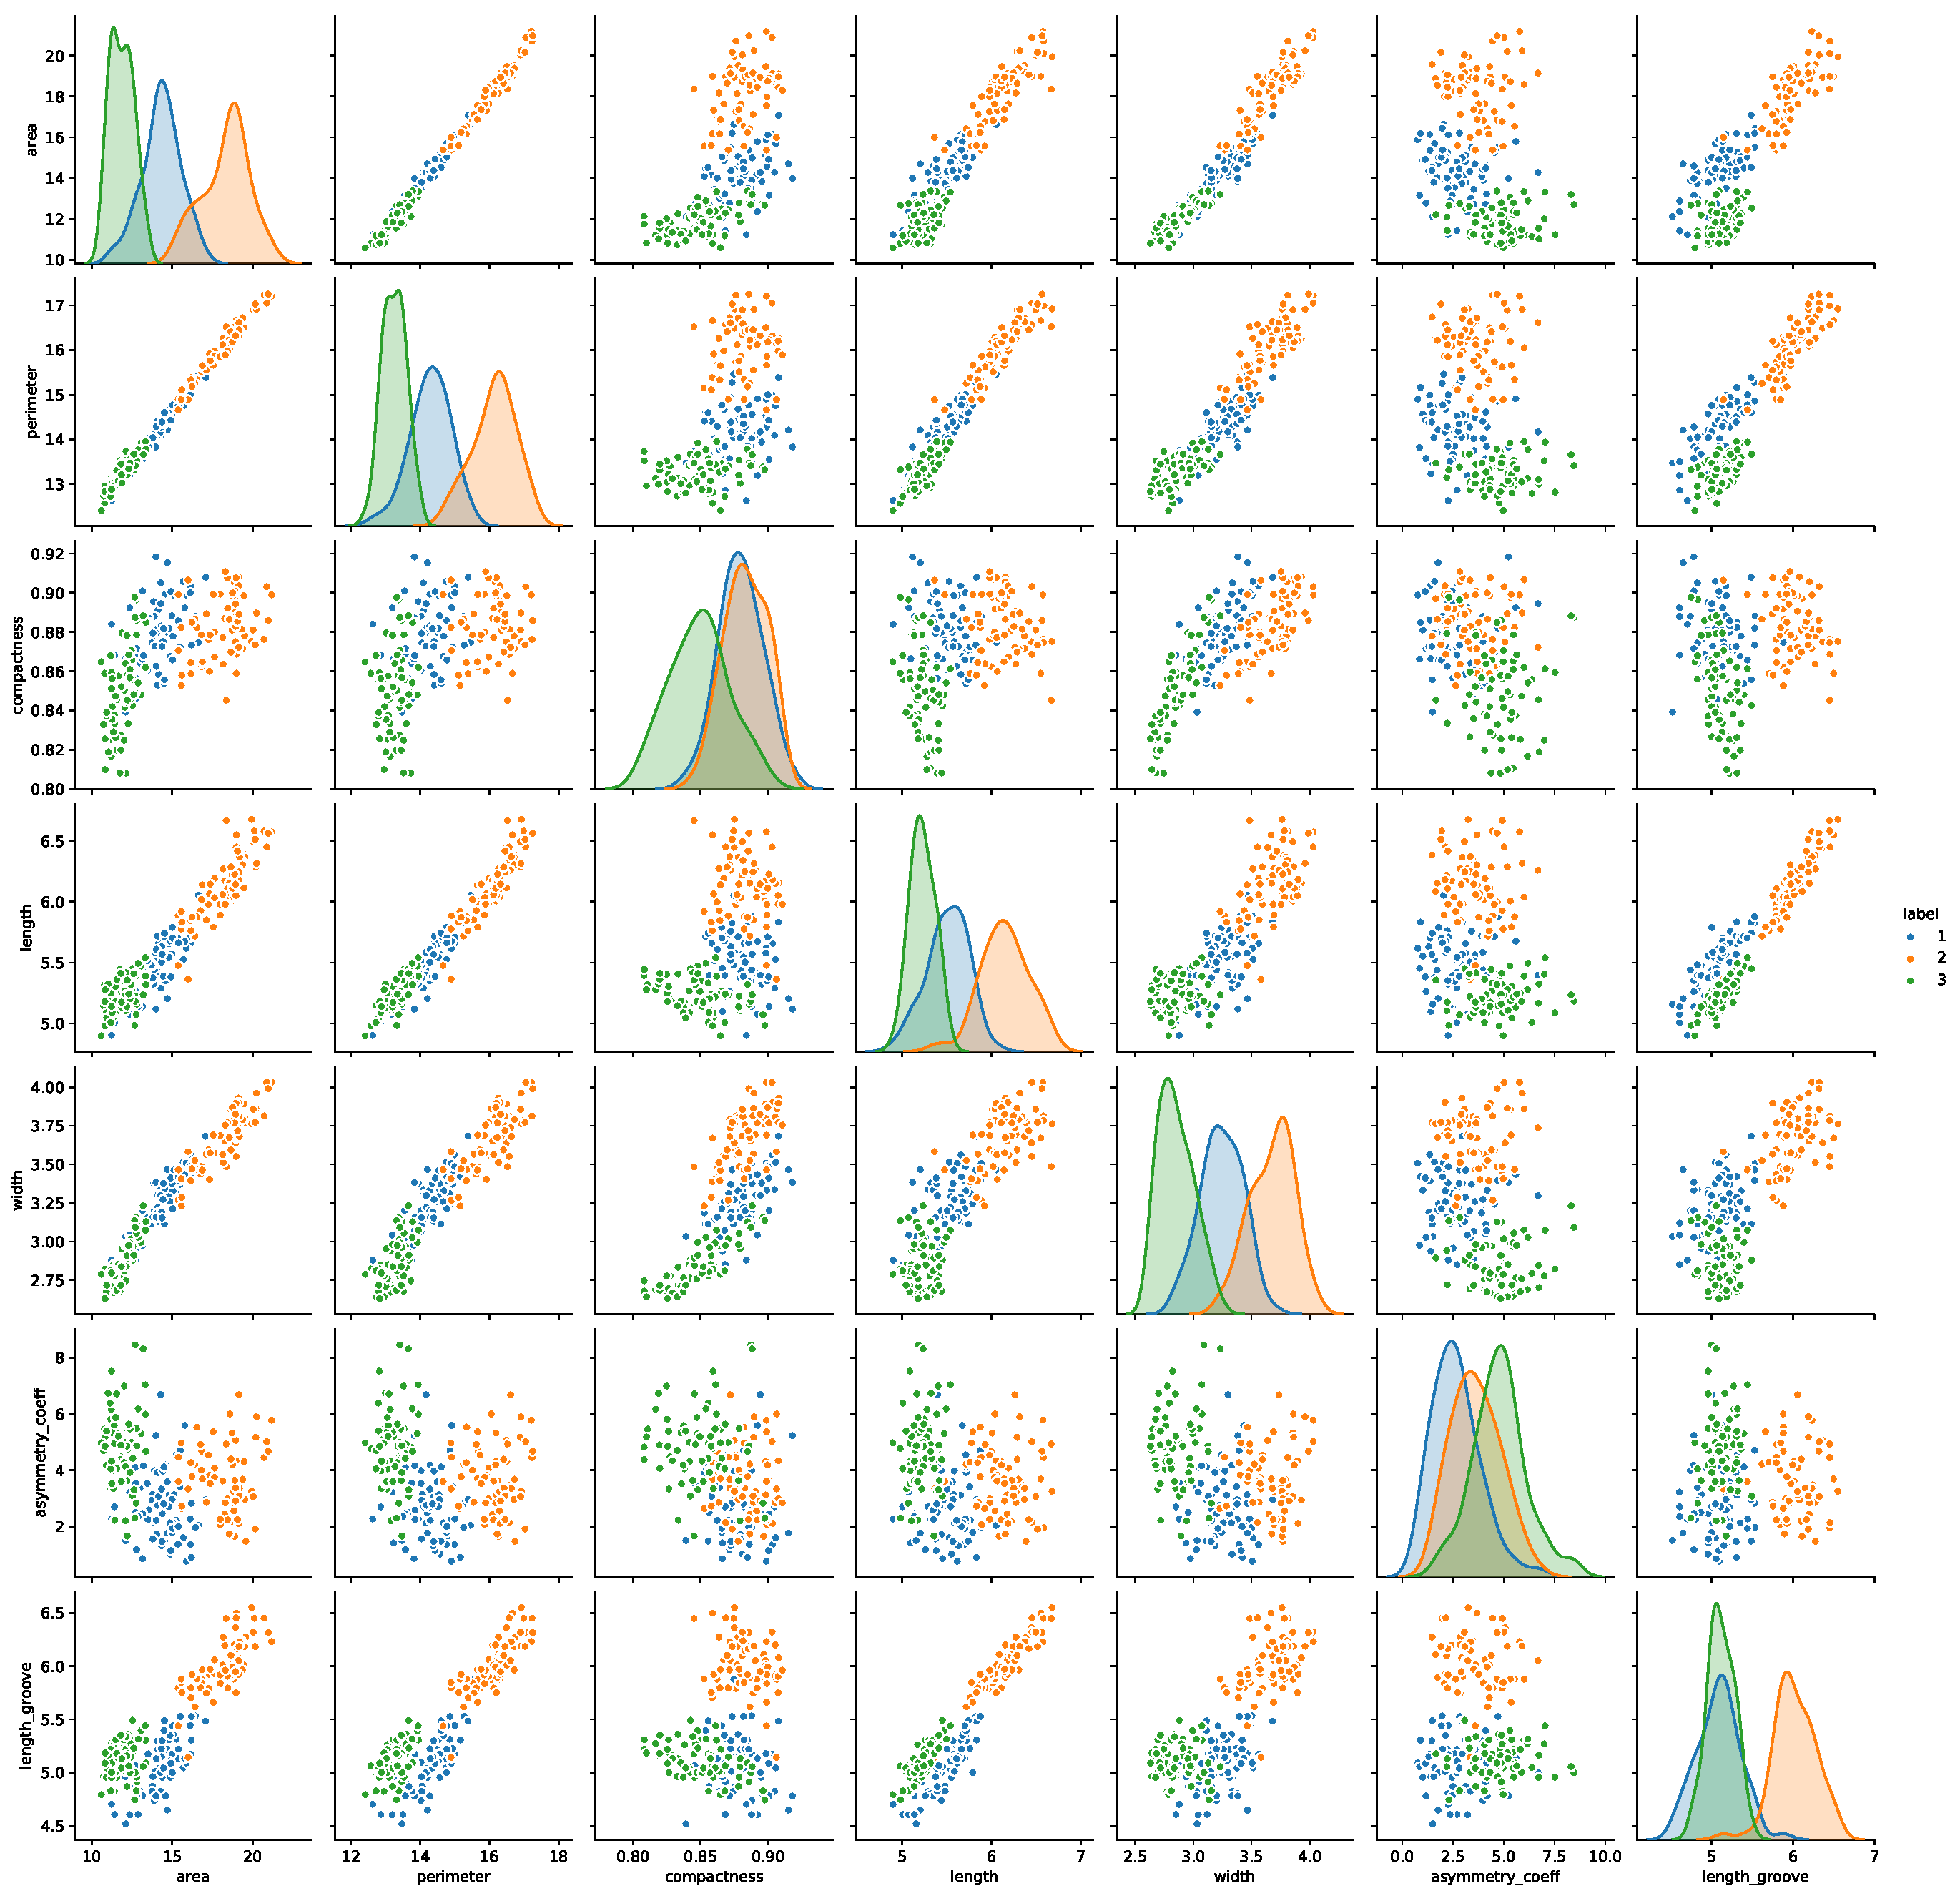
\includepdf[pages=-,scale=.4]{images/seeds_pairplot.pdf}
\begin{center}
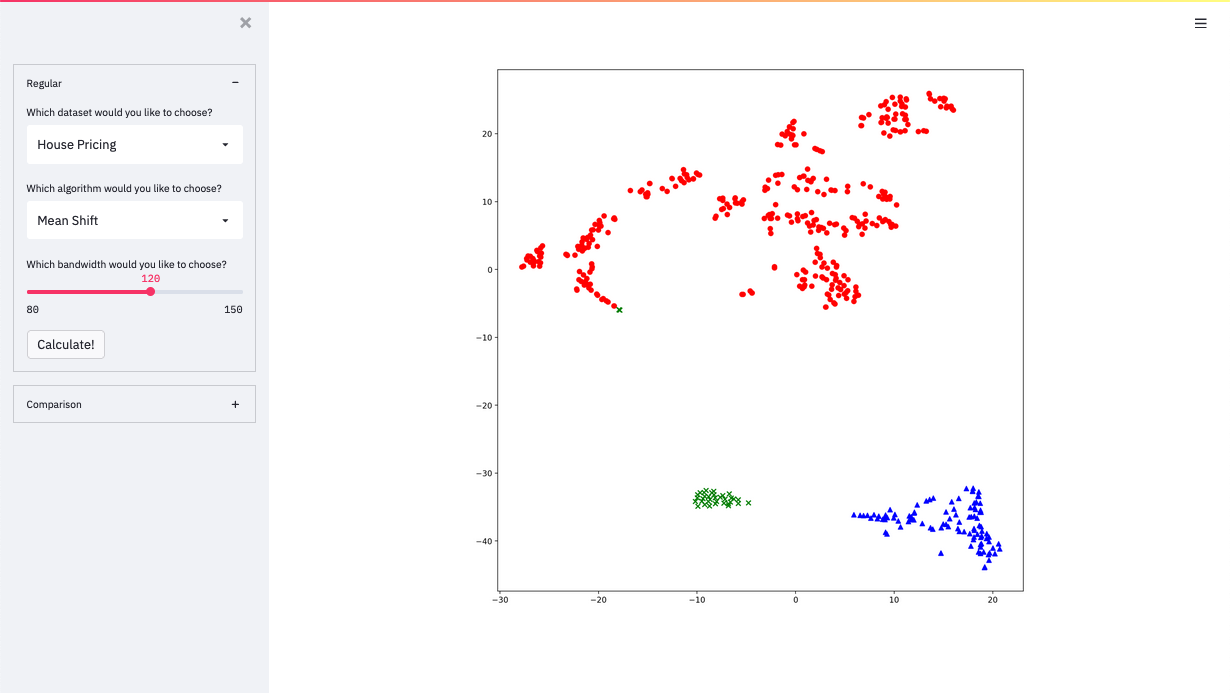
\includegraphics[width=0.9\textwidth]{images/frontend_regular.png}
\caption{Frontend Regular Mean Shift House Pricing Example}
\end{center}
\label{img:frontend_screenshot_regular}
\end{figure}

%In addition to that, we provide an evaluation module which can be used to compare different clustering strategies to each other. 
The \mintinline[bgcolor=code-bg]{python}{Comparison} group contains a singular drop down list which can be used to select the data set of interest. Below this menu there are the same type of sliders with the same functionality as described above, but in this case for all the methods at the same time. Clicking the \mintinline[bgcolor=code-bg]{python}{Compare} button runs all clustering methods with the specified parameters and displays them next to one another in the main panel, similar to the method described above. Located below these plots is a table containing the index values for each index described in section \ref{sec:evaluation_description} (rows) for each clustering method (columns).

\begin{figure}[H]
%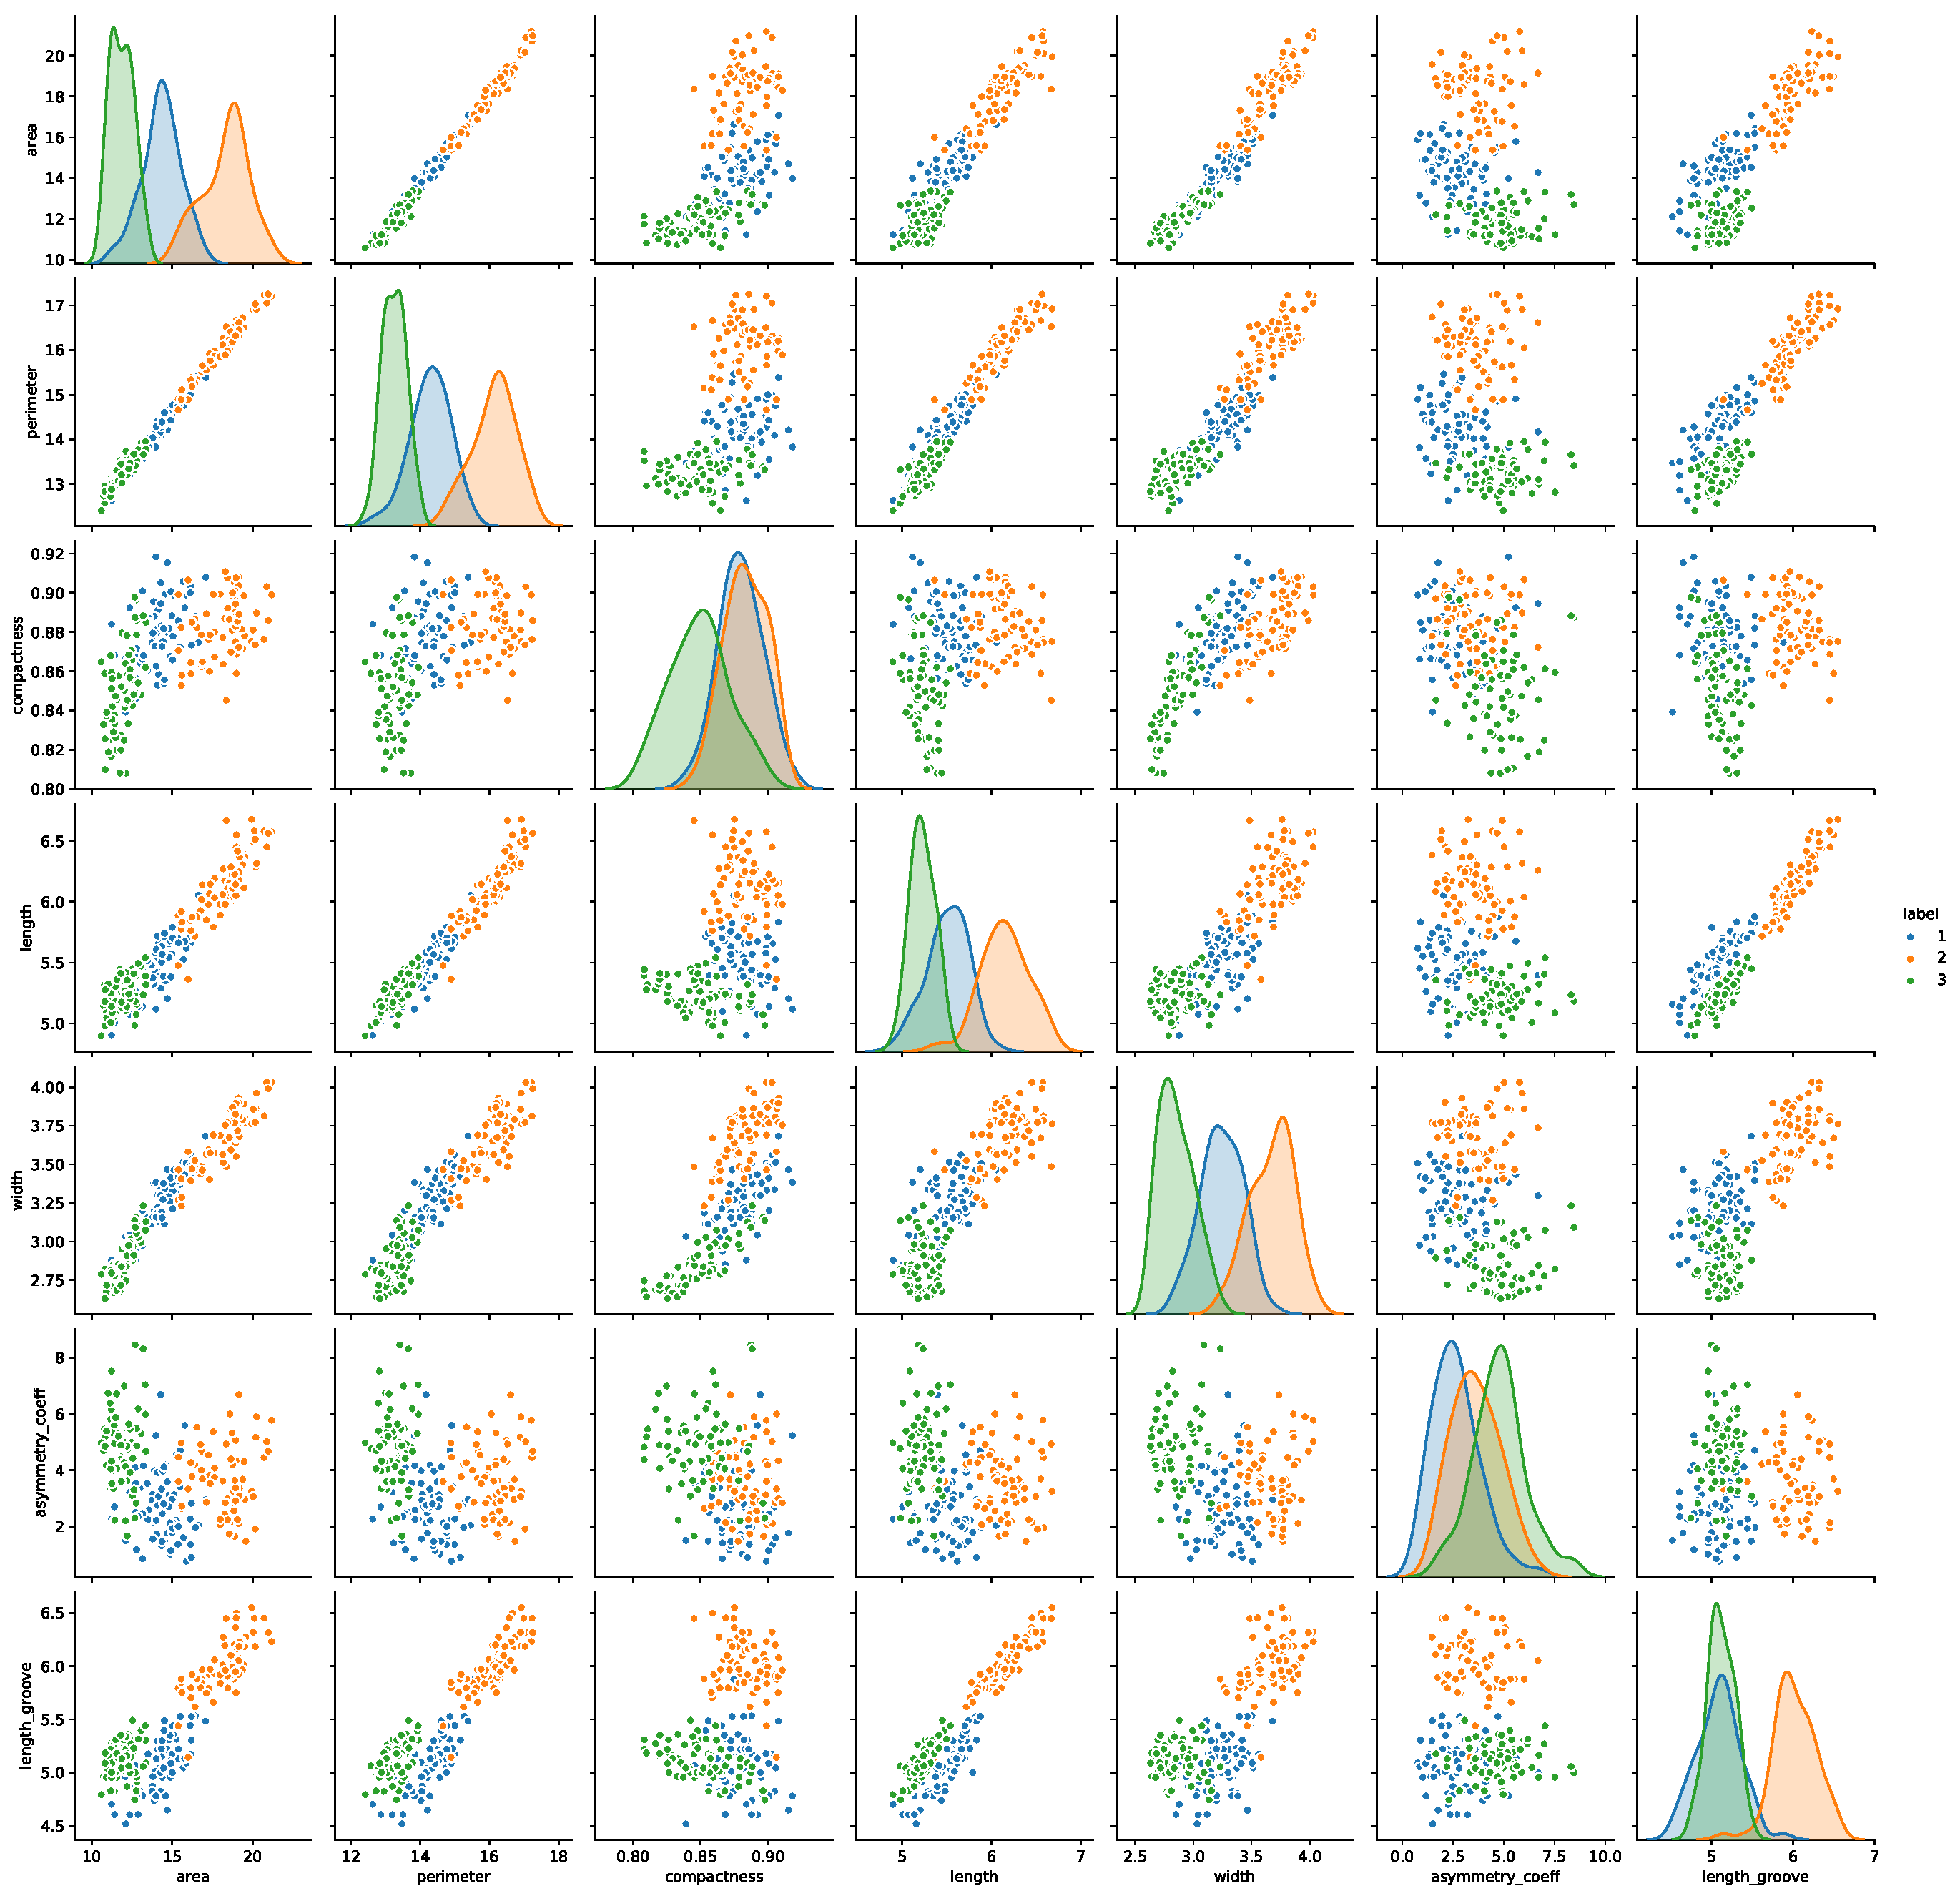
\includepdf[pages=-,scale=.4]{images/seeds_pairplot.pdf}
\begin{center}
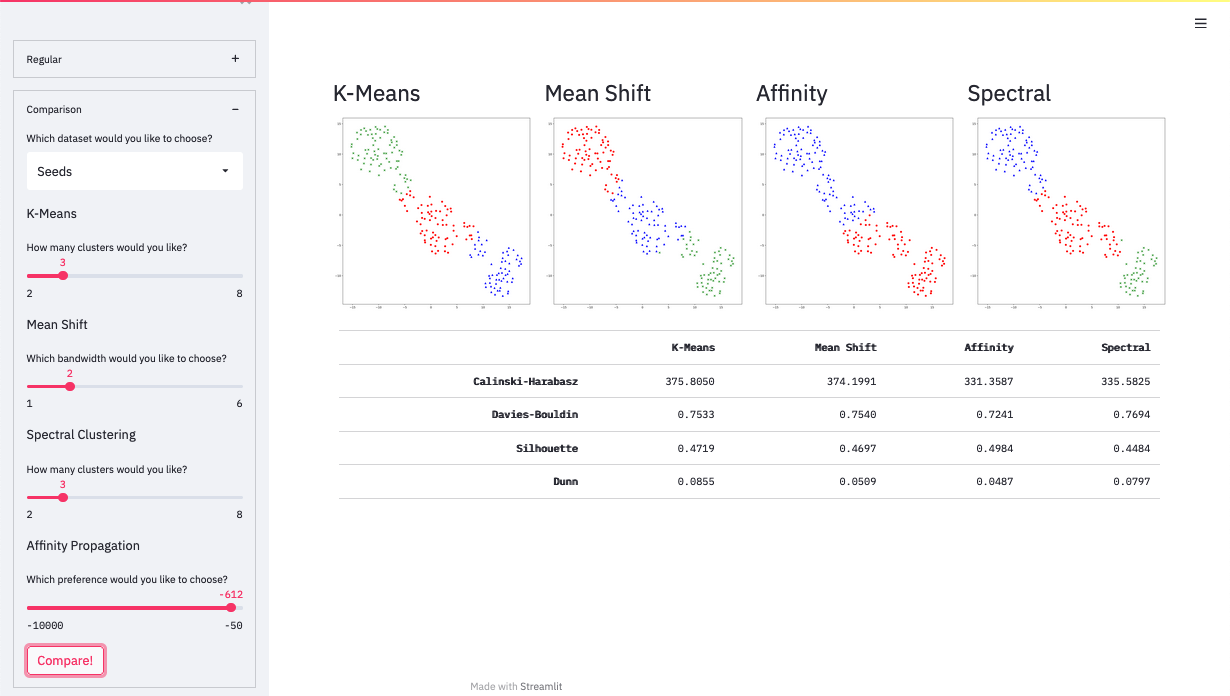
\includegraphics[width=0.9\textwidth]{images/frontend_comparison.png}
\caption{Frontend Comparison Seeds Example}
\end{center}
\label{img:frontend_screenshot_comparison}
\end{figure}

Our code implementation is divided into segments to isolate clustering procedures from projecting the data into 2D and from visualizing the results.

Each of the clustering techniques that can be selected for grouping data points is implemented in a separate file which is named according to the technique. To run one of the clustering algorithms, the dataset has to be handed over in form of an $n \times m$ matrix () consisting of n data points with m features. Moreover, a value for the algorithm specific parameter has to be provided. The \mintinline[bgcolor=code-bg]{python}{returns} parameter can be used to define what output format is expected. We provide the possibility to distinguish between returning the fitted estimator, an $n \times (m+1)$ - matrix consisting of $n$ data points with m features and a column containing a label for each data point (a task facilitated by \mintinline[bgcolor=code-bg]{python}{numpy} \cite{harris2020array}) or an $n \times 1$ vector, which only includes a label for each data point. These options exist in order to make it possible to return the right format for the task at hand, be it calculations for this work, for evaluation or plotting or inside the frontend itself. Running the clustering in its default mode, each technique returns the $n \times 1$ label vector.
For the K-Means algorithm, the additional parameter \mintinline[bgcolor=code-bg]{python}{state} can be set. This value is used to initialize the random number generator such that always the same results are yielded \cite{sklearn_api}.

In the top level \mintinline[bgcolor=code-bg]{python}{app.py} file, we implement all the functionalities concerning the frontend elements as well as choice of dataset and clustering technique. After reading the four different datasets using the \mintinline[bgcolor=code-bg]{python}{read_csv} method provided by pandas \cite{reback2020pandas, mckinney-proc-scipy-2010} non-numeric values in the data are converted to numeric and we calculate a version of the datasets transformed into 2D and cache it to speed up all following interactions because this step can take long for large data sets. The \mintinline[bgcolor=code-bg]{python}{tsne_transform} function performing this step also takes a state to ensure the resulting plots later will always look the same to ease comparability. To transform the datasets into 2D, inside \mintinline[bgcolor=code-bg]{python}{tsne_transform} we make use of the \gls{t-SNE} method provided by \gls{sklearn} \cite{sklearn_api}.

\mintinline[bgcolor=code-bg]{python}{t-SNE} is a method that facilitates displaying high-dimensional data in a 2D or 3D plot while nevertheless preserving local and global structures. This is done converting Euclidean distances between all data points in high dimensions into conditional probabilities such that high probabilities are allocated to similar data points while dissimilar data points are assigned a low probability. Afterwards, the same is done for all the data points projected into lower dimensions. The optimal projection of high-dimensional data points is finally found by minimizing the mismatch between calculated probabilities between points in high and in low dimensions \cite{van2008visualizing}.

As described earlier, we not only provide dropdown lists to enable the choice of a dataset as well as a clustering technique, but also adapt the slider widget label according to the required input parameter for the chosen algorithm. We define parameter value ranges along with default values appropriate to the chosen dataset. 
To run the clustering procedure, an event handler listens for click events on the \mintinline[bgcolor=code-bg]{python}{Calculate} button. According to the selected clustering algorithm, we call the respective clustering function and hand over the dataset as an $n \times m$ - matrix as well as the technique specific parameter value which was selected with the help of the slider widget.

Largely the same happens when using the \mintinline[bgcolor=code-bg]{python}{Comparison} workflow. The main difference is in the fact that selecting an algorithm is not required because all of them will be run one after the other and plotted next to each other accordingly. The comparison table is then calculated by using the \mintinline[bgcolor=code-bg]{python}{evaluation} module, returning index values and transforming them into an overview.

The plotting as described above is based on \gls{t-SNE} transformation and executed by calling the \mintinline[bgcolor=code-bg]{python}{plot_tsne_2} from the plotting module. The resulting figure comprises scatter plots from the Matplotlib visualization function \mintinline[bgcolor=code-bg]{python}{pyplot} \cite{Hunter:2007} overlayed atop each other for each cluster. This results in one single plot containing all data but each cluster differentiated by color and marker shape making it easy to distinguish between clusters.

\section{Conclusion}
%\begin{itemize}
%\item Summarize the main points and achievements
%\item Add your own assessment/criticism on the topic
%\end{itemize}

After brief conclusions on each clustering method, a more general conclusion follows, discussing observations and particularities that stand out when looking at the functioning and results for all methods on all data sets with all evaluation methods.

\textit{K-Means} - Generally K-Means clustering is a fast, easy to use and reliable method to cluster data. For house pricing, seeds and mall customer data it works well at segmenting into separate partitions which can be inspected visually to be what a human would describe as distinct clusters. When the underlying structure of the data lends itself to the globular type of cluster shapes K-Means is known for, like the seeds data set, the result is dependable as the use of classification scores has shown. House pricing and wine quality data show that high dimensional and overlapping data poses a challenge because especially in the wine data set (barely any separation) K-Means \textit{will} find clusters of similar size and shape even if those do not represent the underlying data well.

\textit{Mean Shift} - Normally, Mean Shift algorithm is known to work best on low-dimensional data sets but nevertheless, it performed better on our high-dimensional data sets about Boston House Pricing and Red Wine Quality in contrast to the low-dimensional data sets about Seeds and Mall Customer Data. As Mean Shift is density-based, this phenomenon can be explained taking not only data set dimensionality but also density into account. For the best Mean Shift performance, data sets consisting of dense regions which are distant from each other are required.
One main advantage is that Mean Shift neither makes any assumptions about the number of resulting clusters, nor on their shape. The only parameter that is required is the kernel's radius which may often be easier to estimate for real world data than the number of natural groups.
The optimal value for the bandwidth parameter has to be evaluated for each data set individually.

\textit{Affinity Propagation} - Overall, we would rate Affinity Propagation as a medium cluster algorithm because it can compute a good clustering, but this depends on the given data set and on the parameter values. Affinity Propagation clustering results for the first and second data set seem to be suitable, but those for the third and fourth data set do not represent plausible structures. Applying the Affinity Propagation algorithm without fitting the parameters will not result in a good clustering. This happened in all four data sets. Sometimes, the algorithm does not converge which makes it rather unstable. An advantage of Affinity Propagation is that it does not require the number of clusters beforehand. Because of this property, Affinity Propagation is good if you don’t know much about the data set, but the calculation is slowly because it depends on the data points in the data set. It also works better with data sets consisting of low dimensions like the Mall Customers and the Seeds data set. For a data set which has many dimensions, Affinity Propagation will find a lot of clusters.

\textit{Spectral Clustering} – To sum up, the Spectral Clustering algorithm is a very popular and easy implementable algorithm. It is computationally expensive for large data sets such as the Wine Quality data set. The reason for that is that eigenvalues and eigenvectors need to be computed and then clustering is being done on these vectors. For large data sets this may increase
time complexity. \newline
In general, Spectral Clustering is not making any problems with the data sets we have chosen. The main advantage of Spectral Clustering is that it is applicable for non-convex geometries and there is no assumption made about the shape or form of the clusters even intertwined spirals are possible. Only waiting for the plot to be build can put you on hold.\\

As a high level overview it can be said that no one single algorithm outperforms the others in all or most circumstances. Each has particular advantages which could be seen for the different data sets. Some particularities can however be noted. Using K-Means and Mean Shift can regularly produce remarkably similar clustering results for the data sets at hand despite their different methods of arriving there. 

For visually reasonable clusterings, \gls{CH} often sees highest values for K-Means clustering, which makes sense given its construction (see section \ref{sec:evaluation_description}). However, its meaningfulness does seem to break down when there is an excessive number of clusters, possibly skewing the perception of clustering success when solely relying on this type of evaluation as can be seen in table \ref{tab:evalutaion_table}. On this topic it should be reiterated that using evaluation indices on the same algorithm for different parameter configurations might be more meaningful than comparing different algorithms when not taking additional information into account. Also relying on a single measure can lead to one sided conclusions.

A few observations on the application of the clustering algorithm implementations: Affinity Clustering seems to be somewhat unstable when trying out different preference parameter values, regularly failing to converge even when significantly increasing the iteration limit. Run time for Affinity Clustering and Spectral Clustering can be notably longer than Mean Shift and especially the utilized fast method for K-Means.

Given the opportunity to compare clustering results with original labelling for two of the data sets confirms the expectation that accurately assigning observations to groups is harder when separation is lacking. This is particularly evident in the results for Wine Quality data where all algorithms do find clusters but the actual data is highly dispersed and overlapping.

All in all, it is highly dependent on the given data set in terms of its dimensionality and distribution of data points which algorithm should be applied to find a reasonable clustering result.

\newpage

%print glossary
\printglossary[style=altlist,title=Glossary]
 
%print abbreviations
\printglossary[type=\acronymtype,style=long]
 
%print symbols
\printglossary[type=symbolslist,style=long]

\newpage

\bibliography{bib}
\bibliographystyle{unsrt}

\end{document}
